\documentclass{uofsthesis-cs}

% Documentation for the uofsthesis-cs class is given in uofsthesis-cs.dvi
% 
% It is recommended that you read the CGSR thesis preparation
% guidelines before proceeding.
% They can be found at http://www.usask.ca/cgsr/thesis/index.htm

%%%%%%%%%%%%%%%%%%%%%%%%%%%%%%%%%%%%%%%%%%%%%%%%%%%%%%%%%%%%%%%%%%%%%%%%%%%%%%
% FRONTMATTER - In this section, specify information to be used to
% typeset the thesis frontmatter.
  \usepackage{graphicx} 
\usepackage{cite}   
\usepackage{url}  
\usepackage{todonotes}
\usepackage{textcomp}
%%%%%%%%%%%%%%%%%%%%%%%%%%%%%%%%%%%%%%%%%%%%%%%%%%%%%%%%%%%%%%%%%%%%%%%%%%%%

% THESIS TITLE
% Specify the title. Set the capitalization how you want it.
\title{SynVisio: A Multiscale Tool for Visualizing Genomic Conservation}

% AUTHOR'S NAME
% Your name goes here.
\author{Venkat Kiran Bandi}

% DEGREE SOUGHT.  
% Use \MSc or \PhD here
\degree{\MSc}         

% THESIS DEFENCE DATE
% Should be month/year, e.g. July 2004
\defencedate{December/2019}


% NAME OF ACADEMIC UNIT
%
% The following two commands allow you to specify the academic unit you belong to.
% This will appear on the title page as
% ``<academic unit> of <department>''.
% So if you are in the division of biomedical engineering you would need to do:
% \department{Biomedical Engineering}
% \academicunit{Division}
%
% The default is ``Department of Computer Science'' if these commands
% are not given.
%
% If you are in a discipline other than Computer Science, uncomment the following line and
% specify your discipline/department.  Default is 'Computer Science'.
% \department{If not Computer Science, put the name of your department here}

% If you are not in a department, but say, a division, uncomment the following line.
% \academicunit{Put the type of academic unit you belong to here, e.g. Division, College}


% PERMISSION TO USE ADDRESS
%
% If you are not in Comptuer Science you will want to change the
% address on the Permission to Use page.  This is done using the
% \ptuaddress{}.  Example:
%
% \ptuaddress{Head of the Department of Computer Science\\
% 176 Thorvaldson Building\\
% 110 Science Place\\
% University of Saskatchewan\\
% Saskatoon, Saskatchewan\\
% Canada\\
% S7N 5C9
% }

% ABSTRACT
\abstract{
Due to rapid advancements in sequencing technologies high resolution genomic data is readily available for a wide range of species. However, analysing this huge volume of data is still a tedious task. While most genomic analysis tasks can be automated some still require human judgement and manual interpretation. One example of such a task is synteny analysis. Synteny is a key tool in comparative genomic research - it is the study of homologous regions within chromosomes of the same or different species. Visualizing synteny can help researchers in understanding the \textbf{location, size and orientation} of shared sequences among genomes of interest. However, the current tools which exist for synteny analysis are stand-alone programs or command line tools that are difficult to use and that offer very little interactivity. In this paper we provide a decentralized web-based environment for browsing syntenic blocks with multiple visual representations in the form of linear charts, hive charts and dot plots. Our tool also makes it easy to save and revisit graphs so that researchers can iteratively refine their plots and compare them with previous revisions for changes. We present SynVisio, a multiscale synteny analysis tool that provides multiple visualizations of genome collinearity for easy exploration across different scales from the whole genome level all the way down to the individual gene block level.
}

% THESIS ACKNOWLEDGEMENTS -- This can be free-form.
\acknowledgements{
Acknowledgements go here.  Typically you would at least thank your supervisor.
}

% THESIS DEDICATION -- Also free-form.  If you don't want a dedication, comment out the following
% line.
% \dedication{This is the thesis dedication (optional)}

% LIST OF ABBREVIATIONS - Sample  
% If you don't want a list of abbreviations, comment the following 4 lines.
\loa{
\abbrev{DNA}{Deoxyribonucleic Acid}
\abbrev{FASTA}{Fast All}
\abbrev{SVG}{Simple Vector Graphics}
}

%%%%%%%%%%%%%%%%%%%%%%%%%%%%%%%%%%%%%%%%%%%%%%%%%%%%%%%%%%%%%%%%
% END OF FRONTMATTER SECTION
%%%%%%%%%%%%%%%%%%%%%%%%%%%%%%%%%%%%%%%%%%%%%%%%%%%%%%%%%%%%%%%%

\begin{document}

% Typeset the title page
\maketitle

% Typeset the frontmatter.  
\frontmatter

%%%%%%%%%%%%%%%%%%%%%%%%%%%%%%%%%%%%%%%%%%%%%%%%%%%%%%%%%%%%%%%%
% FIRST CHAPTER OF THESIS BEGINS HERE
%%%%%%%%%%%%%%%%%%%%%%%%%%%%%%%%%%%%%%%%%%%%%%%%%%%%%%%%%%%%%%%%
\chapter{Introduction}

With the emergence of new sequencing systems genomic data is being generated at an unprecedented rate.Almost two decades back \textbf{The Human Genome Project} took 13 years and over 3 billion dollars to sequence the entire human genome whereas the same information can be sequenced today in under an hour for 1000 dollars.This rapid improvement in sequencing has improved the availability of high resolution genomics data and has helped researchers in tackling a wide range of biological questions.


% reference to https://www.genome.gov/human-genome-project/Completion-FAQ


An important field in biological research where genomic data is extensively used is comparative genomics.It involves comparing genomic information between different species to understand their similarity.A genome of an organism consists of its complete set of DNA as a collection of genes where every gene is a sequence that is responsible for one or more traits in that organism.Comparing genomic sequences between two different organisms can help researchers in understating their evolutionary relationship as similar sequences can often mean that the genes have the same function.Such similar sequences are referred to as homologous sequences and they indicate shared ancestry.As organism evolve overtime and diversify into different species they retain parts of their DNA from their common ancestor.The study of these conserved homologous regions is called \textbf{Synteny}. 

While a huge part of comparing large scale genomic sequences is purely computational and thus can be automated human judgement is still vital in syteny analysis.Visual data exploration for example can help researchers in easily identifying similarities among large scale genomes as humans are intuitively good at picking out patterns in pictures and visuals.Synteny visualization commonly involves visualizing genomes at the whole genome level or the individual chromosome level and representing similar genes either by connected links or similar colored regions.Syntenic data analysis can often be an iterative process where researchers visualize computational results multiple times under various parameters such as the size and orientation of similar genes based on a given biological hypothesis.

The choice of visual encoding in the representation of syntenic relationship is dependant on the kind of analysis that is being done by the researchers.Certain graphical representations like dot plots where every conserved gene is represented as a point on a two dimensional matrix, are useful in analyzing extremely large genomes in a single representation as shown in Figure \ref{fig:ch_1_dot_plot} while other representations like linear horizontal plots where syntenic links are represented as coloured ribbons connecting similar regions are useful in performing a more in depth analysis as the conserved regions are more visually prominent.Additionally Circos plots which use a circular ideogram layout as shown in Figure \ref{fig:ch_1_circos_plot} are also frequently used by researchers in publications as they can be aesthetically pleasing to the general public while still being informative enough for researchers.

With such varied graphical representations, arriving at the right form of visualization can be difficult and any system that offers only a single kind of visual encoding can become limited in its usability for a wide range of biological scenarios.Apart from looking at synteny in multiple representations researchers are also often interested in  investigate specific conserved regions further and thus require the visualization system to be adaptive based on the genomic scale of interest.Thus visualizations systems need to go beyond acting as basic chart generating systems and instead offer a rich interactive experience where researchers can explore sequences from the whole genome level all the way down to the individual gene level in multiple graphical representations.

A key part of every visualization system is the data that drives it and genomic data owing to its large volume, is being increasingly managed and distribution through several online databases like NCBI and genBank.This rapid dissemination of data across the internet has also created a need for visualization systems to be easily available across the web so researchers can collaborate and share their work.


\begin{figure}
\centering
\begin{minipage}{.5\textwidth}
  \centering
  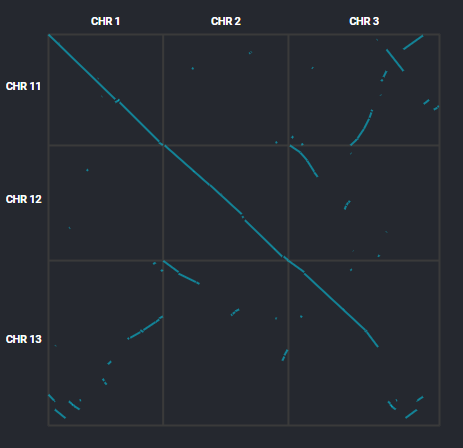
\includegraphics[width=.75\linewidth]{images/ch_1_dot_plot.PNG}
  \captionof{figure}{Dot plot}
  \label{fig:ch_1_dot_plot}
\end{minipage}%
\begin{minipage}{.5\textwidth}
  \centering
  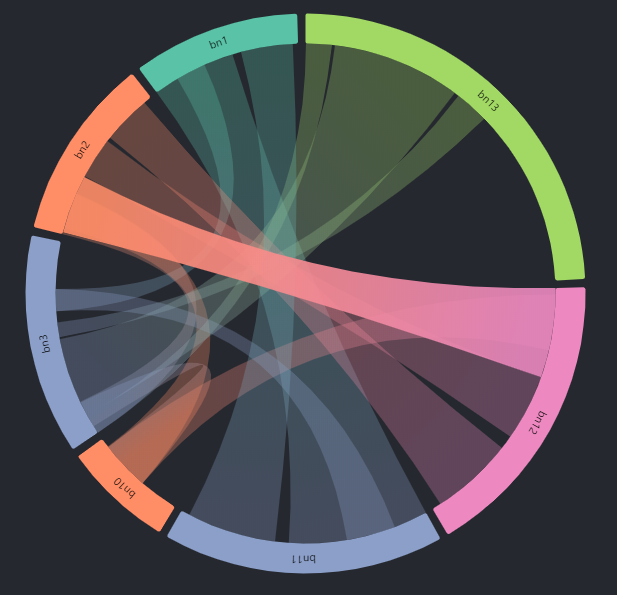
\includegraphics[width=.75\linewidth]{images/ch_1_circos_plot.PNG}
  \captionof{figure}{Circos Plot}
  \label{fig:ch_1_circos_plot}
\end{minipage}
\end{figure}


\section{Problem and Motivation}

The problem addressed in this thesis is: \textit{existing synteny tools are limited in their accessibility, offer little or no interactive experience and aren't integrated with the existing synteny detection tools to offer a seamless experience.}

Owing to the complexity involved in generating visualizations of large scale genomes, synteny visualization tools are largely command line based or stand alone programs limited to working in specific operating systems.This combined with the steep learning curve in using these systems means that a large set of these tools aren't accessible to the wider science community.Of the few online visualizations systems that exist, most act as simple chart generation systems instead of offering researchers chance to explore their datasets.This has largely pushed visualization into the report generation stage instead of the  iterative hypothesis testing phase of the research cycle.

Understanding genomic conservation is crucial for researchers as it has applications in a wide variety of scenarios such as predicting whole genome duplication events,sequencing extremely large genome sequences like wheat and classifying the proximity of different species in their evolutionary history.
While visualization systems are important as report generating tools that can create publication ready charts they need to move to earlier stages of the stages of the research cycle to accelerate the process of hypothesis testing.
Researchers should have the ability to interact with their datasets and change parameters in real time to see their results in easily understandable visual,
which in turn can let researchers explore a wide range of biological scenarios in a short span of time.
% refer vgsc

\section{Solution}

\begin{figure}
  \centering
  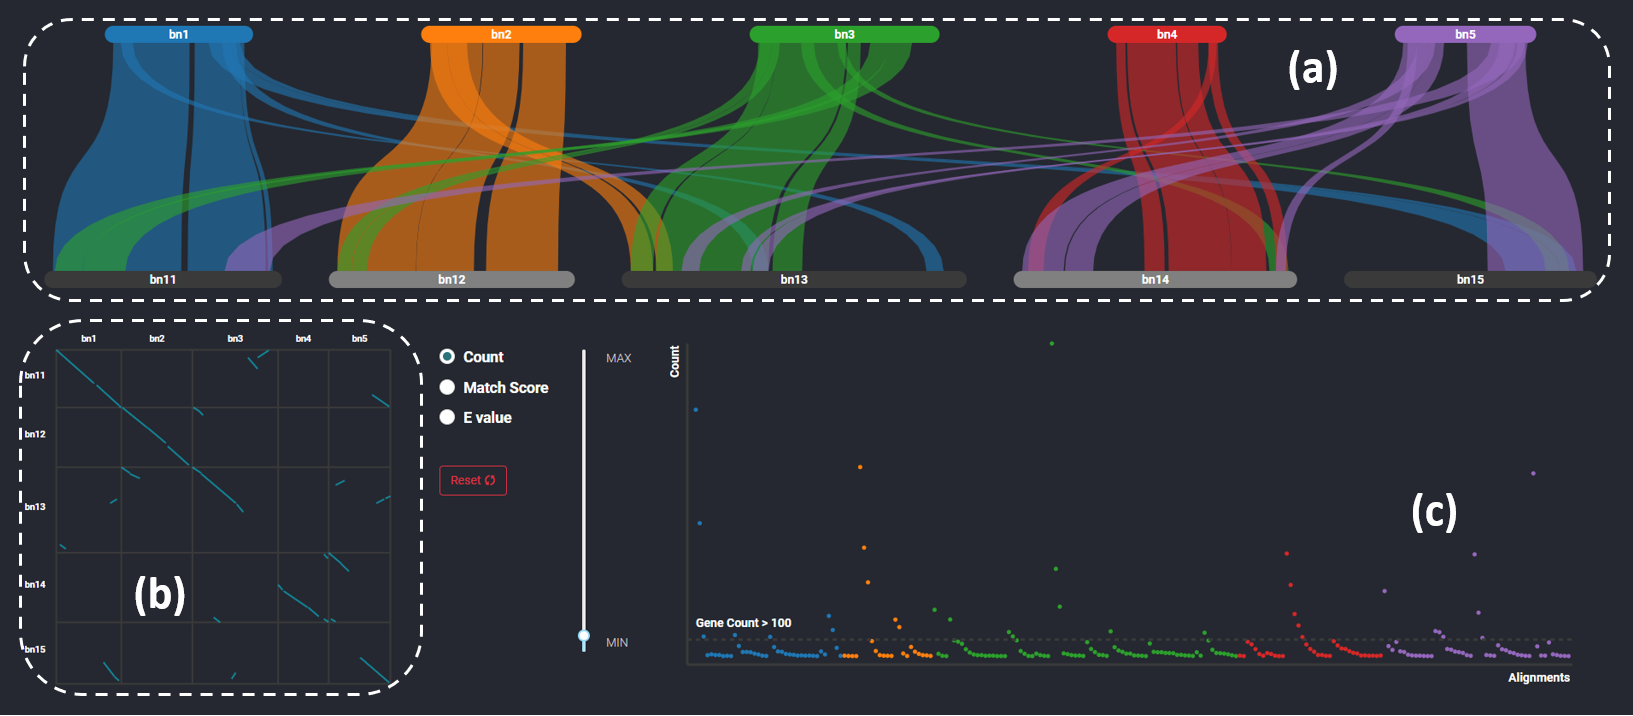
\includegraphics[width=.75\linewidth]{images/ch_1_dashboard.PNG}
  \captionof{figure}{Syteny Dashboard visualizing genome collinearity in Bn(Brassica Napus) with the following components: \textbf{a)} Linear Link Plot with connected ribbons representing collinear gene blocks. \textbf{b)}Dot plot where every collinear gene is represented by a point and contiguous collinear blocks are shown as lines. \textbf{c)} Filter panel representing all the collinear blocks based on the count of their genes with ability to refine results using slider to the left.  }
  \label{fig:ch_1_dashboard}
\end{figure}

To address the lack of proper analysis tools in syteny research we developed \textbf{SynVisio} a decentralized web based environment for browsing syntenic blocks with multiple visual representations across different scales from the whole genome level to the individual gene level.

\textbf{SynVisio} can directly work with results of existing syteny detecting tools like MCScanX and DAGChainer and can visualize conservation in multiple representations.It works in two modes,the basic synteny analysis mode lets users compare chromosomes in the same genome or between two genomes and the information is visualized as Horizontal linear plots,Dot plots or both as shown in Figure \ref{fig:ch_1_dashboard}.For visualizing synteny across several genomes simultaneously \textbf{SynVisio} offers a Multi-level analysis mode where synteny is visualized in stacked horizontal plots or Hive plots.\textbf{SynVisio} offers a rich interactive experience by letting users switch graphs in real time and explore data from genome level all the way down to the individual gene level.Users can do this by simply clicking on any two chromosomes when looking at a visualization in the genome level and then further step down from the individual chromosome level by clicking on a particular gene block to look at its constituent  genes and their orientation. Additionally users also have the ability to annotate their charts with additional genomic data in the form of tracks above the genomes or chromosomes which can be visualized as heat-maps,histograms or scatter-plots.



By default \textbf{SynVisio} lets users select the chromosomes that they wish to explore and then visualizes the conserved gene blocks in a dashboard that shows both the Horizontal linear plot and a Dot plot along with a filter panel where users can refine the results using a slider based on the level of similarity and the number of contiguous genes in a conserved block.
As users explore synteny using \textbf{SynVisio} it offers them the ability to records their interactions as snapshots which can be revisited or reset giving the ability to explore multiple scenarios and switch between them.The system also indexes all the conserved genes in the browser thus letting users quickly lookup genes by their gene IDs to see which conserved blocks they belong to.Finally \textbf{SynVisio} offers users the ability to download all the charts in transform and scale invariant vector graphics for research publication.

\section{Steps to the Solution} 
There were several steps involved in designing a system that could let researchers explore syteny through an easily accessible web based based tool.

\begin{itemize}
    
    \item \textbf{Formulate Design Requirements} -
    To characterize the needs from the biological research community we primarily met with three groups of researchers studying genomic conservation through a series of structured interviews to collect their requirements.The first group we met was interested in exploring syteny in wheat while the other two groups were involved in studying Canola and Pulse crops respectively.All three groups were unanimous in the verdict that syteny is a critical issue to study for understanding genomic evolution and that existing tools don't meet their needs.Based on the feedback from the genomic research community all requirements can be broadly classified into either \textbf{functional} or \textbf{non functional} requirements.Functional requirements primarily include understanding the size,location and orientation of conserved sequences along with having the ability to filter sequences based on their similarity while non functional requirements include features like the ability to download images or snapshot explorational points to revisit.
    
    \item \textbf{Research Existing Alternatives} - 
    Since synteny analysis is a combination of syteny detection followed by downstream analysis using visualization systems we looked at tools that operate in both these domains.We looked at several state of the art syteny detection packages like MCScanX, DAGChainer, Cyntenator and i-ADHoRe and also tested the visual outputs of some that had their own downstream analysis tools.We focused our research on MCScanX and DAGChainer out of the other alternatives as they were the most popular and frequently used tools by the researchers we interviewed and had easier and more efficient output data formats in the form of syntenic blocks or orthologue tables.We followed this by looking at the tools that worked  in the second stage of the analysis pipeline by providing visualizations, like SynChro, GSV,Mizbee,VGSC and Circos.Of these we found that most served as simple graphic generating systems instead of offering a platform for detailed analysis except for MizBee which was however limited by its accessibility and small variety in charts.We finally refined our initial requirements based on the characterization of the problem domain by some of these earlier tools like MizBee~\cite{Meyer2009}.

    \item \textbf{Choice of Visual Encoding and System Architecture} - 
    To implement our solution we decided on a web based single page tool that would work as a part of the existing analysis pipeline by working directly on the results of existing syteny detection tools.We adopted a thick-client architecture model as opposed to a thin client model where visualizations are generated on the server as this would let researchers directly upTTload their synteny analysis files and see the resulting images in real time without their sensitive data being sent to a remote server.To visually represent genomic conservation we used linear connections (horizontal plots)and points(dot plots) and then encoded additional information about the size and orientation of the gene blocks through a combination of colour and shape.
    To render the visualizations we used both canvas and simple vector graphics and tested both and found that the latter while being more resource intensive offered a better visual experience across multiple device sizes and resolutions as it was transform and scale variant.So our system was designed to initially renders all charts as simple vector graphics but dynamically switch to canvas rendering for large scale genomes.The final application was developed through several design iterations as the system was used by our expert user group and several additional features not in our original requirements like support for additional tracks and the ability to download images were added based on their feedback. 

\end{itemize}

\section{Evaluation}

We developed a stable version of our visualization system online for use free public use and collected user logs through google analytics over a period of 6 months to quantify user engagement with our system.

-Need to explore this section more based on the logs which country how many poeple when used etc.


Due to the high level of expertise involved in using our tool we did not run a a user study on regular participants and instead opted for structured interviews with a small group of genome researchers.

-Yet to complete, will explore later once other sections are complete.


\section{Thesis Outline}
\chapter{Related Work}

This research builds on previous work in three major areas:  genomic conservation and synteny detection; visualizations of genomic data and conserved regions; and interaction techniques to facilitate data exploration of large scale genomic data. Each of these areas are explored in detail in the following sections.

\section{Genomic Conservation and Synteny Detection}
In this section, we discuss the biological background behind genomic conservation and how analyzing it can provide answers to researchers' biological questions. We also explore synteny detection and the existing tools that are currently used in synteny analysis.

\subsection{Biological Background}

Genomics is the field of biology that involves the study of genomes of various organisms to understand their structure, function, and evolution.\cite{world2002genomics}. A genome is defined as the complete set of DNA of an organism, where DNA (DeoxyriboNucleic Acid) is the chemical compound containing a series of instructions responsible for the development and functioning of that organism\cite{genomegov}. All living organisms transfer this genomic information from one generation to the other through chromosomes in the nucleus of the cell. Humans, for example, have 23 pairs of chromosomes where one from every pair is inherited from each parent. These chromosomes are responsible for the organism's unique traits and characteristics. A chromosome structurally is a tightly packed length of DNA along with proteins that regulate its structure and activity. This DNA is made of two long strings of nucleotide bases along with sugar and phosphate groups that are wrapped around each other in a double helix structure. There are four bases: adenine (A), guanine (G), cytosine (C) and Thymine (T) with specific pairing rules between them such that adenine always pairs with thymine and cytosine always pairs with guanine. These nitrogenous base pairs collectively make up the entire genome of an organism\cite{ussery2009computing}. The human genome, for instance, is made up of around three billion base pairs encoding information for 20,000-25,000 genes\cite{international2004finishing}. 


\begin{figure}
  \centering
  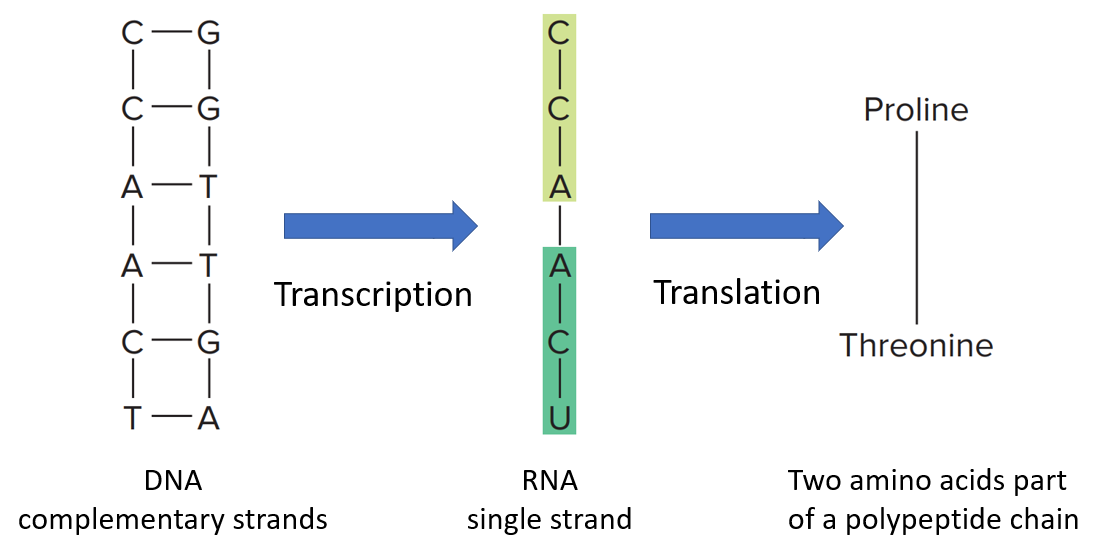
\includegraphics[width=.75\linewidth]{images/ch_2_protein_generation.PNG}
  \captionof{figure}{Conversion of DNA information into protein via the genetic code. Complementary bases in a DNA strand are split into a single RNA strand, which is read in pairs of three bases at a time (codon) to create a single amino acid in a polypeptide chain. Adapted from \cite{hartwell2008genetics}.}
  \label{fig:ch_2_protein_generation}
\end{figure}


Genes are long segments of DNA that encode information for a specific protein, and are the basic building blocks of all organisms. Proteins are made up of long chains of amino acids where the structure and function of the proteins are determined by the order of these amino acids. Proteins are manufactured using the information encoded in a gene through a process of transcription and translation called gene expression. During transcription, the DNA present in a gene acts as a template to form an mRNA (messenger RNA) structure, which is a single-stranded structure consisting of one of every complementary base pair in the DNA. This is followed by translation where mRNA is used as a template to assemble a chain of amino acids such that each group of three bases in the mRNA (called a codon) creates one particular amino acid, as shown in Figure \ref{fig:ch_2_protein_generation}. Thus the order of bases in the DNA encodes for the order of amino acids in the protein and, in turn, the protein's structure and function\cite{clancy2008translation}.

DNA is transferred from one generation to the next in all livings organisms through the process of self-replication where the double-helix structure of the DNA comes apart, and each of the complementary strands acts as a template in the production of its counterpart forming new pairs of DNA strands\cite{pray2008semi}. Although cellular error-checking mechanisms ensure that these new DNA strands are nearly identical to the original strand, mutations can occasionally occur. This can happen when a base at one position is replaced by one of the other bases or is entirely lost. Alternatively, insertions or duplications of extended sets of base pairs can also happen. Other kinds of larger mutations such as chromosomal rearrangements can also occur, including inversions (where a large segment of a chromosome is inverted in orientation) or translocation (where parts of chromosomes swap places)\cite{hartwell2008genetics}. While most mutations that occur during duplication do not have an effect on a gene, they can occasionally alter the gene's function. This can be detrimental, leading to diseases such as cancer in certain cases. Alternatively, such mutations can also be beneficial by offering resistance to diseases or other environmental stresses. 

\subsection{Comparative Genomics}\label{comparegenomics}

As mutations accumulate over time, they lead to the divergence of species. Understanding how these changes could have occurred is a significant area of study in comparative genomics and has large scale implications such as discerning the role of genetic factors in human health and disease\cite{collins2003vision}. Comparative genomics, as the name suggests, involves comparing genome sequences of different species to identify regions of similarity and difference in order to gain information about the relatedness between the species genomically and functionally. The fundamental principle in comparative genomics remains simple in that sequences that encode for proteins and gene expression should be conserved in related species, whereas sequences that are responsible for differences between species will themselves be divergent\cite{hardison2003comparative}.

Comparative genomics can assist biologists in linking the phenotypic and genotypic properties of an organism to understand its different characteristics. For example, researchers combined the gene expression data of several plant sequences which have high gene duplication rates with evolutionary conservation data to improve gene discovery \cite{hanada2008importance}. Also, the comparative analysis of genes and their regulatory pathways in the context of phylogeny (the study of evolutionary relationships) provides scientists with a better understanding of how evolution happens at the molecular level\cite{soltis2003role}. However, the questions that are addressed by comparing genomes at different phylogenetic distances can vary \cite{hardison2003comparative}. For example, genomic comparison between species that are separated by very long phylogenetic differences such as yeast (\textit{Saccharomyces cerevisiae}), worms (\textit{Caenorhabditis
elegans}), and fruit flies (\textit{Drosophila melanogaster}) reveals that their genomes encode for many of the same proteins while the order of the genes and sequences are not conserved\cite{rubin2000comparative}. In contrast, comparison between more closely related species like Humans (\textit{Homo sapiens}) and Chimpanzees (\textit{Pan troglodytes}) reveal that the overall divergence between the two genomes is only 4\% and results are more oriented towards identifying the differences than the similarities \cite{varki2005comparing}. 

Comparative genomic studies are primarily focused around the study of homologous sequences, which are gene sequences that have shared ancestry. The extent of homology is determined by sequence similarity and such similar sequences are commonly referred to as homologs. Such similarity between DNA sequences of two different species can occur either because of a speciation event (a species diverges into two separate species) leading to orthologs, or due to a gene duplication event (a gene is duplicated within the same genome) leading to paralogs \cite{jensen2001orthologs}. Research into such similar genes, especially in eukaryotic organisms, can shed light on gene duplication events that led to the creation of gene families\cite{rubin2000comparative}. Gene families are defined as large groups of gene sequences that are similar to each other while also having a similar function or gene expression. Usually, when a gene duplication occurs the new gene either becomes inactive as a pseudogene or exists as a duplicate copy of the original gene performing the same function. An increased number of gene duplicates through natural selection can often lead to an increase in the protein synthesized by the gene. An example of this is the variation in gene copy number in the human salivary amylase gene (AMY1) responsible for starch hydrolysis in certain human populations\cite{perry2007diet}. A third scenario of gene duplication that occurs rarely is when the duplicated gene acquires a new function through mutations. An example of this is the trocarin D gene of the Australian rough-scaled snake that acts as a toxin by coagulating the blood of its prey. Comparative genomic analysis of the trocarin D gene revealed that it is nearly identical to the coagulation factor X gene present in the plasma of the snake responsible for blood coagulation (to prevent bleeding when injured) indicating that that the gene was recruited for a new function after a gene duplication event\cite{reza2007structure}.

\subsection{Synteny}
One of the ways in which homology can be inferred for understanding large scale duplication events is through studying collinearity of several genes, where both the gene content and order are conserved\cite{proost2011adhore}. Such long regions containing several genes that display collinearity in the order of kilobases (Kbase) to megabases (Mbase) are referred to as \textit{synteny blocks}\cite{zeng2008orthocluster}. The word synteny has Greek origins with \textit{syn} meaning ``together'' and \textit{taenia} meaning ``ribbon'' and is used to indicate the presence of genetic loci on the same chromosome\cite{renwick1971mapping}. However, synteny can also occur between different chromosomes and the term is more commonly used to refer to ``gene loci in different organisms located on a chromosomal region of common evolutionary ancestry''\cite{passarge1999incorrect}.

With the availability of fully sequenced genomes for several model species, synteny analysis can reveal evolutionary adaptions and also improve the transfer of knowledge to non-model organisms that have not been fully mapped\cite{zhao2019network}. Synteny analysis, particularly in angiosperms (flowering plants), can help in understanding the consequences of whole genome duplication in plant evolution\cite{adams2005polyploidy} as shown in the analysis of polyploidy in Thale cress (\textit{Arabidopsis thaliana}), which despite its relatively small genome size has been shown to have undergone repeated cyclical genome doubling \cite{seoighe2004genome,seoighe2003turning}. This state of polyploidy where an organism contains more than two sets of homologs is a widespread occurrence in plants  due to several whole-genome duplication events at diverse temporal scales but is rare in mammals with evidence of the last whole genome duplication event occurring almost 500 million years ago\cite{adams2005polyploidy,panopoulou2005timing}. The increase in genome size due to polyploidy can occur either due to the inheritance of duplicated sets of chromosomes from the same species where its called autopolyploidy, or due to hybridization between two difference species where its referred to as allopolyploidy. Such changes in genome structure can often have immediate effect on the phenotype and fitness of the individual and in certain hybridization scenarios can even improve the ``vigor'' of the resultant polyploid compared to its parental species \cite{otto2007evolutionary}. Synteny analysis of the genomic structure of such polyploid individuals can assist researchers in predicting the number and timings of polyploid events in the organism's evolutionary history \cite{adams2005polyploidy}. 

While polyploidy in the form of whole genome duplication continues to be a driving factor in the evolution of plants, genomes of mammals show evidence of only two shared rounds of whole genome duplication specified in the 2R hypothesis \cite{hokamp20032r}. However gene collinearity is conserved to a greater degree in mammals than plants thus making synteny analysis at smaller scales (called microsynteny) much more feasible\cite{zhao2019network}. In this way, synteny analysis can be adapted to a wide range of genomic scales based on the underlying question.

\begin{figure}[h]
  \centering
  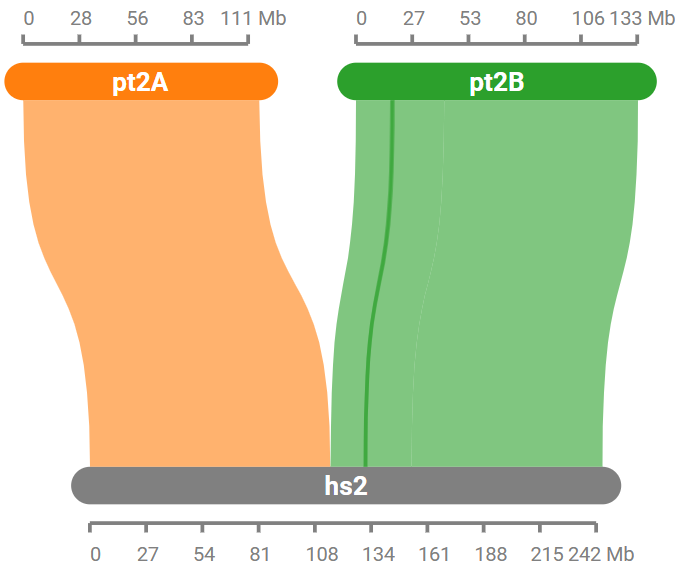
\includegraphics[width=.35\linewidth]{images/ch_2_fission.PNG}
  \captionof{figure}{Synteny between chromosomes 2A and 2B from Chimpanzees (\textit{Pan troglodytes}) and chromosome 2 from Humans (\textit{Homo sapiens}) depicting an ancestral chromosomal fission event.}
  \label{fig:ch_2_fission}
\end{figure}

Apart from regular duplication events mapping syntenic regions can also help in identifying other genomic rearrangement events such as fusions, fissions, translocations, inversions, and deletions \cite{wei2002comparative,o1999promise}. Chromosomal fusion can occur at both the telomeres (ends of a chromosome) or centromeres (center of a chromosome linking two chromatids) and is caused by the union of two or more chromosomes to form a single entity. Human chromosome 2 is a well known example of ancestral telomere-telomere fusion of two ape chromosomes as shown in Figure \ref{fig:ch_2_fission} \cite{ijdo1991origin}. Similarly fission is the splitting of two functional halves of a chromosome where the break point is usually situated at the centromere (centric fission) \cite{rieger2012glossary}. This can lead to an increase in chromosome number and in certain instances such as the model species of yellow monkey-flowers (\textit{Mimulus guttatus}) synteny analysis has shown that multiple centric fission events (along with partial fusion) provide a better explanation for near-doubling of chromosome numbers compared to the traditional whole genome duplication theory \cite{fishman2014comparative}. 

\begin{figure}[ht]
  \centering
  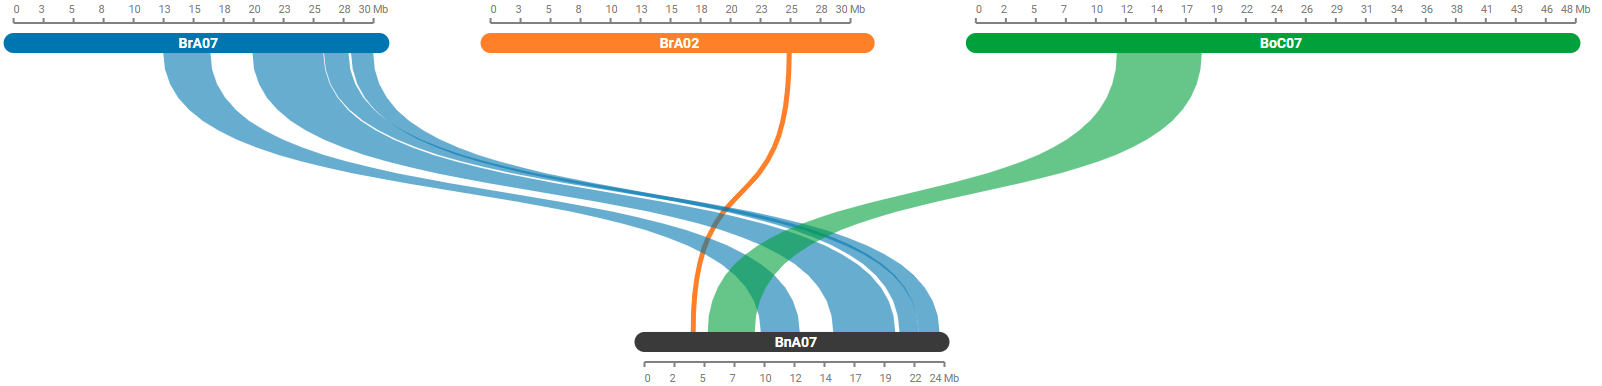
\includegraphics[width=.95\linewidth]{images/ch_2_complex.PNG}
  \captionof{figure}{Synteny between \textit{Brassica napus} and its ancestors \textit{B. rapa} and \textit{B. oleracea} showing reciprocal translocation rearrangements.}
  \label{fig:ch_2_complex}
\end{figure}


Another common type of chromosomal rearrangement is translocation which is caused by the change in the position of segments of a chromosome. These variations can be either intrachromosomal or interchromosomal. The former is a type of variation where segments are shifted from one arm of a chromosome to the other and the later occurs when  a segment is transferred from one chromosome into another (transposition) or segments are mutually exchanged between different chromosomes (reciprocal) \cite{rieger2012glossary}. In certain scenarios both intra and interchromosomal translocations can occur together. An example of this can be seen in the synteny analysis of \textit{Brassica napus} an allotetraploid containing the A-genome and C-genome from its progenitor species of \textit{B. rapa} and \textit{B. oleracea}. While 8 chromosomes were found to contain only skeletons from the corresponding chromosomes of B. rapa or B. oleracea, 11 others were composed of different chromosomal segments along with the skeletons indicating that a variety of chromosomal rearrangement events occurred after the initial duplication \cite{parkin2003patterns,cai2014complex}. If we look at chromosome BnA07 in \textit{B. napus} as shown in Figure \ref{fig:ch_2_complex}, it consists of three different chromosomal sources. The first is the skeleton of BrA07 from \textit{B.rapa}, the second is a fragment of BrA02 from \textit{ B.rapa} that occurred through reciprocal translocation and, the third is a homologous fragment of BOC07 from \textit{B. oleracea}. Finally inversions and deletions are two other types of genomic rearrangements where the former occurs when a segment of a chromosome is reversed in orientation and put back in its place and the later occurs when a portion of chromosome is lost \cite{rieger2012glossary}. An example of inversion can be seen in the comparitive mapping of \textit{Lens culinaris} and model legume \textit{Medicago trunctula}, where a large set of inversions (colored red in Figure \ref{fig:ch_2_inversions} (left)) are shown between chromosome 1 of \textit{L. culinaris} relative to chromosome 1 of \textit{M. truntula} \cite{gujaria2014genetic}. These inversions are much more evident in dot plots (Figure \ref{fig:ch_2_inversions} (left)) as they show up as perpendicular lines to the diagonal. In this way apart from the study of polyploidy, synteny analysis can also be used in understanding different kinds of chromosomal rearrangements.

\begin{figure}
  \centering
  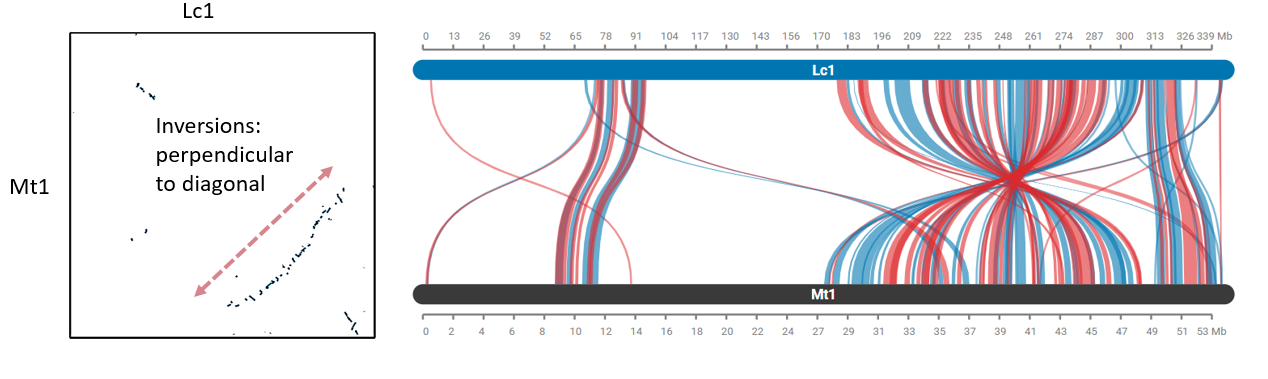
\includegraphics[width=.99\linewidth]{images/ch_2_inversions.PNG}
  \captionof{figure}{Synteny mapping between Chromosome 1 from \textit{L. culinaris} and \textit{M. truntula} showing large scale inversions through a dot plot (left) and a parallel plot (right). The red ribbons represent inverted syntenic regions and the blue ribbons represent regular regions.}
  \label{fig:ch_2_inversions}
\end{figure}

\subsection{Analysis Pipeline}

Synteny analysis consists of three major steps: sequence alignment, synteny detection, and data visualization. Although SynVisio focuses on the last step, we will take a brief look at the other preceding steps. Before analyzing synteny between organisms their genomes need to be sequenced and assembled at least partially into scaffolds. This process is then followed by similarity detection between the two genomes through sequence alignment.



\subsubsection{Sequence Alignment}
Sequence alignment is extensively used in computational biology to assess the similarity between DNA, RNA, and protein sequences. Sequence alignment works by arriving at an optimal alignment through a scoring mechanism, where gaps are introduced in one or both of the sequences but penalized accordingly, as shown in Figure \ref{fig:ch_2_sequence_alignment_multi}. A gap at any position in the final alignment is an indication of an insertion or a deletion and is penalized because these events are far less likely to occur than mutations. The validity of sequence alignment results is dependent on the alphabet size of the sequences; protein sequences can contain up to 20 different amino acids, whereas DNA sequences only contain four different bases, leading to better alignments in proteins. There are two major types of sequence alignments, and they are each used in different scenarios. The first type of sequence alignment is called a global sequence alignment, where an optimal match is found by aligning the two entire sequences end to end, and is used to compare homologous sequences. The second type of alignment that looks at smaller sections or sub-sequences is called local sequence alignment and is used to look for patterns in a sequence when comparing it with a larger set of sequences such as those in a database. 

\begin{figure}
  \centering
  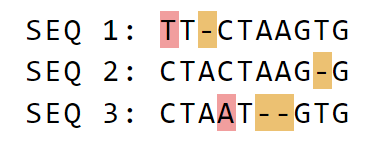
\includegraphics[width=.45\linewidth]{images/ch_2_sequence_alignment_multi.PNG}
  \captionof{figure}{Sequence alignment of sequences `TTCTAAGTG',`CTACTAAGG' and `CTAATGTG' with mismatches and gaps highlighted in red and orange.}
  \label{fig:ch_2_sequence_alignment_multi}
\end{figure}


Every sequence alignment is centred around an optimization problem and early alignment techniques such as the Needleman and Wunsch method \cite{needleman1970general} used a dynamic programming approach to arrive at the optimal alignment. Dynamic programming is a computational strategy that recursively breaks larger problems into smaller sub-problems and reuses the results of previously solved sub-problems to arrive at a solution to the larger problem. A variation of the Needleman and Wunsch method for local sequence alignment is the Smith-Waterman algorithm\cite{smith1981identification} that uses a matrix-based scoring scheme for comparing sub sequences.
However, the time complexity of such methods is exponential meaning that searching for sequences in large databases is infeasible. This has led to the adoption of heuristic methods to align sequences such as the FASTA (Fast-All) algorithm \cite{lipman1985rapid}. Although this algorithm is no longer in use, the name FASTA is still used for a popular file format in bioinformatics, that represents nucleotide and protein sequences as a series of single-letter characters.

BLAST (Basic Local Alignment Search Tool) is a popular local sequence alignment tool that acts as a direct successor to the FASTA algorithm, being more time-efficient and operating on the same file format\cite{pertsemlidis2001having}. It operates by identifying small query words that contain three nucleotides or amino acids for protein sequences in a particular order based on their occurrence along the sequence and closeness to other similar words. It then expands on these words in  either direction based on searches from target databases that are rated by a special scoring matrix. BLAST by default uses BLOSUM62 (Block Substitution Matrix) as its scoring matrix which ensures that even more distantly related sequences are detected, but other matrices such as PAM250 (Point Accepted Mutation) can also be specified.



\subsubsection{Synteny Detection Tools}

The next step after detecting the similarity between two sequences is the actual synteny detection, as alignment results are only pairwise between sequences and need to be grouped into larger blocks to look for patterns. Although synteny detection tools differ in their operating file formats and computational efficiency, they broadly work by combining positional information of genes along a genome sequence with pairwise BLAST results to construct chains of collinear gene pairs. Grouping neighboring gene pairs that match is one way of detecting syteny\cite{wang2012mcscanx} that is implemented in tools such as OrthoCluster\cite{zeng2008orthocluster}, TEAM\cite{luc2003gene} and ADHoRe\cite{proost2011adhore}. These tools are, however, outdated and are not efficient in detecting syntenic blocks with conserved gene order, especially in scenarios that might include chromosomal rearrangements and tandem duplications\cite{wang2012mcscanx}. A new class of synteny tools such as MCScanX\cite{wang2012mcscanx}, DAGChainer\cite{haas2004dagchainer}, and CYNTENATOR\cite{rodelsperger2010cyntenator}, that utilize a dynamic programming approach to create chains of pairwise collinear genes around anchor genes are much more efficient at detecting collinear syntenic blocks. Some tools such as MCScanX even offer downstream analysis tools with static visualization results, as shown in Figure \ref{fig:ch_2_synteny_plots}.     

\begin{figure}
  \centering
  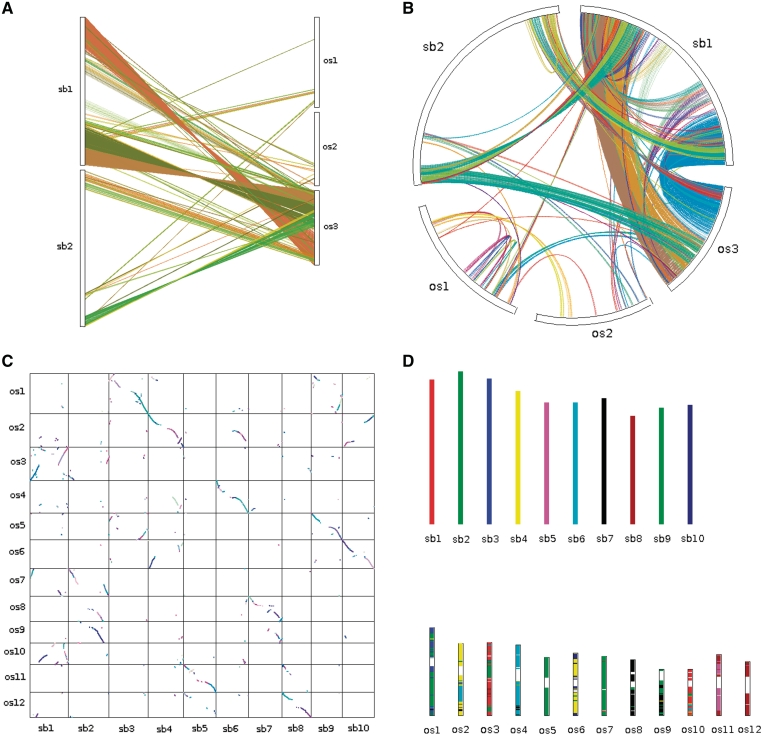
\includegraphics[width=.75\linewidth]{images/ch_2_synteny_plots.jpg}
  \captionof{figure}{Different types of plots visualizing synteny generated by MCScanX : (A) dual synteny plot, (B) circle plot, (C) dot plot and (D) bar plot, From Wang et al.\cite{wang2012mcscanx}.}
  \label{fig:ch_2_synteny_plots}
\end{figure}

\section{Genomic Visualizations} 
With the advent of rapid genome sequencing systems, genomic data is being generated at a rapid pace that is not being equalled in terms of innovations in data analysis systems that can help researchers in understanding these ever-increasing data streams. Visualization systems can play a critical role in bridging this gap in data exploration as humans are intuitively good at finding visual patterns. As research in this field becomes increasingly data-driven, visualization systems can aid researchers in generating a hypothesis and iteratively refining it by encoding genomic information through visual cues in the form of shapes and colours\cite{nusrat2019tasks}. Genomic visualization systems can be used in several scenarios, such as analyzing sequence data at different resolutions and browsing annotations and reference tracks or in comparing sequences from different organisms\cite{nielsen2010visualizing}. However a major challenge in this field remains in determining the right graphical representation based on the genomic context and data under exploration. In this section, we first explore the different kinds of visualizations systems and techniques that are used in representing genomic data at the sequence and genome level. We then look at systems that are used in exploring sequence similarity at different resolutions and finally give a brief overview of current synteny visualization systems and their merits and limitations.

\subsection{Sequence and Genome Browsers}
Visualizing genomes at the sequence level is primarily done by representing sequences
as a series of letters organized on a linear scale from left to right. Additionally, sequences that are longer are stacked vertically in a scrolling window. This ordering of bases or amino acids is meant to aid researchers in identifying discrepancies by quickly scanning down the sequence along its length, especially in scenarios involving comparison of read alignments. Visual cues such as emphasis through colours are further used to highlight erroneous bases in some sequence analysis tools\cite{consed,ewing1998base}. Other tools like IGV (Integrative Genomics Viewer)\cite{thorvaldsdottir2013integrative} and Hawkeye\cite{schatz2007hawkeye} opt for a simpler representation by only visualizing discrepancies. Sequence visualization systems are also used to interpret and refine the results of sequencing systems where visual cues are provided to highlight gaps, mismatches, and the order of repeats\cite{bonfield1995new,consed}. In some systems such as Consed\cite{consed}, information is visualized in pairs that are colour-coded so that structural variations such as insertions, deletions, and inversions are also considered, and additional information is provided in the form of annotations of amino acid translations to identify mis-assemblies. Finally, some tools like the ABySS-Explorer provide an assembly graph overview for high-level inspection of the assembly instead of focusing on the local sequence mismatches\cite{nielsen2009abyss}. 


\begin{figure}
  \centering
  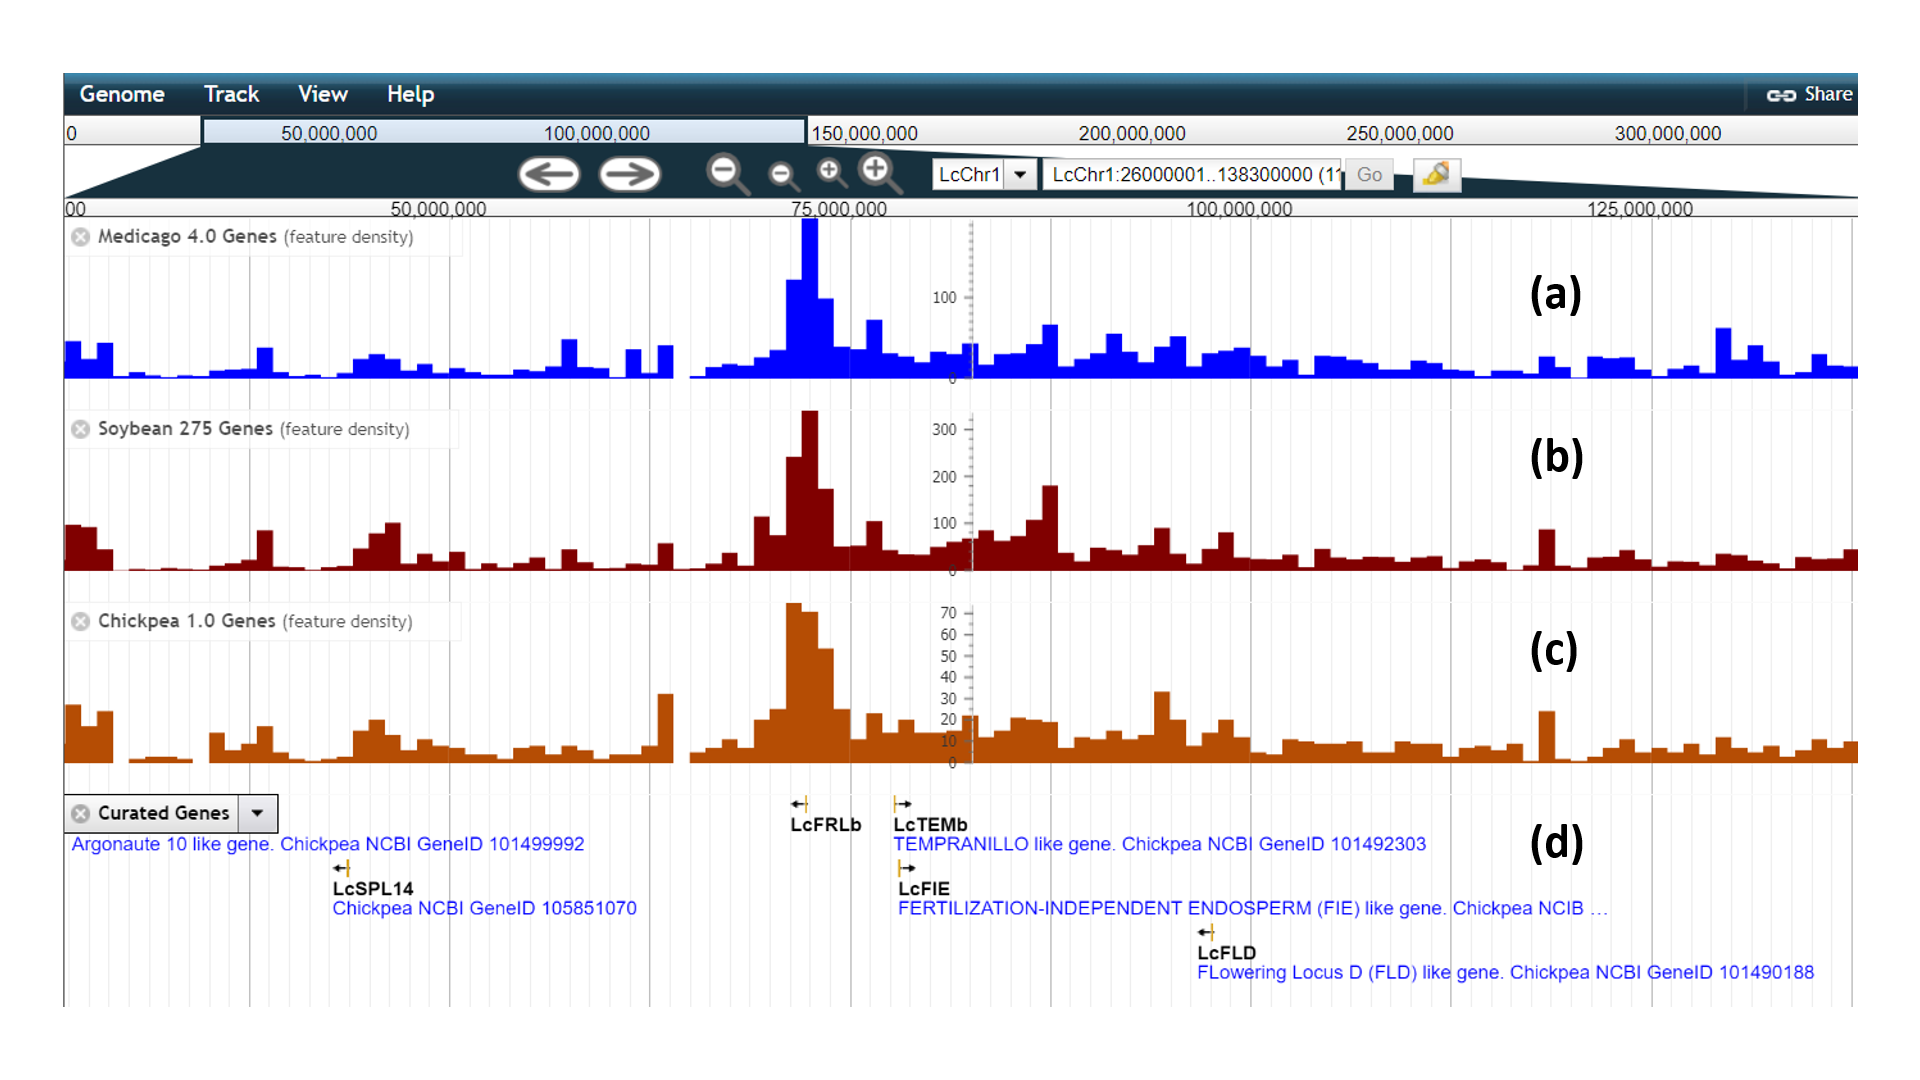
\includegraphics[width=1\linewidth]{images/ch_2_jbrowse.PNG}
  \captionof{figure}{JBrowse is used to compare gene densities between (a) Barrel Medic (\textit{Medicago truncatula}), (b) Soybean (\textit{Glycine max}) and (c) Chickpea (\textit{Cicer arietinum}) in relation to a set of curated genes encoding for prominent phenotypes (d) generated through KnowPulse \cite{sanderson2019knowpulse}. }
  \label{fig:ch_2_jbrowse}
\end{figure}


Once the short sequence reads are assembled into a single large genome, a different set of visualization tools are required that are focused around identifying particular regions of interest. A genome sequence in its entirety can act as a reference against which several features such as gene densities, SNPs, and repeats can be mapped. This form of analysis is increasingly being used in a wide range of browsers that were developed to disseminate information and provide a platform for the exploration of several genomes that are sequenced for model organisms. These tools include GBrowse\cite{stein2002generic}, Ensembl Genome Browser\cite{stalker2004ensembl} and UCSC Genome Browser\cite{ucscgenome}. These browsers work by displaying a requested portion of the genome with several annotation tracks stacked in rows vertically along a reference axis. The annotation tracks can contain different kinds of information such as positions of single nucleotide polymorphisms, regions with regulatory elements, or location of important genes, as shown in Figure \ref{fig:ch_2_jbrowse} (d) and can be toggled on or off depending on their role in the analysis. The information is visualized at several resolutions from hundreds of base pairs all the way up to tens of thousands with the ability to move along the genome horizontally and zoom in and out of a particular region. Some genome browsers even offer the ability to search for a particular gene by looking up its position in the underlying database\cite{nielsen2010visualizing}. 

Finally, additional visual representations such as summary views (e.g. copy number variations) in the context of biological pathways are also provided in certain browsers like UCSC Cancer genomics browser\cite{ucscgenome}, allowing researchers to associate clinical features with genomic data directly. This form of a genome overview that preserves global context while still allowing researchers to explore smaller chromosome level entities is also present in Gremlin, a tool that offers a novel visual model for exploring structural variants and rearrangements\cite{o2010gremlin}.  

With an increase in the volume of data being generated, genome browsers are beginning to use a decentralized model where processing power is distributed between the server and the client's browser. Information is retrieved only when needed for the region that the user is interested in, and visualizations are generated dynamically at the client-side. This reduces the load on the server substantially and modifies it to serve purely as a database to look up information when necessary. This form of rendering in the client can offer a smoother interactive experience while navigating a genome through panning or zooming. It also ensures that there are no disruptions to a user's sense of location, by averting incongruous transitions that occur when large data sets are being loaded and traversed. An example of this approach is JBrowse, which offers visualizations as shown in Figure \ref{fig:ch_2_jbrowse}, along with significantly reduced server overhead compared to other genome browsers\cite{skinner2009jbrowse}.
Certain genome browsers take this decentralized model a step further by offering connectivity to data stored locally on a user's computer\cite{ucscgenome,saito2009utgb}. This can provide a personalized experience when dealing with sensitive data in situations where storing data on a remote server may not be viable. 

\subsection{Comparative Genome Browsers}
With the ability to sequence multiple genomes within a short span of time, a new field of research has emerged that focuses on comparing genomes instead of looking at them in isolation; this field is called comparative genomics, as discussed earlier in Section \ref{comparegenomics}. Regardless of the data type or domain, comparison is a common task in data analysis and visualization, when there is a need to understand the relationship between a given set of items.\cite{gleicher2017considerations}. Visual comparison has been shown to improve the understanding of data in several charts and designs explored by Tufte\cite{tufte1990envisioning} along with specific examples centred around Playfair's use of line graphs to demonstrate the change in stock prices in relation to wars\cite{costigan1990william}. In the field of genomics, comparison can aid biologists in a diverse set of tasks such as identifying functional elements, studying large scale rearrangements and genome evolution, and refining results of genome assembly systems through reference genomes\cite{nielsen2010visualizing}. Several systems have been built to address each of these tasks through visual comparison at different genomic scales as sequences can be compared at the nucleotide level all the way up to the whole genome level.

At the nucleotide level, researchers compare sequences to identify the location of mutations, insertions, and deletions; most visualization tools designed for such analysis achieve this by representing alignments on a linear scale. Visual cues are provided by colouring each of the four nucleotides with a categorical colour scale, and the sequences are presented in a linear layout, usually in a stacked arrangement. Some of these tools, such as JalView (JV2)\cite{waterhouse2009jalview}, are enhanced with interactive features that let users sort, filter, highlight, and edit multiple sequences in real time. Jalview also lets users overlay sequence features onto the alignment and render extra positional features through transparent or opaque shading over specific regions of an alignment. AliView is a similar tool that works for extremely large datasets through an indexing process and offers support for multiple file formats\cite{larsson2014aliview}. JalView and AliView, however, are limited in usability being desktop applications but recent tools such as MSAViewer\cite{yachdav2016msaviewer} and JSAV (JavaScript Sequence Alignment Viewer)\cite{martin2014viewing} have been designed to work across the internet as web applications with a similar set of features.

When comparing sequences at higher levels, researchers look for large scale rearrangements. Due to the higher resolution of data, genomic features are grouped into contiguous blocks on each chromosome called syntenic blocks where conservation is implied through the similarity and relatedness between these blocks.
Several strategies have been explored to graphically represent syntenic blocks both at the chromosome and the whole genome level. The earliest examples for representing synteny involve the adaptation of dot plots used for comparing local alignments for larger sequences. Most of these tools primarily perform the actual genome level comparison and present their results through dot plots for closer inspection such as DAGChainer\cite{haas2004dagchainer} or the VISTA plots of the MUMmer alignment tool\cite{kurtz2004versatile}. Dot plots are two dimensional representations where genomes of two organisms are presented along the \textit{x} and \textit{y} axes. Gridlines are used to show chromosomal boundaries, and every similar gene is represented as a point, implying that large collinear blocks of genes are shown as lines. Such matrix-based representations are extremely good at identifying genome rearrangements, as duplications show up as secondary lines parallel to the diagonal and inversions end up as straight lines that are perpendicular or inclined away from the diagonal. While these plots offer effective genome level summaries of alignments, they cannot be extended for multi-way comparisons between several genomes or used to identify smaller rearrangements at the chromosome level.

\begin{figure}
  \centering
  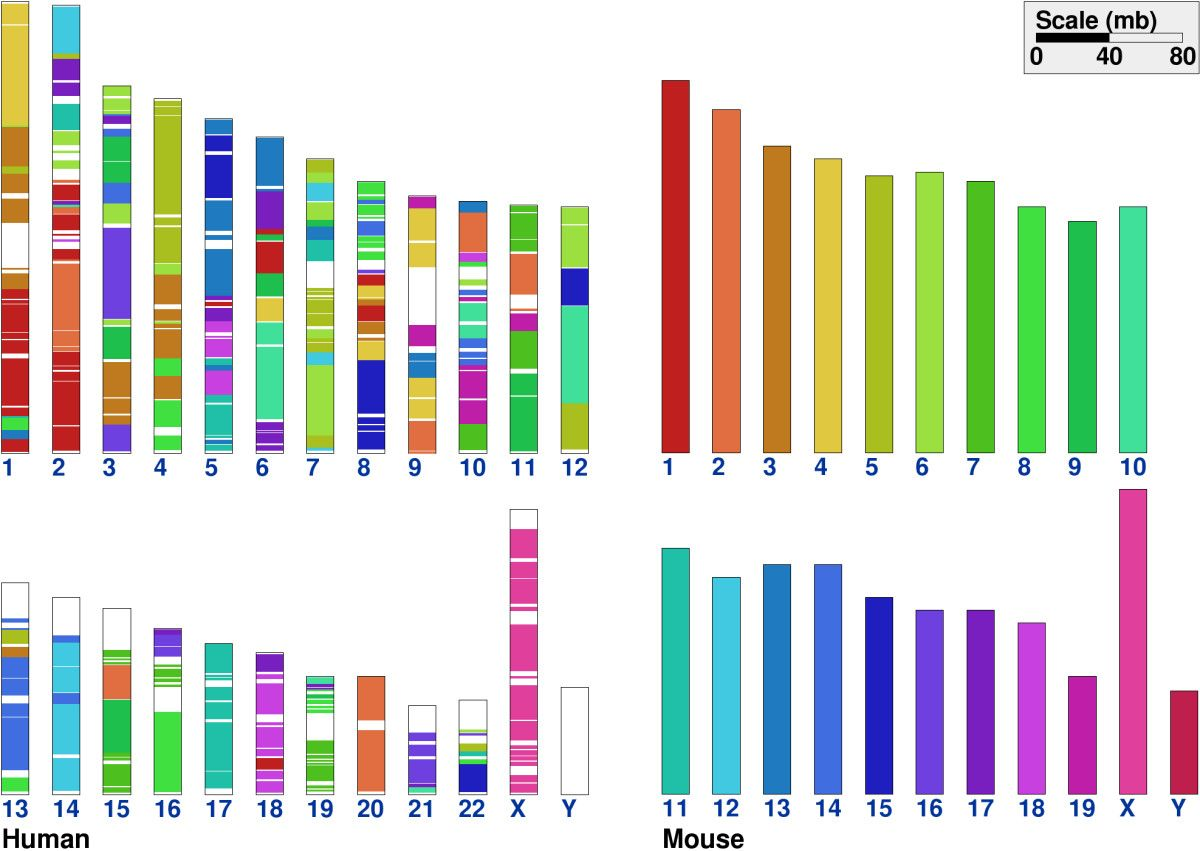
\includegraphics[width=0.75\linewidth]{images/ch_2_cinteny_pill.jpg}
  \captionof{figure}{Visualization of synteny between human and mouse genomes shown by a pill-based design in Cinteny. Image extracted from \cite{sinha2007cinteny}. }
  \label{fig:ch_2_cinteny_pill}
\end{figure}

Another representation of synteny that has been used extensively in tools such as Cinteny\cite{sinha2007cinteny}, Sybil\cite{crabtree2007sybil} and MEDEA\cite{nusrat2019tasks} is the pill-shaped ideogram design of chromosomes. In this design, chromosomes of the source genome are represented as pill-shaped rectangular blocks that are colour coded on a categorical scale and chromosomes in the target block are represented as similar pills with varying sizes based on their genomic sizes. Syntenic regions in the target are then represented through colour coded bands where the colour is determined by the source chromosome that the alignment belongs to, as shown in Figure \ref{fig:ch_2_cinteny_pill}.
The choice of representing a chromosome as a rectangular pill is based on a karyogram representation often used for chromosomes in biological literature\cite{pearson1973uniqueness}, but information about the position of the centromere is omitted, and the ``X" or ``V" shaped design is adopted into a single cylinder shaped like a small pill. While the use of colours makes it easier to quickly identify similar regions and their distribution in the target genome in comparison to a dot plot, this representation loses some information such as the orientation of the aligned blocks and their relative position in the source genome. Tools like Apollo partially solve this problem by extending the representation by also linking the coloured segments in the reference genome with their corresponding loci in source chromosome through lines, and by interleaving the source and target regions \cite{lee2009apollo}. Mauve follows a similar approach but uses a linear layout and stacks the sequences parallel to each other, using connections to encode conservation\cite{darling2004mauve}. A significant problem with this representation, along with other designs that rely extensively on colour is that it cannot be extended for a large number of chromosomes as humans cannot intuitively distinguish beyond ten colours \cite{tufte1990envisioning}. Further, the choice of colours is extremely important as colours need to be visually distinct unlike the colours chosen in tools like Cinteny\cite{sinha2007cinteny} as shown in Figure 2.5. The colours used in chromosomes 6-9 and 12-15 are very close to each other in the green and blue spectrum and it is hard to distinguish them when the coloured bands in the target are small and close to each other. 

A third form of representation that has recently become popular due to its aesthetic appeal is the Circos style plot\cite{krzywinski2009circos}. In these plots, genomes are represented as arcs presented in a circular layout. Syntenic regions are shown as lines connected through the middle of the circle. Additional tracks representing other information such as copy number variants and SNPs are presented through outer circles along the genome. The circular arrangement is meant to reduce visual clutter that can arise in a linear stacked arrangement when multiple linked regions are represented through connections that cross each other excessively. Tools like Circa that generate these plots can be configured to use a diverse set of colour schemes and visual representations like histograms, heat maps, line charts, and scatter plots for the outer tracks\cite{circa}. 

\begin{figure}
  \centering
  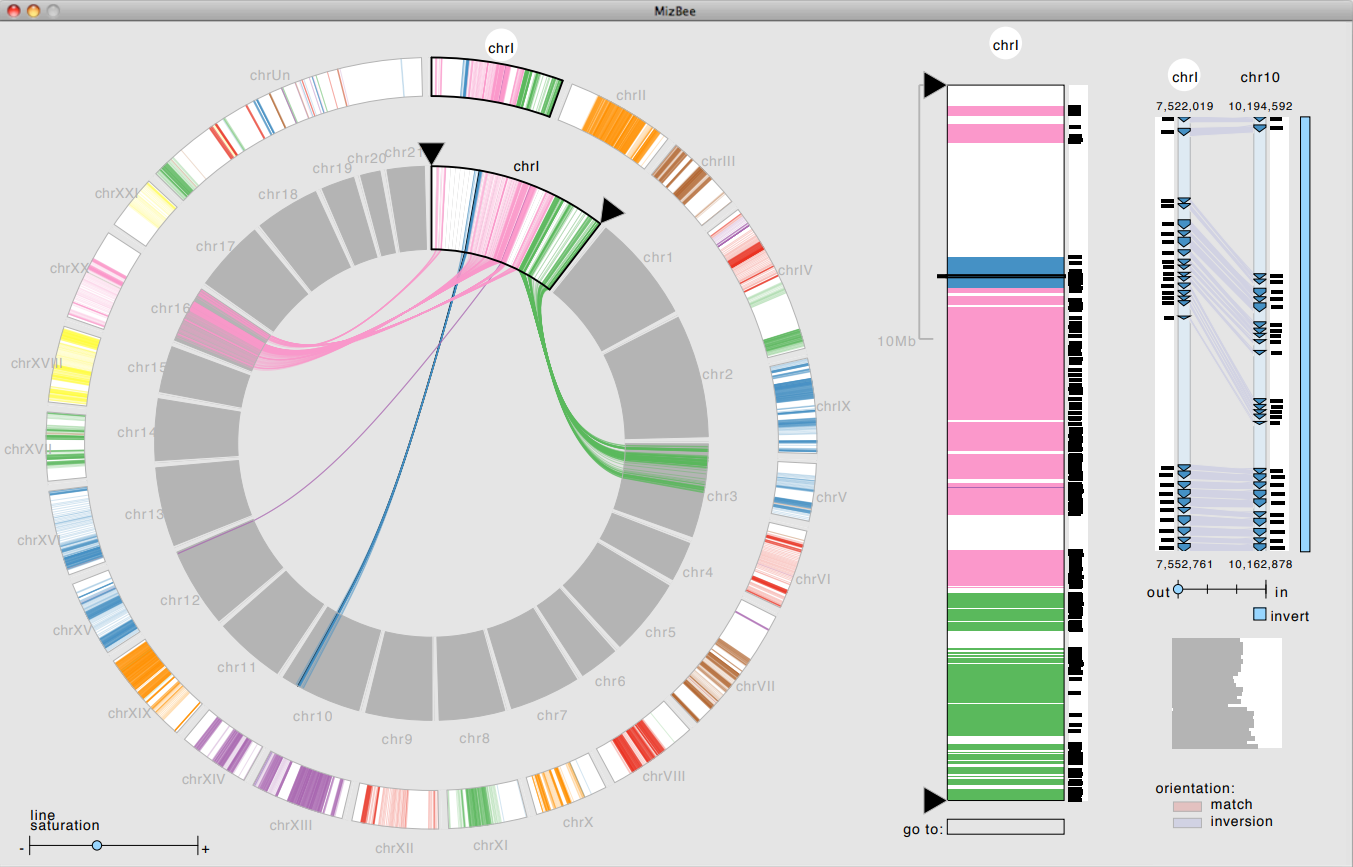
\includegraphics[width=0.75\linewidth]{images/ch_2_mizbee.PNG}
  \captionof{figure}{Synteny visualization as shown by Mizbee. Image extracted from \cite{Meyer2009}. }
  \label{fig:ch_2_mizbee}
\end{figure}

Mizbee is an example of a standalone synteny browser that combines the circular layout with a linear arrangement to present syntenic information at different scales. Mizbee presents genomic conservation through a combination of connections and colour encoding in three linked views that are presented next to each other, as shown in Figure \ref{fig:ch_2_mizbee}. In the genome view, chromosomes are presented as arcs in two concentric rings. The source chromosomes are presented in the outer ring, and the inner ring contains the target chromosomes arranged around a copy of the selected source chromosome. Conservation is then encoded through links connecting the collinear blocks inside the inner ring with additional encoding in the form of colour. The circular layout reduces visual clutter, which is further addressed through edge bundling of contiguous blocks\cite{zhou2013edge} that go to the same destination chromosome. Data in the inner ring can be explored by selecting a particular region which is then presented in a chromosome view in the middle of the display, as seen in Figure \ref{fig:ch_2_mizbee}. The colour coding at this level is similar to the genome view but connections are presented in a vertical layout that supports precise spatial analysis. The final view, called the block view, presents the individual genes in a particular collinear block through connected ribbons along with their orientation encoded as directed triangular blocks. Mizbee is the first of many browsers that have been developed to go beyond simple chart generation and act as a complex analysis tool that can present conservation through a combination of multiple visual representations. Mizbee, however, doesn't perform the actual synteny detection and relies on a formatted input dataset. This requires researchers to first detect synteny through a detection tool like DAGChainer, MCScanX or iADHoRe and then modify the output to match the input format of Mizbee. Mizbee also doesn't supplement the generated visualizations with tracks for additional information that provide biological context, and is limited in its usability being a standalone desktop tool. 

mGSV (Multi Genome Synteny Viewer) is a synteny viewer that works similarly to Mizbee by visualizing synteny through a combination of visual representations, but is available as a web-based tool\cite{revanna2011gsv}. It lets users upload pre-computed syntenic data in a tab-delimited format and also accepts an extra annotation file to show additional genomic features as an annotation track. The system, however, works in a distributed model where syntenic information is stored in a remote database and charts are generated at the server and fetched based on user interactions in the browser. This server-based model can cause data security issues and also add unnecessary network delay into the analysis, making it a time consuming process. SimpleSynteny is another web based tool that represents information in a horizontal linear layout using a combination of coloured bars and connected ribbons for representing genomic conservation\cite{veltri2016simplesynteny}. It however accepts FASTA files as input for the genomes and uses BLAST\cite{blasttool} on a remote server to align the sequences into collinear blocks. While this does improve the usability of the tool, synteny detection is a resource intensive process that can place a heavy load on the server, especially for large genomes, and is best done on desktop machines that are computationally powerful.

A recent set of synteny browsers that are web based and also let users download visualizations as image files are Synteny Portal, MultiSyn, and AccuSyn. Synteny Portal uses alignments that are pre-built and stored in the UCSC genome browser database but cannot be extended for custom sequences\cite{lee2016syntenyportal}. MultiSyn\cite{baek2016multisyn} is similar to SimpleSynteny but relies on only protein sequences as its input and detects synteny on the server using MCScanX\cite{wang2012mcscanx}, a popular synteny detection tool. AccuSyn\cite{accusyn} is a recent tool that lets users upload synteny results of MCScanX and generates visualizations in real-time on the client. It presents conservation similar to Mizbee in two linked views with a Circos style layout with connected ribbons for the genome level and a vertical layout with connected glyphs for the block level, as shown in Figure \ref{fig:ch_2_accusyn}. AccuSyn also lets users upload several annotation tracks with the ability to customize the colour scale and the visual representation of the track. Finally, AccuSyn attempts to minimize overlaps in the connecting lines by rearranging the chromosomes with a simulated annealing algorithm.

\section{Interaction Techniques in Genomic Visualizations}
Visualization for data exploration and analysis primarily involves graphical representation of the data, but user interaction still plays a major role in both navigation and assessment of the generated visualizations.  In this section, we first explore the different techniques that are used in genomic visualization tools to manipulate both the underlying data and the graphical interfaces for data exploration, and then discuss how data analysis can be improved with support for revisitation and tracking user interactions.

\begin{figure}
  \centering
  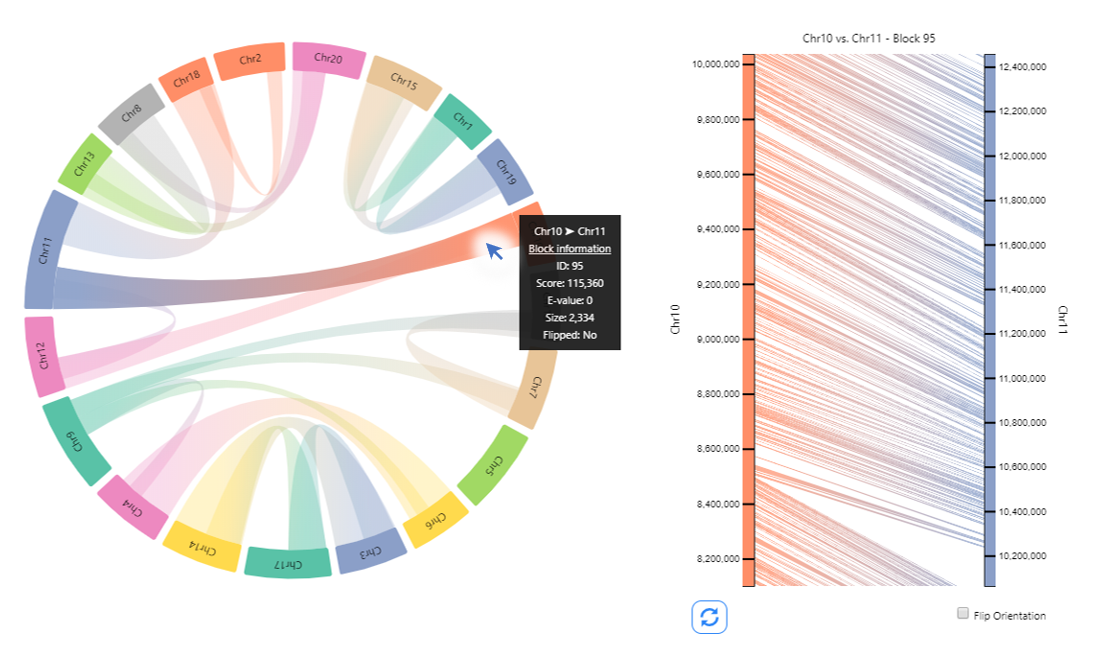
\includegraphics[width=0.95\linewidth]{images/ch_2_accusyn.PNG}
  \captionof{figure}{Multi View Synteny Exploration in AccuSyn\cite{accusyn} showing conservation in \textit{Camelina sativa} with a single collinear block highlighted between Chromosomes 10 and 11. }
  \label{fig:ch_2_accusyn}
\end{figure}


\subsection{Multiple Linked Views}

Although visual encoding of information through static visualizations can assist users in simple data analysis tasks, the usability of this approach falls short when it is utilized for complex tasks and activities\cite{tominski2015interaction,dix1998starting,pike2009science,piringer2009multi,yi2007toward,sedig2013interaction}. The efficacy of such a system can be considerably improved by providing interaction mechanisms that can modify the graphical representations based on the different tasks, users, expertise, and other contextual factors\cite{sedig2013interaction}. Complex analysis tasks go beyond basic visual perception needed for simple tasks, and often require extended cognitive processing from the user. Interaction mechanisms are important in these scenarios because engaging user actions can enhance cognitive processing\cite{sedig2013interaction}. Research has also shown that viewing the same underlying data in multiple representations can help users in forming an accurate mental model of the data\cite{larkin1987diagram,stenning1995cognitive,sedig2005designing,wang2000guidelines}.

In the context of comparative genomic visualizations, some of the earliest examples of enhancing basic charts with interaction techniques include support for zooming into a two dimensional dot plot for closer inspection of a particular region in Dagchainer\cite{haas2004dagchainer}. Tools like SynMap2\cite{haug2017synmap2} belonging to the CoGe (Comparitive Genomics)\cite{coge} web platform also allow exploration of dot plots through mouse-based scrolling and panning similar to modern mapping platforms like Google maps. This form of zooming for exploration is also used in several other tools and is part of the larger design principle proposed by Shneiderman\cite{Shneiderman96theeyes} called the visual information seeking mantra. The principle summarizes the essential elements of interaction with visualization systems as: ``overview first, zoom and filter, then details-on-demand''. In synteny visualizations an overview can often mean presenting comparative relationships at the whole genome scale by grouping collinear blocks. At this level visual encoding is used for distinguishing the different chromosomes the collinear blocks belong to and their size, proximity and position. Mizbee is an example of a tool that follows all four essential steps of the visual information seeking mantra\cite{Meyer2009}. It presents overview level information in the circos style plot, as shown in Figure \ref{fig:ch_2_mizbee}, and specific sections of the genome can be zoomed and filtered through markers placed on the overview plot. Additional details of individual gene blocks that make up larger collinear blocks are brought up on-demand through user interactions at the higher level either in the Genome View or the  Chromosome View. 

mGSV (Multi Genome Synteny Viewer) is another tool that provides a summary view showing genomic conservation at the genome level in a Circos style plot\cite{revanna2011gsv}. Unlike Mizbee, which lets users explore using multiple linked views, mGSV provides two operating modes: a pairwise view mode and multiple view mode. In the pairwise mode conserved regions are shown between adjacent genomes and interactions are centered around selecting specific regions of the different genomes and reordering the genomes. In the multiple view mode, conserved regions connecting all visible genomes are shown and interactions are focused around toggling the visibility of genomic regions to ensure they do not overlap over other genomes in the stacked layout. mGSV also employs a heuristic algorithm to optimize the layout of the genome order based on the size of the conserved regions (to minimize visual clutter). However, this 
can often create layouts that while being visually clear may not provide the right biological context. AccuSyn solves this problem through a novel Human-in-the-loop methodology\cite{accusyn}. It uses a simulated annealing heuristic to arrive at the optimal layout and also takes into consideration the position of chromosomes set by the users through manual dragging and flipping operations. This can ensure that as users explore the syntenic relationship between the genomes, they can tune the algorithm to arrive at an uncluttered layout that also has meaningful insights.

\subsection{Interaction History and Revisitation Support}

\begin{figure}
  \centering
  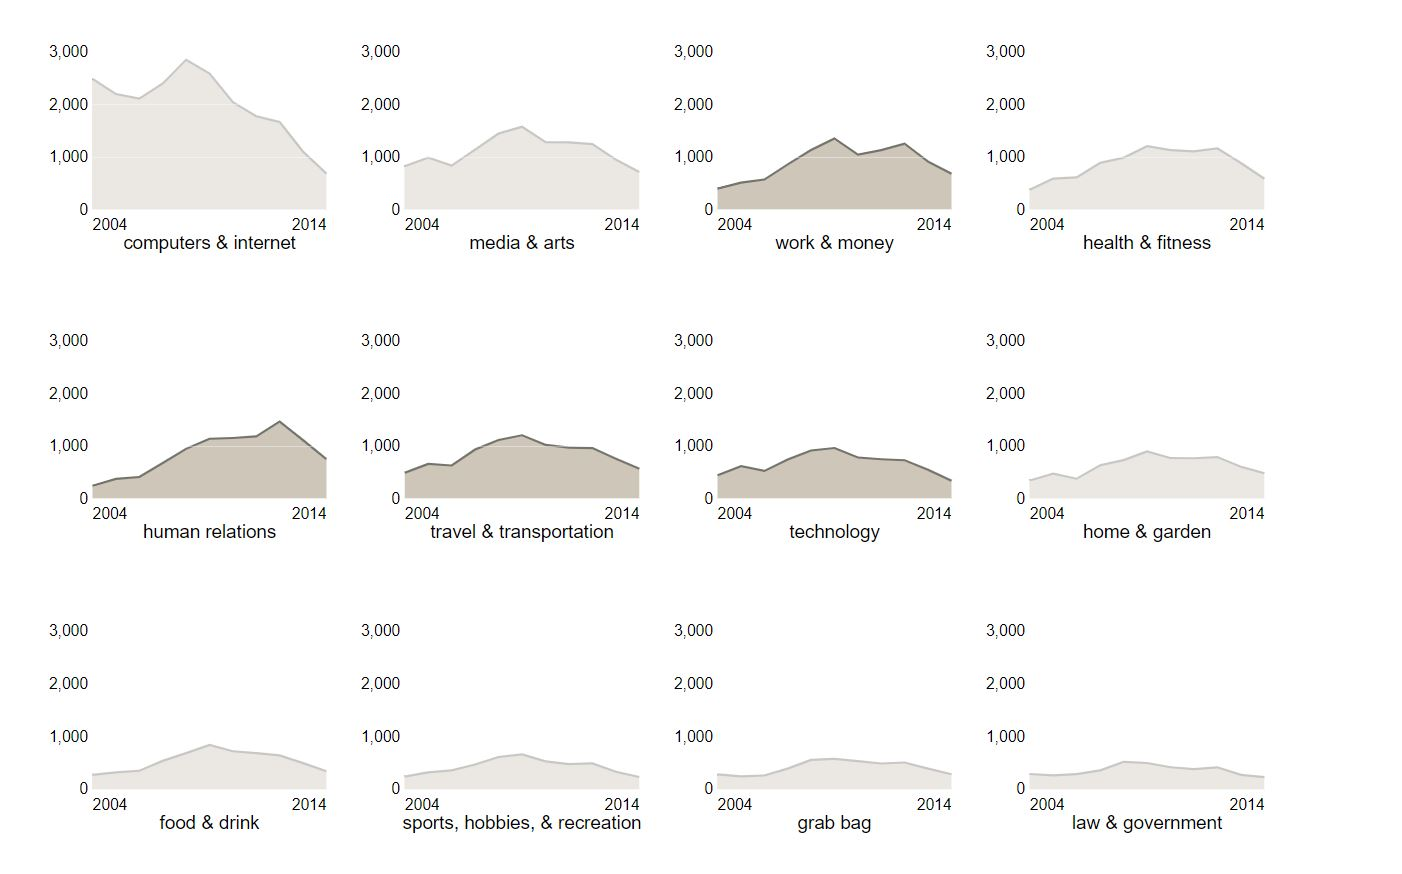
\includegraphics[width=0.95\linewidth]{images/ch_2_interaction_history.JPG}
  \captionof{figure}{Example of Hindsight\cite{feng2016hindsight} system that visualizes interaction history by making visited charts appear darker.}
  \label{fig:ch_2_interaction_history}
\end{figure}


Exploring genomic information at different resolutions can be problematic due to a dataset's volume, complexity, and due to limitations in the availability of visual space but these problems can be addressed through effective interaction techniques. However, relying on interaction mechanisms to navigate visual spaces can come with its own set of problems, one of which is memorability. Memorability is the degree to which users can retain information about the position of objects and markers in a visualization and revisit them. Revisitation is important in data exploration as it can help users retrace their steps and is part of the \textit{history} stage of the information seeking mantra presented by Schneiderman\cite{Shneiderman96theeyes}. However, revisitation can be affected by interaction techniques that require users to switch between graphical representations or zoom into a particular region and cause them to lose context of their previous position. Humans primarily rely on spatial cognition to remember the locations of objects in information workspace tasks but context-switching visual systems can disrupt this ability\cite{datamountain}. Similarly, interactive techniques such as fisheye views that work by distorting the original visualizations, can also impair spatial memory as shown by Skopik and Gutwin\cite{gutwin2003finding}. 


One of the methods by which this problem can be addressed is by storing the interaction history of the system and presenting it as a graphical abstraction either in the visual system itself or as an external panel. Interaction history can show the historical actions performed by a user and can also provide information on the actions performed so far that have led to the current state of the visual system. This interaction history can be provided indirectly through a history widget panel or by direct encoding into the visualization through the notion of \textit{readwear} or \textit{visitwear}. An example of  direct interaction history encoding in a visualization system is the visitwear mechanism developed by Skopik and Gutwin for fisheye views to highlight visited nodes. \textit{HindSight} is a similar direct encoding design framework that proved that users were able to visit more data points and recall novel insights by using their framework\cite{feng2016hindsight}. It encoded interaction history by making visited charts in a multi plot system appear darker, as shown in Figure \ref{fig:ch_2_interaction_history}, or relied on the existing visual encoding in line-charts and made visited lines slightly larger.

The second indirect encoding method for interaction history stems from research in visual analytics for supporting \textit{provenance} - which is the history of steps that led to a particular result in a data analysis workflow\cite{gotz2009characterizing,freire2008provenance}. The concept of provenance of visual history is centered around systems like the \textit{VisTrails} tool\cite{bavoil2005vistrails} that let users save visual outputs and revisit earlier states in the data analysis process. The notion of the earlier states termed as \textit{graphical histories} is explored further by Heer et al.\cite{heer2008graphical} in their graphical history interface for the Tableau visualization system.
In the context of genomic visualizations to the best of our knowledge direct encoding of interaction  history has not been explored but some recent synteny visualization tools like AccuSyn have offered partial support for revisitation through indirect encoding by letting users manually capture states of the system and revisit them through a history panel \cite{accusyn}.
\chapter{Data and Task Abstraction}

SynVisio was developed over multiple iterations as the necessary data and requirements were refined through continuous consultation with our genome research collaborators. To understand the design choices for visual encoding and interaction that we adopted in developing SynVisio, we need to first elaborate on the underlying data and task abstractions. We start with the data abstraction, where we explain the different characteristics of the syntenic data and how it is computed using synteny detection tools and further processed by our system. We then explore the different analysis tasks that can be performed on syntenic data, and finally, we discuss supplementary requirements that help researchers in using and interacting with SynVisio.

\section{Data}
This section starts with the description of the structure of a genome and its constituent elements and follows through with an explanation of how syntenic data is generated and represented.

\subsection{Genome Structure and Scales}
The genome of every organism is unique and can be defined as the complete set of DNA needed to build and maintain that organism. Structurally, genomes are broken down into smaller sections called chromosomes, where every chromosome is a long strand of DNA coiled up along with various proteins. Each chromosome is made up of several genes, which are the basic functional units of heredity and which code for a specific protein. Genes can then be further broken down into nucleotides which are the smallest building blocks of DNA. For analyzing genomic conservation, researchers also look at a collection of collinear genes that are called blocks. Thus the genome structure can be ordered into the following five levels from top to bottom in terms of genomic size : \textit{Genome\textrightarrow{Chromosome}\textrightarrow{Block} \textrightarrow{Gene}\textrightarrow{Nucleotide}}. However, to analyze large scale genomic conservation we only look at the first four levels. The structural data of a genome describing its constituent entities is provided in the form of a \textit{GFF(General Feature Format) File}. It contains the start and end position of every gene on a linear scale in a chromosome, the gene identifier, and the reference name of the parent chromosome in a three column tab-delimited format. A partial GFF file can be seen in Figure \ref{fig:ch_3_gff_file}.  Information on several genomes belonging to different species can be presented in the same file; each species is distinguished by the two-character key present in the reference name of the chromosome. The data in the GFF file is processed by SynVisio to get the genomic size (number of nucleotides) of the different genomes and their constituent chromosomes along with the size and position of all the genes within these chromosomes. This data gives us a precise structural map of every genome and its different sub-elements and so can be used to visualize a genome over multiple scales and levels.

\begin{figure}
  \centering
  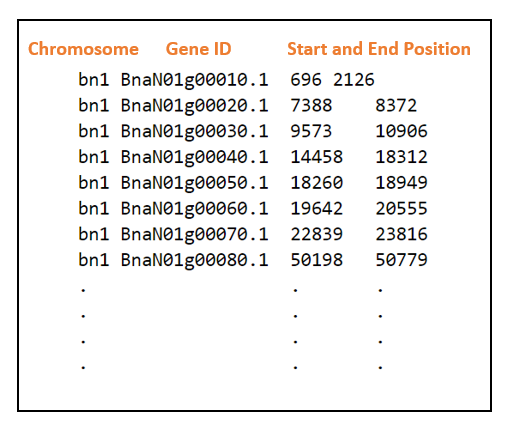
\includegraphics[width=.55\linewidth]{images/ch_3_gff_file.PNG}
  \captionof{figure}{Partial GFF file describing structure of a genome.}
  \label{fig:ch_3_gff_file}
\end{figure}


\begin{figure}
  \centering
  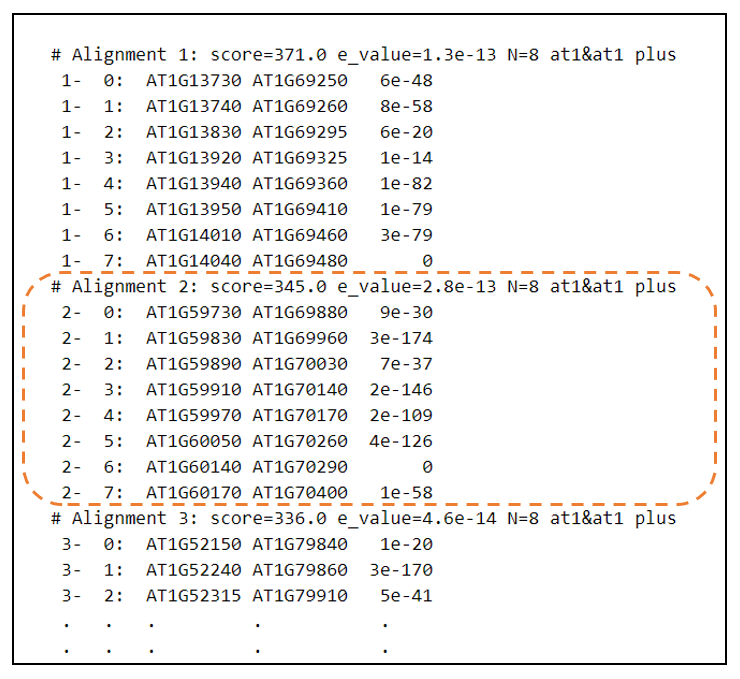
\includegraphics[width=.675\linewidth]{images/ch_3_coll_file.PNG}
  \captionof{figure}{Partial collinearity file with a single block highlighted.}
  \label{fig:ch_3_coll_file}
\end{figure}



\subsection{Conservation Data}
At the smallest level, conservation between two genes can be inferred by looking at sequence homology, which is the similarity between nucleotide sequences. Larger genomic conservation events can be studied by looking at blocks of such homologous genes and grouping them together based on their chromosomal positions to identify collinearity. To arrive at this data, we first identify all the homologous genes between two genomes using a local alignment tool such as BLAST (Basic Local Alignment Search Tool)\cite{blasttool}. Different synteny detection tools then construct collinear blocks of these homologous genes by either clustering neighbour matching gene pairs (ADHoRe, OrthoCluster) \cite{proost2011adhore,zeng2008orthocluster} or by constructing chains around an anchor gene (MCScanX)\cite{wang2012mcscanx}. These collinear blocks are referred to as syntenic blocks, and are the primary source of data for SynVisio and are provided as a collinearity file. A partial sample of a collinearity file can be seen in Figure \ref{fig:ch_3_coll_file}. Every block of collinear genes has a corresponding similarity score indicating the quality of match; an expect value (\textit{E-value}) indicating the probability that the match may have been due to chance; the count of genes; the names of the source and target chromosomes that the block of genes belong to; and the orientation of the block(forward or reverse). Finally, every block of data also consists of a list of the homologous gene pairs in that block and their statistical significance (\textit{E-value}). This data, combined with the information about the structure of the genome can be used to associate every region of a genome with its homologous regions in the other genome or within itself depending on the type of synteny under investigation.


\subsection{Auxiliary Track Data}
Since genomic data is represented as a collection of linear sequences, additional information can be provided in the form of tracks parallel to the original gene sequence structure. These tracks can contain information about genomic features such as gene density, copy number variations (CNVs), and single-nucleotide polymorphisms (SNPs). The data is provided to SynVisio in a BedGraph file format consisting of four tab-delimited values: chromosome identifier, chromosomal start position, chromosomal end position, and a data value. This information can be hierarchically grouped at the block or chromosome levels in the same way as genomic sequences and can be used to annotate the corresponding sequence structure. 

\begin{figure}
  \centering
  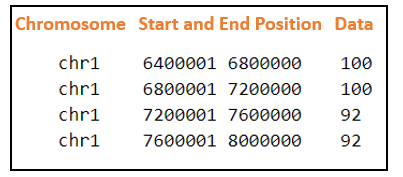
\includegraphics[width=.45\linewidth]{images/ch_3_track_file.PNG}
  \captionof{figure}{Sample track file.}
  \label{fig:ch_3_track_file}
\end{figure}

\section{Tasks}

In this section, we look at the different questions researchers have when analyzing genomic conservation. We then collate all the design requirements into a series of analysis tasks and group them based on the conservation relationship they address. Finally, we elaborate on some additional elements that improve the usability of the system and assist users in performing their analysis tasks.

\subsection{Requirement Gathering Phase}
To formulate our design requirements, we met with three groups of researchers working in different fields of biological research. The meetings were conducted over several iterations to refine our initial requirements. The sessions broadly revolved around understanding the basic tasks researchers perform when analyzing genomic conservation and looking at the shortcomings of the existing synteny analysis tools on the market. Although all three groups were primarily interested in analyzing synteny, their individual use cases varied, providing us with a diverse set of user scenarios.

Our first research group was involved in researching genomic conservation in the \textit{brassica} genus as it offers an ideal model to study polyploid evolution, which is responsible for genetic variations that are advantageous from an evolutionary perspective\cite{madlung2013polyploidy,liu2014brassica}. In particular they were interested in understanding genomic conservation within an allotetraploid species \textit{Brassica napus}(AACC), an important oilseed crop, and also in comparing it to the closely related diploid species \textit{Brassica rapa}(AA) and \textit{Brassica oleracea}(CC) that belong together in the classical triangle of U\cite{nagaharu1935genome}. The requirements from this research group were focused around having access to a system that could let them visualize the conserved relationship between the different diploid species and also within the chromosomes of a single allotetraploid (i.e. self-synteny). 

The second research team was interested in looking at genomic conservation between \textit{Lens culinaris} and \textit{Cicer arietinum} to improve various agronomic traits, as these are both widely grown legume crops. The requirements here were largely focused on cross synteny rather than self synteny. A unique trait of this particular dataset is that while \textit{C. arietinum} has a genome size of 740 Mbp, \textit{L. culinaris} has a genome size of 4 Gbp. This vast difference in the sizes of the two genomes makes visualizing synteny at the whole genome level extremely difficult and researchers must hence rely on comparing individual chromosomes of \textit{L. culinaris} one at a time or rely on a visualization that can have variable scales between the source and the target genomes.


The final research group works on sequencing wheat, and the researchers in this group were interested in understanding the genomic conservation between the three subgenomes of the hexaploid bread wheat genome. Researchers from this team wanted a system that could visualize synteny between three different genomes instead of a single source and target, while taking into consideration the extremely large size of the wheat genome. They were also interested in adopting a novel network-based visualization called a Hive Chart\cite{krzywinski2011hive}, which maps nodes onto radially distributed linear axes, for exploring multi-way genomic conservation.

\subsection{Visual Analysis Tasks}
Based on the underlying data and the requirements gathered from our research collaborators, we can group all analysis tasks performed in exploring genomic conservation into three basic groups according to the genomic scale at which they operate.

\smallskip
\noindent
\textbf{Genome Level}
\smallskip
\begin{enumerate}
\item [$Q_1$.] What is the level of conservation that exists between two or more sets of genomes?
\item [$Q_2$.] How does the density of conservation change across the genomes, and are there any gaps?
\item [$Q_3$.] How does the ordering of chromosomes based on conservation change between a given set of genomes or within a single genome? (possibility of detecting whole-genome duplication or genome reversal )
\item [$Q_4$.] If unmarked scaffolds exist, which regions of the target genome do they share similarity with?
\item[$Q_5$] Which chromosomes are sparsely or entirely unaligned, and how does the level of conservation change when these are ignored ?
\end{enumerate}

\smallskip
\noindent
\textbf{Chromosome Level}
\smallskip
\begin{enumerate}
\item [$Q_6$.]What is the level of conservation between a specific subset of chromosomes?
\item [$Q_7$.] What is the level of conservation between a single chromosome and an entire target genome or several other chromosomes (detecting unaligned regions within a chromosome)?
\item [$Q_8$.] 
How large are the collinear blocks relative to neighbouring chromosomes?
\item [$Q_9$.]What is the orientation of collinear blocks between two given chromosomes? (regular or inverted)
\end{enumerate}

\smallskip
\noindent
\textbf{Block Level}
\smallskip
\begin{enumerate}
\item [$Q_{10}$.]What is the level of conservation between the set of genes in a collinear block?
\item [$Q_{11}$.] What are the different genes contained in a block?
\item [$Q_{12}$.] What is the size of a gene relative to the size of the collinear block?
\item [$Q_{13}$.] Are there large gaps between genes in collinear blocks?
\item [$Q_{14}$.] Answer $Q_{10}$-$Q_{13}$ when a collinear block is reversed?
\end{enumerate}

There are also several other analysis tasks that researchers perform that go beyond the block level and down to the nucleotide level. However, these tasks are beyond the scope of this project; there are several other systems specifically designed to investigate collinearity at the nucleotide level, such as JBrowse \cite{skinner2009jbrowse}.


\subsection{Supplementary Design Requirements}
In addition to requirements raised by questions $Q_1$-$Q_{14}$, we also explore other design requirements that were raised during our discussions with our research collaborators. 

\textbf{Data Refinement} The underlying data that answers questions $Q_1$-$Q_9$ can be noisy due to incorrect parameter values used during synteny detection. This data can be filtered further based on several data attributes of the conserved blocks such as the similarity score, gene count, and expect value (\textit{E-value}). This requires an interactive feature in the visual design of the system that can assist researchers in extracting a subset of the original dataset based on a particular threshold of a specific data attribute. Another direction in which this requirement can be extended is having the ability to search for a specific gene in a dataset to look at all collinear blocks containing the gene.

\textbf{Data Enhancement} Analysis Tasks $Q_1$-$Q_9$ can be improved by providing a secondary data series that can contain additional information about the original sequences such as gene density and SNPs mentioned in sub section 3.1.3. This can also make it easy for researchers to identify patterns relative to known genomic markers.

\textbf{Data Exploration} Researchers need a system that offers multiple visual representations of the same information instead of relying on a single visualization, in order to explore the richness of the data shown by different data attributes such as size, location, proximity, and orientation of the conserved regions.

\textbf{Revisitation Support} The ability to simultaneously refine, enhance, and explore complex data visualizations during synteny analysis can often overload the spatial cognition of the user, causing them to lose track of their location in their workspace. This needs to be avoided and users need to be given a way to revisit the various steps in their synteny analysis pipeline when exploring a complex dataset.

\textbf{Web Access} In an increasingly connected world where research happens between a diverse set of collaborators spread across the globe, there is an increasing need for synteny analysis systems to be available as web applications. Researchers need the final system to be accessed through a website that can let them directly upload the results of synteny detection tools to visualize the required information.





\chapter{Visual Design}

Visualizing syntenic data is a multi-faceted problem as not only can the visual representation change based on the underlying biological question but also the resolution at which the information is being visualized. In designing a solution for this problem, the taxonomy of design space created by previous synteny visualizers like Mizbee \cite{Meyer2009} was adopted and further enhanced with our recommendations for representing synteny in multi-way comparisons. In designing SynVisio we used two primary forms of visual representations, a parallel plot, and a dot plot, and modified them to work across multiple data resolution levels. We also created hybrid plots based on our parallel plot design to represent synteny in multi-way comparisons. In this chapter, we first discuss the different forms of visual encoding used in our system. We follow this with a  description of the different layout strategies that were explored. Then we elaborate on the various interaction strategies we adopted based on the visual information seeking mantra framework and design of multiple coordinated views. Finally we end the chapter with a discussion on our iterative design process through 4 major development cycles.

\begin{figure}[h]
  \centering
  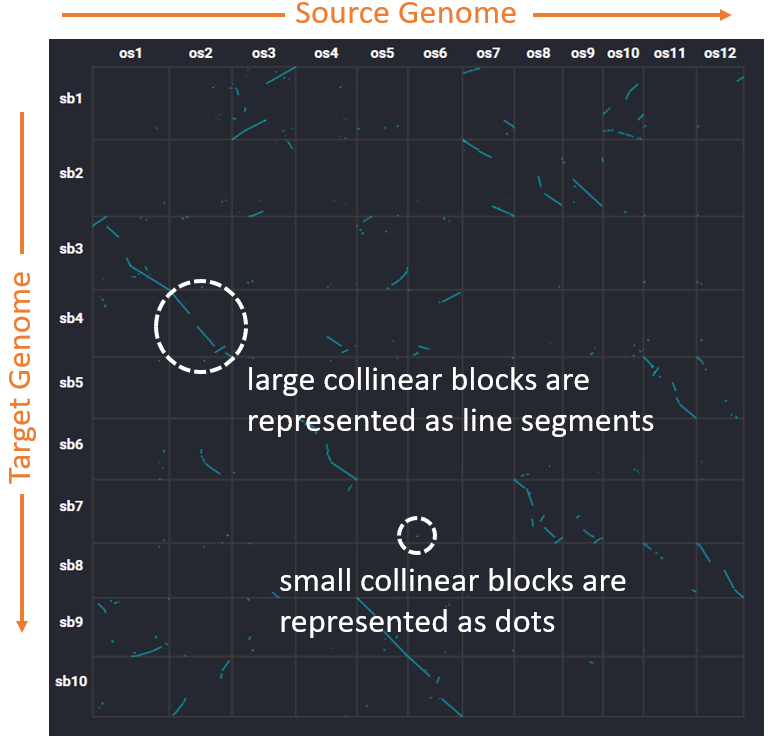
\includegraphics[width=.475\linewidth]{images/ch_4_dot_plot_a.PNG}
  \captionof{figure}{Dot plot showing whole genome synteny between Oriza sativa(rice) and Sorghum bicolor(corn) with grid-lines added for chromosomal boundaries.}
  \label{fig:ch_4_dot_plot_a}
\end{figure}


\section{Visual Encoding}

A common way to represent sequence alignment or similarity is to visualize it as a two-dimensional `dot plot' \cite{SONNHAMMER1995GC1,Cabanettes2018} through positional encoding. We adopted this strategy for our first visual representation by placing the source and target genomes along the \textit{x} and \textit{y} axes, respectively, and marking gene alignments with dots as shown in Figure \ref{fig:ch_4_dot_plot_a}. Grid-lines were then further added to the plot to indicate chromosomal boundaries.



This plot can also be adopted for other resolutions by changing the genomes along \textit{x,y} axes to either individual chromosomes or smaller gene blocks. Such matrix-based representations are very good at providing an overview of the dataset and can be used to highlight breaks, inversions, and duplications, as shown in Figure \ref{fig:ch_4_dot_plot_b}. However, being a relatively primitive visual representation dot plots are often found to be visually unappealing and complex to understand without the proper background context, making them unsuitable for a variety of exploration and communication tasks.


\begin{figure}
  \centering
  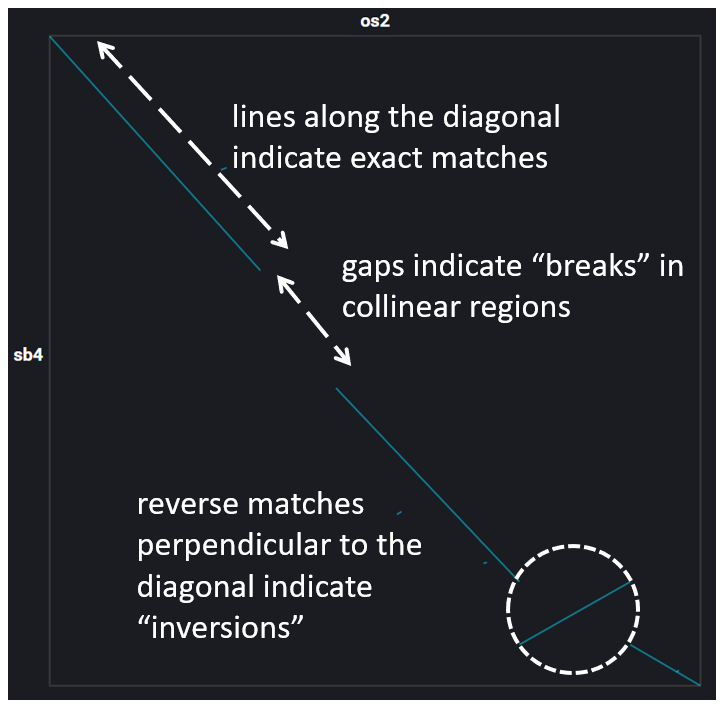
\includegraphics[width=.475\linewidth]{images/ch_4_dot_plot_b.PNG}
  \captionof{figure}{Dot plot showing breaks,inversions and duplication events between chromosome 2 and 4 of Oriza Sativa(rice) and Sorghum Bicolor(corn) respectively.}
  \label{fig:ch_4_dot_plot_b}
\end{figure}


For our other primary visual representation, we adopt a design that represents synteny through a combination of positional encoding for genomic distances and connected lines for similarity. In this approach, genomic sequences are stacked horizontally parallel to each other, and similar genes are connected through lines to indicate similarity. However, unlike dot plots that use the same visual encoding across all genomic sizes, for this visual representation, we adopt a different secondary encoding based on the resolution of the genomic sequences being visualized. 

\begin{figure}][ht]
  \centering
  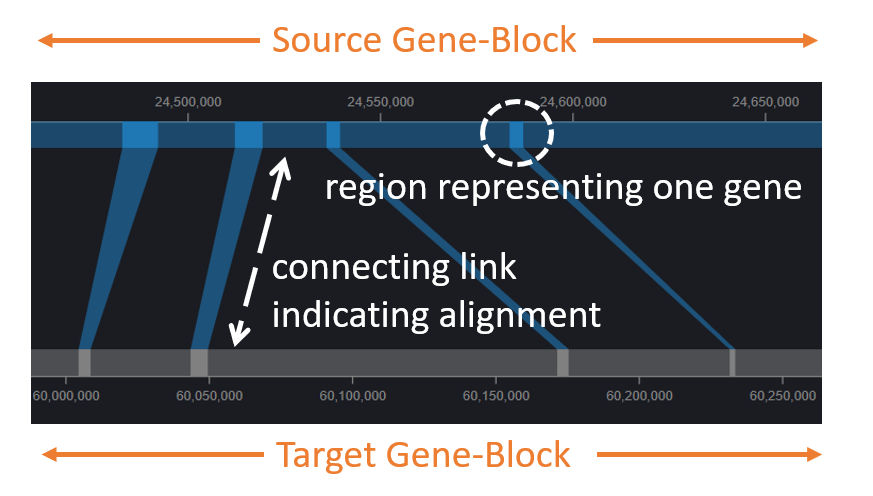
\includegraphics[width=.50\linewidth]{images/ch_4_link_plot.PNG}
  \captionof{figure}{Parallel Plot at the Gene-block Level}
  \label{fig:ch_4_link_plot}
\end{figure}


There are three basic levels in which synteny can be visualized starting from the gene block level, which is the smallest unit at which syntenic data is reported. A gene block is a collection of collinear genes in the source genome that are aligned to a group of collinear genes in the target genome. To encode conservation at this level, we use two gene blocks that are represented by line segments, and are stacked parallel to each other. Similar genes within the blocks are then connected with ribbons, as shown in figure \ref{fig:ch_4_link_plot}. The connecting ribbons are four sided polygons whose edge widths are dependent on the number of gene pairs in the collinear block at each edge. The source and target gene blocks are annotated with numeric tracks corresponding to their position in the chromosome and are coloured in distinct colours to distinguish them. The individual genes are represented as rectangles highlighted with a deeper shade of the base colour of the track for easier reference. 

At the next level, individual chromosomes are considered since a collection of gene blocks form a chromosome. Visualizing synteny at this level involves encoding information related to the location, size and orientation of conserved regions. To achieve this, chromosomes are stacked parallel to each other and their lengths are encoded to reflect their genomic size. So chromosomes with more base-pairs in them show up as longer line segments. Conserved regions in the chromosomes are then connected through ribbons from their positions on the chromosome to indicate similarity. This encodes both the location and the size of the conserved regions as the width of ribbons changes based on the genomic size of the linked gene blocks.


\begin{figure}[h]
  \centering
  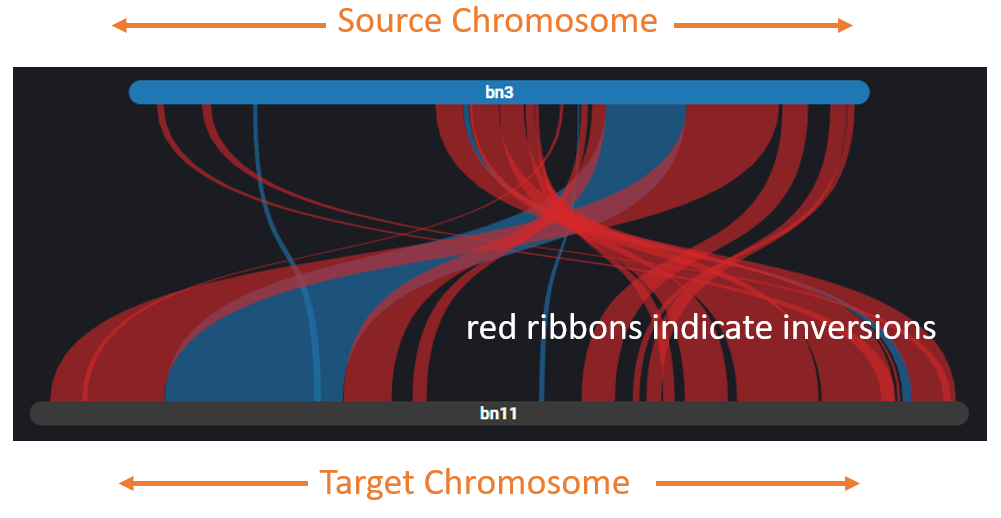
\includegraphics[width=.60\linewidth]{images/ch_4_link_plot_chromosome_a.PNG}
  \captionof{figure}{Link Plot at the Chromosome level where the blue coloured ribbons represent forward matches and the red coloured ribbons represent reverse matches(inversions).}
  \label{fig:ch_4_link_plot_chromosome_a}
\end{figure}


To encode the orientation of the gene block, secondary encoding in the form of colour is adopted to visually distinguish gene inversions, as shown in figure \ref{fig:ch_4_link_plot_chromosome_a}. So forward matches are coloured in blue, and reverse matches are coloured in red. Unlike the gene block level, at the chromosome level several bands can overlap and cross each other due to multiple gene translocation and inversions events and can cause visual clutter. To mitigate this problem, complex polygons are used instead of rectangular ribbons and are generated through \textbf{B}-spline curves\cite{ref851370272} with control points set to bundle the curves towards the centre\cite{zhou2013edge}. The control points are adjusted to be vertically in the middle of the parallel blocks to ensure that the original size of the ribbons remain undistorted at regions where they join the chromosome as they visually represent the size of the conserved region as shown in figure \ref{fig:ch_4_link_plot_chromosome_b}. 

\begin{figure}
  \centering
  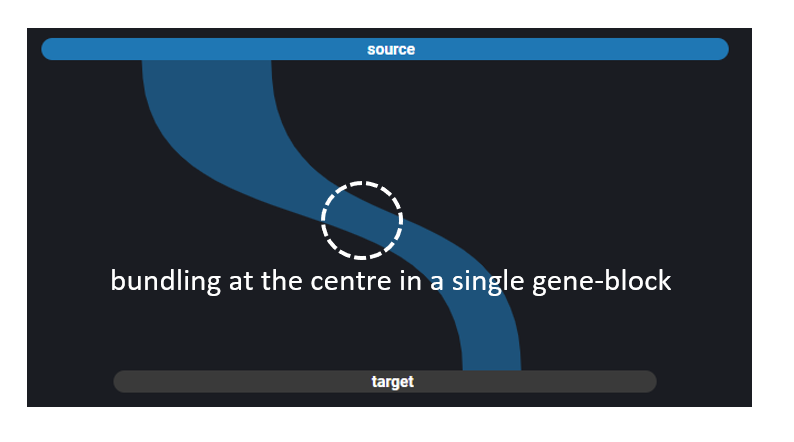
\includegraphics[width=.50\linewidth]{images/ch_4_link_plot_chromosome_b.PNG}
  \captionof{figure}{Ribbon bundling to reduce visual clutter with the control points set towards the centre indicated in a single gene-block.}
  \label{fig:ch_4_link_plot_chromosome_b}
\end{figure}


Finally, at the whole genome level where synteny is observed between several chromosomes at once, smaller details such as inversions have lower priority, and so the secondary encoding in the form of colour is used to distinguish different chromosomes instead of the orientation of the syntenic region. A layout similar to the parallel stacking at chromosome level is adopted, however, instead of having a single connected unit for the entire genome, chromosomes are separated from each other with gaps serving to indicate the start and end of each chromosome. Chromosomes in the source layer are assigned a unique colour, while chromosomes in the target layer are assigned through an alternating gray colouring scheme. Ribbons are then linked between conserved regions to represent syntenic gene-blocks and are assigned a colour based on their source chromosome.This form of encoding location information about the source in the connection through colour has been used earlier in other synteny visualisations systems and has been proved effective \cite{Meyer2009}. We adopt the aforementioned bundling strategy of using \textbf{B}-spline curves\cite{ref851370272} to improve visual clarity but set the control points independently for every chromosome to group all the gene blocks emerging from each chromosome into a single bundle.


\begin{figure}[ht]
  \centering
  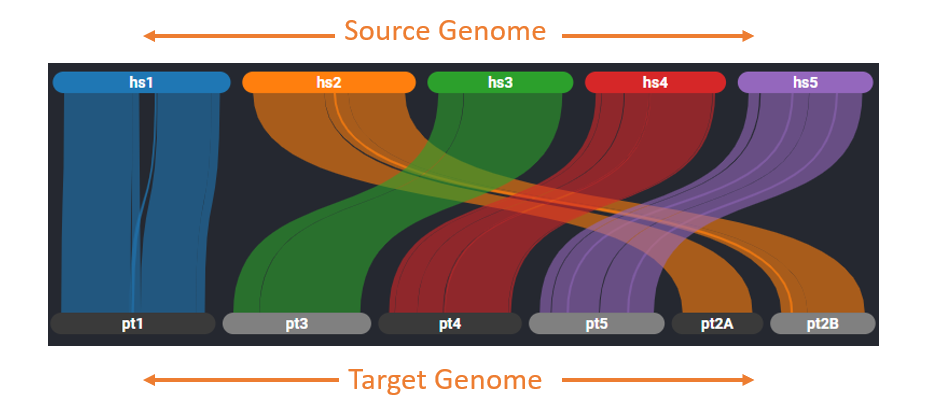
\includegraphics[width=.75\linewidth]{images/ch_4_genome_level.PNG}
  \captionof{figure}{Visual encoding at the chromosome level with connecting ribbons coloured based on the source chromosome they are linked from.}
  \label{fig:ch_4_genome_level}
\end{figure}



\section{Layout Strategies}

A common strategy that is used among all the three parallel stacked representations is the vertical separation between the source and the target to visually distinguish the two regions. This is easy to implement at the gene-block level, and the chromosome level as the source and target regions are single continuous entities but requires minor adaptations at the genome level. The genome is a combination of several chromosomes, so each chromosome had to be individually distinguishable while still being represented as a part of the whole source group and different from the target group. To achieve this grouping, we use the visual law of proximity from Gestalt principles \cite{wertheimer1923untersuchungen} which states that proximity can override other visual similarities (shape, size, colour) to differentiate a group of objects. and represent each chromosome as a pill-shaped region and then lay them out end to end horizontally with small gaps between them. The gaps between the chromosomes achieve the task of making the chromosomes look distinct and also being smaller than vertical gaps between the two genomes, clustering the source and the target regions into two separate groups visually.

\begin{figure}
  \centering
  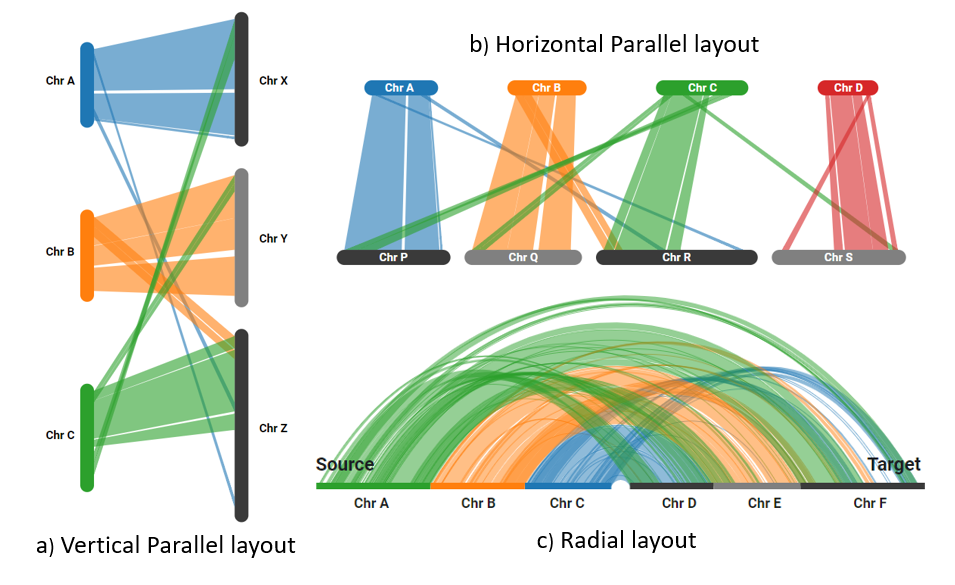
\includegraphics[width=.85\linewidth]{images/ch_4_layout.PNG}
  \captionof{figure}{Different layout strategies at the genome level with conservation being encoded as connections.}
  \label{fig:ch_4_layout}
\end{figure}


In arriving at the optimal layout strategy, we looked at several different alternative ways of arranging the chromosomes. In the popular synteny browser MizBee\cite{Meyer2009} the authors provide a taxonomy of the different synteny layouts and broadly classify them into two categories: contiguous and discrete. In the former, the chromosomes are presented adjacent to each other either in a linear or a circular layout, and in the later, chromosomes are treated as distinct elements, and presented either in segregated groups or interleaved with each other. In our design we go for the contiguous scheme, but we omit the circular layout as it has already been explored in AccuSyn\cite{accusyn}  and instead look at possible linear layout strategies where conservation is encoded through connections as shown in figure \ref{fig:ch_4_layout}.In the vertical(a) and horizontal layouts(b) the underlying approach is similar except for the orientation of the two parallel layers. However the number of chromosomes in a genome can be numerous as in the case of humans who have 23 and can cause the vertical layout to be quite long. This makes it sub-optimal for most standard screen aspect ratios. Therefore of the two, the horizontal parallel layout is the preferred mode of encoding synteny. A common advantage of these two layouts is that they can be stacked in multiple layers such that chromosomes at every level are linked to both chromosomes above them and also the chromosomes below them, as shown in the layout (a) in figure \ref{fig:ch_4_layout_multi}. This stacked layout strategy is used to represent synteny in the form of a tree view chart and can be particularly useful in scenarios where conserved regions need to be traced across several evolutionary levels.

\begin{figure}[ht]
  \centering
  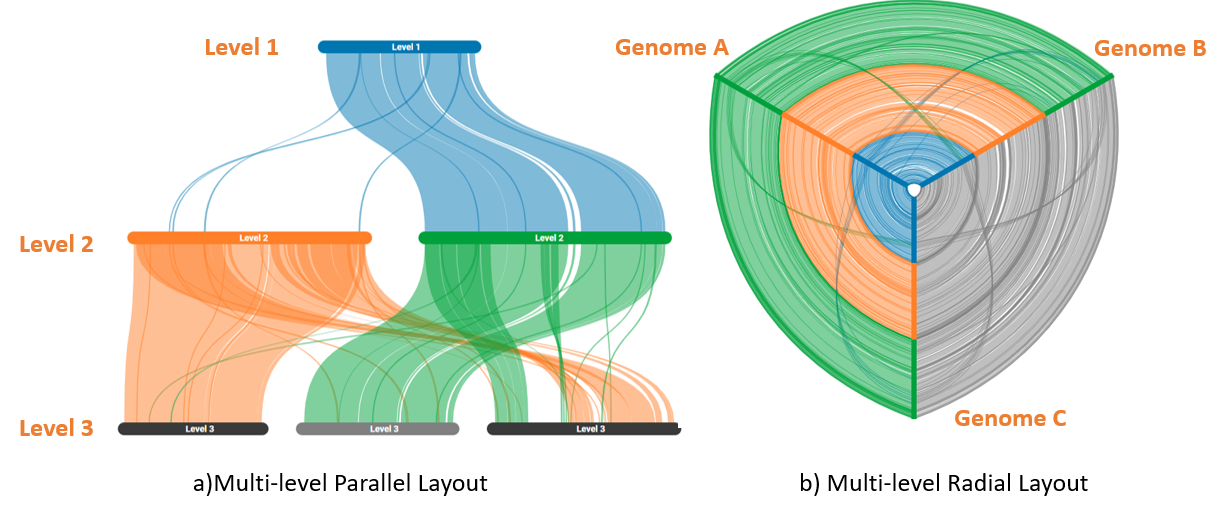
\includegraphics[width=.95\linewidth]{images/ch_4_layout_multi.PNG}
  \captionof{figure}{Multi-level layouts.}
  \label{fig:ch_4_layout_multi}
\end{figure}

The bi-directional linking strategy is however, unavailable in the parallel layout scheme in pairwise comparisons scenarios but can be utilized by moving the two layers adjacent to each other, as shown by the layout(c) in Figure \ref{fig:ch_4_layout}. In this layout,  the chromosomes are in the same level thus making it possible for conserved regions to be linked in two directions either from the top or from down below. This allows us to include an additional layer of encoding. For example, if we had to represent the orientation of the conserved regions, we could link all forward matches through connections from the top, and all reverse matches through links from the bottom. The disadvantage of this layout is the high number of crossing between the connections. This can be made worse in scenarios where there is a high degree of collinearity between the two genomes due to the ordering of the chromosomes as every connection between the first chromosome in the source and the first chromosome in the target is crossed by all other connections emerging from the rest of the chromosomes in the source. An alternative approach to solve this problem includes reversing the layout of one of the layers or arranging the chromosomes in a radially outwards fashion in both the layers. This layout can also be extended to express synteny in multiple levels by merely increasing the number of radial layers such that each layer is connected to both the layer on its right and the layer on its left, as shown in the layout (b) in Figure \ref{fig:ch_4_layout_multi}.



Irrespective of the ordering or the layout of the chromosomes, they all have unique positions in a visual representation. This prevents them from being occluded by other items in that representation. This however is not the case for  visual encoding of conservation through lines or ribbons that can overlap significantly in some instances. The Z-axis position of the ribbons decides which ribbons occlude others and is dependent on the rendering order of the ribbons. To address this problem, we sort the conserved genes in every chromosome based on their gene count. This places smaller gene blocks at the end of the list ensuring that these blocks are rendered last, making them appear higher on the Z-axis and thus above the bigger blocks. To further solve this problem, connected ribbons are rendered with 75\% transparency, which ensures that even if ribbons end up overlaying other connected ribbons, they are still visible on the screen.

\section{Visual and Interaction Design}

Having discussed the different ways in which syntenic data can be encoded, we can summarise that the usefulness of a particular representation depends on the syntenic relationship under investigation. This has created a need for an adaptive system that can be used under a wide range of scenarios spanning investigation of micro synteny all the way up to high-level genome duplication events. Syntenic data also goes beyond the basic location, size and orientation of the conserved regions and includes additional information such as the match score and the E (expect)value, which indicates the level of similarity and the probability of a match occurring by chance respectively. This inherent complexity in the dataset means that exploring it becomes challenging as the volume of the data increases. Thus in designing our synteny exploration interface, we build on the framework of visual information seeking mantra \cite{Shneiderman96theeyes}. Our design framework breaks down synteny analysis broadly into the following tasks: overview, filter, zoom, details-on-demand, history, and extract.

We present information in a top-down tiered approach in three distinct scales starting with the whole genome followed by stepping down into an individual chromosome and finally ending on the gene block level. Users are giving the ability to start their investigation of the data at any particular level and pick either a dot plot, or a parallel plot, or a combination of both. Users are then given the option to interact with the visualizations in real-time to either filter the chart to look at conserved regions in a particular chromosome or drill down into the dataset all the way down to an individual gene in a conserved region as shown in figure \ref{fig:ch_4_exploration_through_interaction}. Additional details about the syntenic blocks are available on-demand through hover based mouse interactions either with the ribbons or the dots based on the type of representation.

\begin{figure}[h]
  \centering
  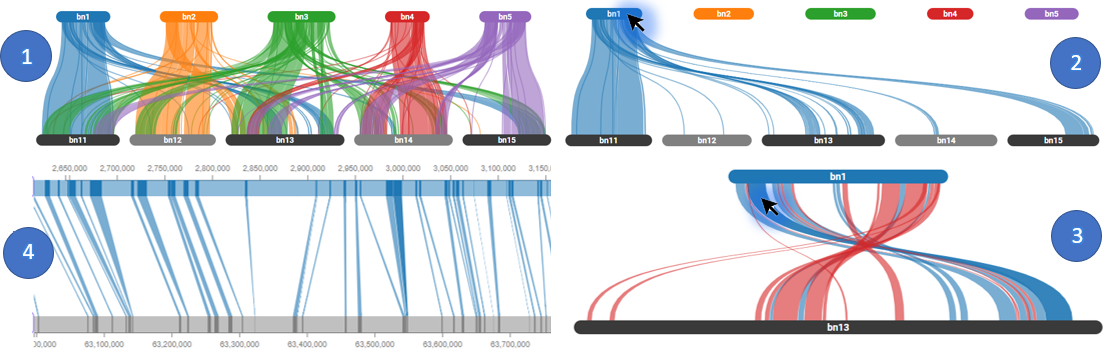
\includegraphics[width=1\linewidth]{images/ch_4_exploration_through_interaction.PNG}
  \captionof{figure}{User interactions in exploring conserved regions in a top down approach through 4 steps pictured in clockwise fashion.}
  \label{fig:ch_4_exploration_through_interaction}
\end{figure}


Our design also incorporates a dashboard for exploration where instead of relying on a single visualization, information about conservation at every level is presented through coordinated multiple views. This is built on the underlying premise that users have a better understanding of their data if they interact with the given information and view it through different representations\cite{Roberts}. In our design of multiple distinct views that support the investigation of a single entity, we followed the design guidelines set by earlier research into multiple coordinated views in information visualization systems\cite{WangBaldonado}. We present the following three distinct views, each highlighting a unique facet of the dataset : parallel plot, dot plot and a simple scatter plot that acts as a filter toggle. The parallel plot offers position and location information about the conserved regions at a glance while the dot matrix plot can easily highlight reversals and deletions within the conserved regions. Both the views are linked to each other to ensure that users don't lose context of their interaction. This is done by mirroring all actions between the two views. The final scatter plot is used to present the measure of similarity of the conserved regions and has a slider built into it that can be used to filter conserved regions based on their match score or E value. The filter works synchronously with the other two views and as the user moves the slider, the conserved regions are filtered in real time in the other two views. Finally, in keeping with the visual information seeking mantra framework, user interactions are recorded with users having the ability to store all their interactions in arriving at a particular analysis point as a visual stamp that can be revisited or reset back to in-case of further analysis.

\section{Iterative Development Process}
By following the guidelines of a standard design study methodology\cite{5290695}, our system design occurred iteratively over four main development cycles. At every stage, we presented our system to a panel composed of genome researchers and information visualization experts to gather feedback and look at possible avenues of improvement. After the initial requirement gathering phase we sketched a prototype of a linear parallel plot and a dot plot both visualizing conserved regions at the genome level. For our first development cycle, we used basic colours for distinguishing different chromosomes and encoded every collinear gene as a connecting link in the parallel plot and as a single point in the dot plot, as shown in figure \ref{fig:ch_4_first_iteration}. Although this approach helped in highlighting large scale patterns in genomic conservation, encoding every single gene meant that there was significant noise in the visualization that made it difficult to see the smaller conserved regions. Feedback was also directed at the choice of colour and and the layout of the lines in the parallel plot that caused them to visually occlude the lines right below them.

\begin{figure}
  \centering
  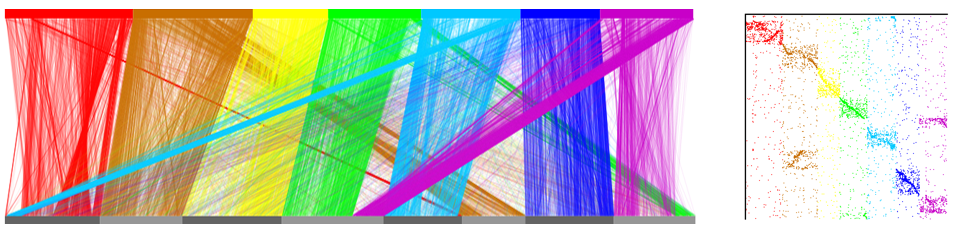
\includegraphics[width=1\linewidth]{images/ch_4_first_iteration.PNG}
  \captionof{figure}{Visual representations after the first development cycle consisting of a parallel plot(left) and a dot plot(right).}
  \label{fig:ch_4_first_iteration}
\end{figure}

\begin{figure}[h]
  \centering
  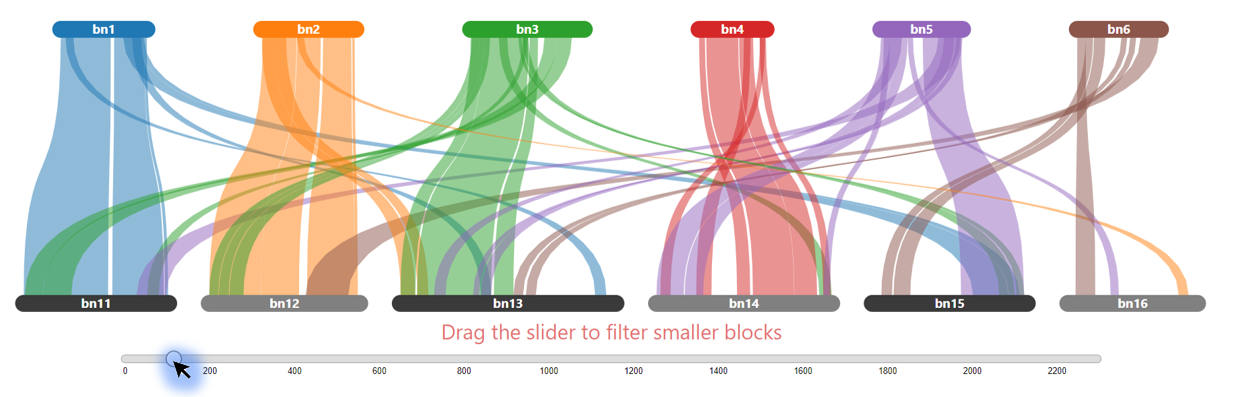
\includegraphics[width=0.85\linewidth]{images/ch_4_base_viewer.PNG}
  \captionof{figure}{Design after the second development cycle with a slider filter.}
  \label{fig:ch_4_base_viewer}
\end{figure}


For our second development cycle, we adopted two major changes: we broke down the syntenic data into three levels and limited top level visualizations to just representing collinear gene blocks instead of their constituent genes and, we added interaction features that let users select the chromosomes they wanted to observe instead of looking at the entire genome. Although grouping collinear genes into larger blocks helped reduce visual occlusion significantly, this problem was further addressed by an updated colour palette and converting connecting ribbons into curved B-spline curves instead of straight rectangular curves. Since dot plots are based on positional encoding we removed colours to identify chromosomes in the dot plots and instead relied on grid lines to act as chromosomal boundaries. New levels at the chromosome and the gene-block level were also added to visualize conservation at smaller scales. Finally, a simple slider interface was added to filter conserved blocks based on their gene count. Feedback at this level was largely directed towards the filter feature which despite being helpful was counter-intuitive to synteny exploration as the relevance of conserved regions is based on a combination of the level of similarity , the probability of the match occurring by chance and its constituent genes and not just the gene count. This is because filtering conserved regions is highly dependent on the subject under exploration and hence it needs to be contextually adaptive.


Development in our third iteration was structured around building a system that could be adapted for use in a wide range of scenarios. We developed a composite dashboard with coordinated views and a context-aware filter to help users in making a better-informed decision when they are filtering syntenic blocks. To improve usability, we also added multi-level comparison charts such as hive plots and stacked parallel plots to represent synteny beyond simple pairwise scenarios. For our fourth and final development iteration, we added features that were designed to improve user engagement with our interface, such as gene search and addition of secondary visual encoding in the form of heat-map or histogram tracks to the chart. Visual encoding for the gene search feature was primarily done through colour and vertical positioning. A gene block that contained the gene being searched for was coloured in white and brought to the front above the other gene blocks in terms of on-screen rendering in order to highlight it.
\chapter{SynVisio}

Our most significant contribution in this research was the development of SynVisio, an online platform to explore syteny by mapping syntenic blocks that are highly conserved and long enough to be significant between a given pair of genomes or within a single genome. In this chapter, we first discuss the different modes SynVisio offers for synteny analysis and how each one operates. We then explore the various features SynVisio provides to enhance user experience with the tool. Finally, we discuss the software implementation of the tool and then elaborate on the choices made in the web architecture of the system.

\section{System Overview}
SynVisio is a multi scale genome browser that can be accessed through the web to explore genomic conservation. It lets researchers upload output files of a synteny detection system of their choice and generates visualizations on-demand from the information in these files. It offers two analysis modes: primary analysis mode and a multi genome analysis mode. In the first mode, users can compare genomes two at a time through a dashboard where synteny is visualized as both a dot plot and a linked parallel plot. The charts are accompanied by a filter panel where the conserved genomic blocks can be filtered based on features such as the degree of similarity. In the second mode, researchers can compare several genomes at a time through multi-level representations such as hive plots and stacked parallel plots. To aid researchers in their visual exploration of synteny, SynVisio lets them annotate the generated charts with additional tracks in the form of histograms, heat-maps and other basic plots. Additional features are also provided, such as a gene search panel to look for specific genes by gene ID and the ability to export generated charts for publication.


\section{Analysis Mode}
Gene sequences can be compared in different ways, depending on the underlying biological question. This means syteny analysis can vary from visualizing simple pairwise matches between two genomes to performing  multi-way comparisons across several genomes at once. The availability of datasets and their inherent quality also plays into the kind of analysis that can be done. Whole-genome alignment, for example, is usually done pairwise as looking for matches can be faster when the subset of available matches is low. Additionally, in the context of synteny detection, which is anchor-based (centered around genes), identifying common markers between multiple genomes is difficult\cite{wang2012mcscanx}. However when the data is available, multi-way comparisons can offer better insights and tackle more significant questions like pan-genome synteny. Thus SynVisio offers both a primary analysis mode for simple pairwise comparisons within a genome or between two genomes and a multi genome analysis mode for analysing conservation across several genomes, depending on the researcher's choice and the availability of data.

\subsection{Primary Analysis Mode}
This is the default mode in which SynVisio operates and is meant for exploratory tasks as it presents the collinearity between a selected set of chromosomes in two different visual representations and lets users filter the collinear blocks in real time. Although our system operates as a dashboard with multiple representations in coordinated views, we also offer users the ability to look only at one particular representation through the configuration page. This is meant to make our system unopinionated in the choice of visual representation and let users decide on how they want their data to be visualized. 

\begin{figure}
  \centering
  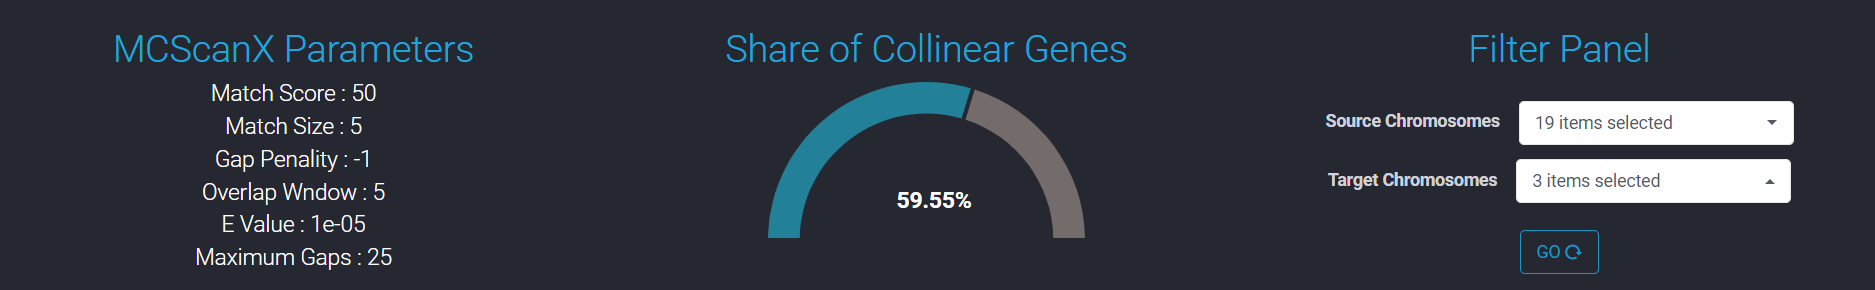
\includegraphics[width=1\linewidth]{images/ch_5_baseparameters.PNG}
  \captionof{figure}{Synteny detection parameters and level of collinearity presented along with toggles to select source and target chromosomes.}
  \label{fig:ch_5_baseparameters}
\end{figure}


The first step involved in using the dashboard is providing an input dataset; for this, users can either upload their own datasets or use existing sample files. We have already processed several datasets depicting genome conservation on a wide range of species. These are available on the homepage of our application and are updated on a regular basis. Some of the examples include self synteny in \textit{Brassica napus} (canola), cross synteny between \textit{Oriza sativa} (rice) and \textit{Sorghum bicolor} (broom-corn) and cross synteny between \textit{Arabidopsis thaliana} (thale cress) and \textit{Vitis vinifera} (grapevine). After the initial data uploading and processing stage is complete, basic information about the parameters used in the synteny detection process is presented along with the overall collinearity present in the files accompanied with toggles to select the source and target chromosomes as shown in Figure \ref{fig:ch_5_baseparameters}. If outputs of synteny detection systems other than MCScanX are uploaded, the parameters tab and the percentage share of collinear genes chart are replaced with a textual panel describing the features of the data on file including a list of all unique chromosomes and the total number of collinear blocks. The list of chromosomes is ordered alpha-numerically to divide the different species into distinct groups and make it easier to pick chromosomes sequentially. Additional buttons are also provided to either \textit{Select All} or \textit{Clear All} options in both the drop-down lists intended for choosing chromosomes. The dashboard operates in three views based on the level of genomic resolution, and each of these stages are described individually below.

\begin{figure}
  \centering
  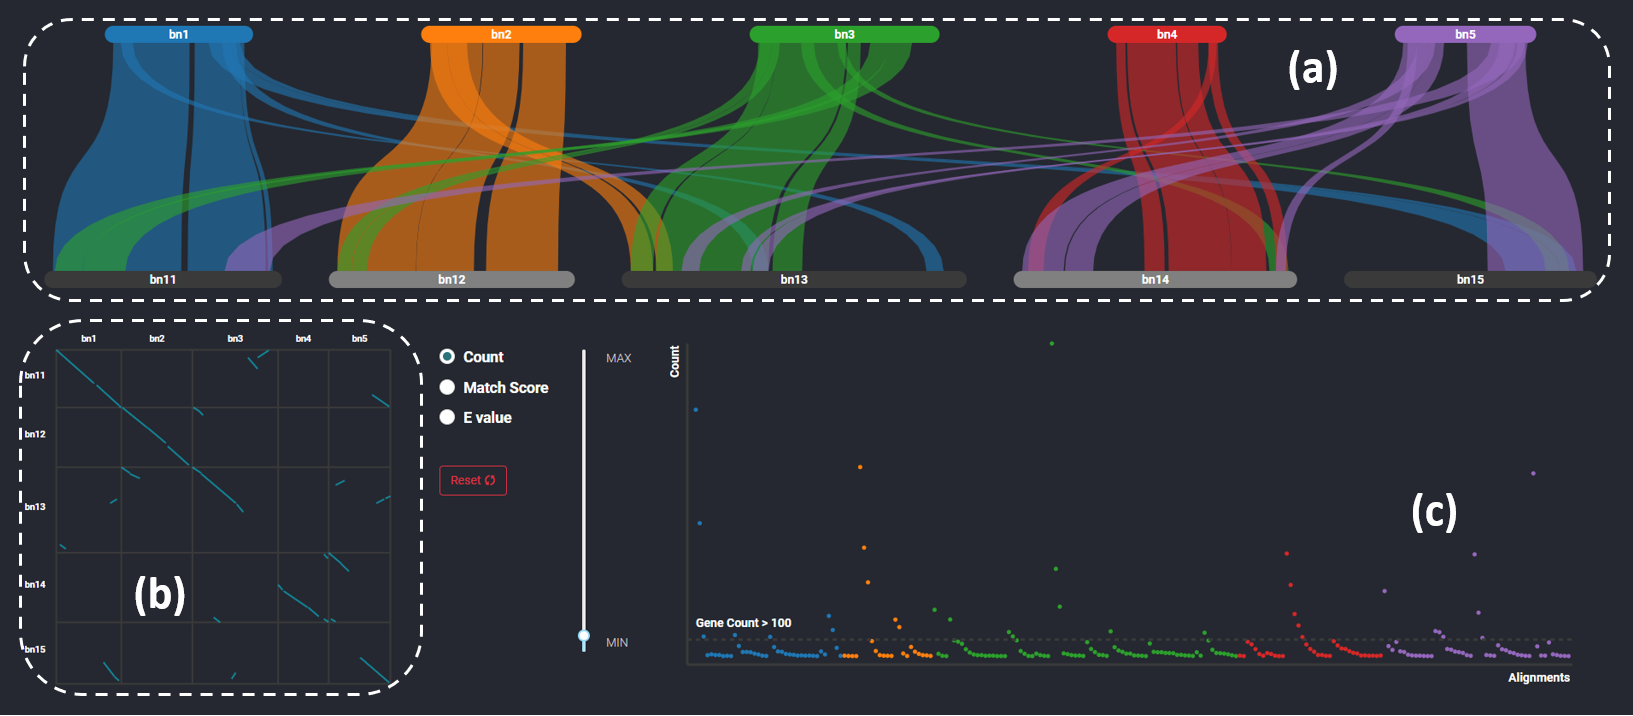
\includegraphics[width=1\linewidth]{images/ch_1_dashboard.PNG}
  \captionof{figure}{Genome View in the primary analysis mode with the following components: \textbf{a)} Parallel Link Plot \textbf{b)} Dot plot and \textbf{c)} Filter panel}
  \label{fig:ch_4_dashboard}
\end{figure} 

\textit{Genome View:}
This view is chosen by default when a user selects more than one chromosome in the source or target selection drop-down and is intended for observing large scale patterns at the genome level.
The first visualization presented at the top is a parallel link plot where syntenic collinear blocks are connected by coloured ribbons, as shown in Figure \ref{fig:ch_4_dashboard}. The source chromosomes are laid out on the top and the target chromosomes are spread out at the bottom. The size of the chromosomes are calculated based on the genomic sizes of the chromosomes and the available screen width to ensure that the visualizations are accurate across different screen sizes. Chromosomes in the source layer are coloured using a chromatic 10 point colour scale derived from ColorBrewer\cite{colorbrewer} and are set to repeat after every 10 chromosomes as humans cannot perceive differences beyond a dozen colours\cite{ware2012information}.The connecting ribbons represent collinear blocks with the colour of a ribbon representing its source chromosome. These ribbons can have varying widths at either end due to the size of the collinear block they represent. Although collinear blocks have the same gene count at either side, the width of the block in terms of base pairs can be quite different at either side due to variable gap sizes between individual genes. This scaled representation of connected ribbons can also mean that certain ribbons can end up being smaller than a single pixel in width due to their small genomic size. Therefore, we clamp our scale at the lower end to 2 pixels to ensure that extremely small ribbons are still visible.


\begin{figure}
  \centering
  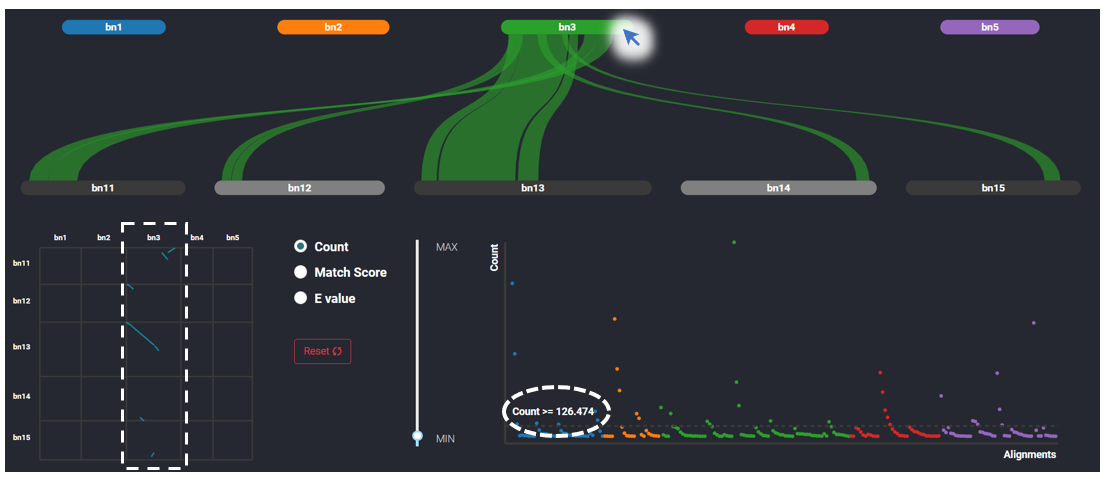
\includegraphics[width=1\linewidth]{images/ch_5_genome_view_2.PNG}
  \captionof{figure}{Genome View in the primary analysis mode with \textit{Chromosome 3} selected demonstrating the coordinated action being replicated in the Dot plot and the filter panel active with a target gene count set using the slider. } 
  \label{fig:ch_5_genome_view_2}
\end{figure} 


While the parallel link chart is designed to take half of the available vertical space on a standard 1080p screen, the other half is made up of a dot plot and an adaptive filter panel consisting of a scatter plot. The dot plot, as explained in the visual design chapter, uses positional encoding and represents collinear blocks as either dots or lines in a 2-dimensional matrix. To ensure that small collinear blocks are still represented on the screen, we limit them to single pixel wide dots on the chart while larger conserved blocks are encoded as lines. The dot plot works in a coordinated manner with the parallel link plot, and so any user action such as selecting a single source chromosome to highlight all conserved regions present in it, is also reflected in the other plot, as shown in figure \ref{fig:ch_5_genome_view_2}. Since the dot plot is always meant to be square, it has a fixed aspect ratio, and thus the filter panel expands to fill the remaining horizontal space. It provides filtering through three parameters: Gene count, Match Score, and E(expect) value. It is set to filter using gene count by default but can be changed using the radio buttons provided to the left. To offer users context into the parameter being filtered, its values across all the collinear gene blocks are visualized as a simple scatterplot. Every collinear gene block is represented by a single dot irrespective of its size and is colour coded to correspond to the source chromosomes in the parallel plot. The scale of the scatter plot is adaptive and automatically changes based on the parameter in question. Gene count and Match Score correspond to the number of genes in a collinear block and the alignment score assigned to that block, respectively, and are represented in a linear scale. E-value or expect value is the measure of the probability that a match has occurred by chance, and owing to the wide range in which this value can be reported it is represented in a logarithmic scale. Researchers can use the slider to control the visibility of collinear blocks they see in the other two views. The position of the slider on the chart is represented with a dashed line that is annotated with the value at which the charts are currently being filtered as shown in figure \ref{fig:ch_5_genome_view_2}.


\begin{figure}[ht]
  \centering
  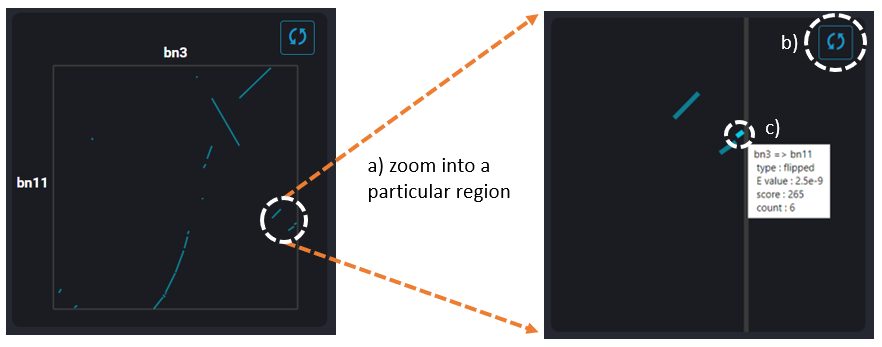
\includegraphics[width=.95\linewidth]{images/ch_5_chromosome_view.PNG}
  \captionof{figure}{Dot plot in the Chromosome View showing the ability to zoom into a particular region of interest (a), reset the zoom to the original state (b) and view additional information about a conserved block (c).} 
  \label{fig:ch_5_chromosome_view}
\end{figure} 

\textit{Chromosome View:} This view can be triggered in two ways, either by selecting a single source and a target chromosome using the drop-down selectors, or by clicking on a source and a target chromosome in the genome view. This acts as the logical second stage in exploring a genome where researchers can focus on a particular pair of chromosomes. At this stage, the layout of the visual representations remains the same however the visual encoding of colours to identify chromosomes is replaced with the orientation of the conserved regions with regular conserved regions represented as blue ribbons and inverted conserved regions represented in red. The adaptive filter panel also functions in the same way as in the genome view, but the dots in the scatter plot are not colour coded anymore to represent their chromosomal source. In this stage users are allowed to explore small scale patterns in conservation and thus have the ability to zoom into a particular part of the chart using mouse-based interactions, as shown in figure \ref{fig:ch_5_chromosome_view}. This feature is available to both the parallel plot and the dot plot, and the charts are provided with a reset button to readjust the scale of the charts to their original state. Finally, hovering the mouse over a conserved region in either plot will let users see additional information about that gene-block in an on-screen tool-tip.



\begin{figure}[h]
  \centering
  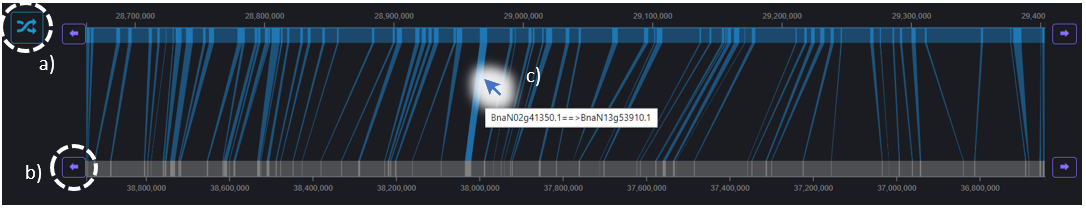
\includegraphics[width=1\linewidth]{images/ch_5_block_view.PNG}
  \captionof{figure}{Visualization in the Gene-Block View: a) Toggle button to flip the target gene block when exploring reverse matched gene blocks. b) Buttons to move the tracks horizontally along any one direction. c) On-screen tool-tip invoked by a mouse hover showing the source and target \textit{gene IDs} for a particular gene link.} 
  \label{fig:ch_5_block_view}
\end{figure} 

\textit{Gene-Block View:} This is the final view in the exploratory dashboard and can be accessed from the chromosome view by double-clicking on a particular gene block in either of the two plots that are available at that level. It offers an in-depth view of each of the constituent genes in a collinear gene block and only has a single parallel plot representation. Every connected link represents a single gene and the size of the link is based on the number of base pairs in that gene. This plot can be zoomed in just like the plots in the chromosome view, however, the zoom is applied to the horizontal scale, which means after zooming in at a point, users can then pan the chart either to the left or right look at adjacent genes. Users can zoom in to a large cluster of genes to look at every single gene pair and get their \textit{gene IDs} by hovering over a connected link. The horizontal zoom however, can cause distortion when linked genes are far apart, causing them to stretch when zoomed in. To address this issue, we provided the tracks with two buttons on either side of both the source and target tracks. These can be used to shift the scale in the required direction to ensure that the gene pairs under investigation are not distorted and instead correctly lined up. Another common issue that can occur in this view is the visual occlusion problem due to a high number of crossing in an inverted gene block. Gene pairs in an inverted gene block are linked across the opposite ends of the gene block and so any zooming into the gene block at this stage would cause the genes to stretch further apart. To address this issue, we provide a toggle button next to the chart whenever a gene block is identified to be a reverse matched conserved region. This button selectively flips the target(bottom) genome scale, causing the gene pairs to line without any crossings, as shown in figure \ref{fig:ch_5_block_view_invert}. 

\begin{figure}
  \centering
  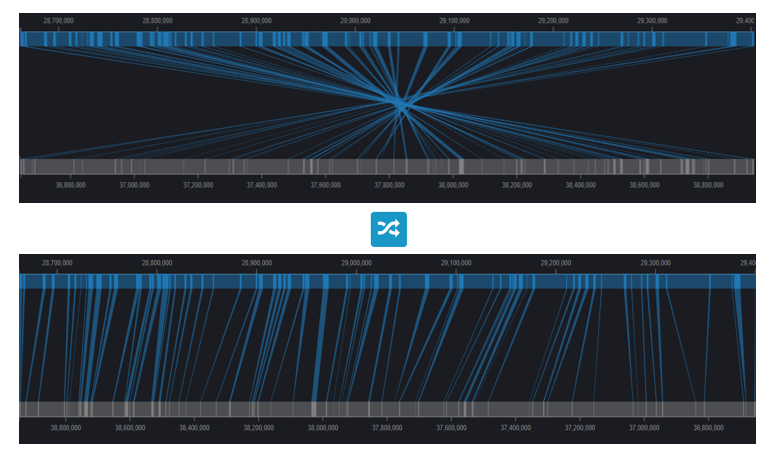
\includegraphics[width=1\linewidth]{images/ch_5_block_view_invert.PNG}
  \captionof{figure}{Conserved regions that have undergone reversals(top) can be flipped along the target genome using the toggle button to provide an uncluttered representation(bottom). } 
  \label{fig:ch_5_block_view_invert}
\end{figure} 

\subsection{Multi Genome Analysis Mode}
This mode of SynVisio is used to trace and analyze conserved regions between several genomes at once. It can be enabled through the configuration tab of SynVisio and offers 2 kinds of visualizations: Tree plot and Hive plot.

\begin{figure}
  \centering
  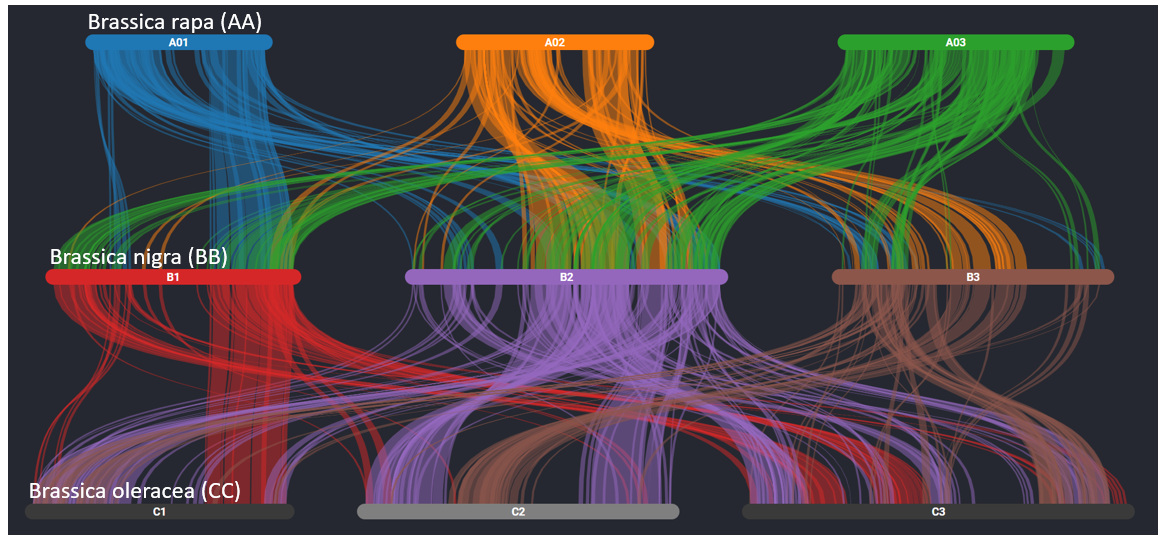
\includegraphics[width=1\linewidth]{images/ch_5_tree_plot.PNG}
  \captionof{figure}{Tree plot showing multi genome synteny between the three ancestral genomes from \textit{Brassica} genus.} 
  \label{fig:ch_5_tree_plot}
\end{figure} 

\textit{Tree Plot:} This view is an extension of the primary two-axis parallel plot that is used in the primary analysis mode (Figure \ref{fig:ch_4_dashboard}), but with additional rows that show pairwise synteny across multiple genomes. Users are first given the option to select the number of rows they need, and they then choose the chromosomes they need in each row individually. Chromosomes are stacked in multiple rows and conserved regions in the chromosomes in every row are linked bidirectionally (Figure \ref{fig:ch_5_tree_plot}). Starting from the top layer, every chromosome acts as a parent node and is linked to the chromosomes in the row directly below it if conservation exists, thus forming a tree-like pattern that can be used to look for conserved regions in ancestral species. Figure \ref{fig:ch_5_tree_plot} shows synteny between the first three chromosomes of three ancestral genomes of the \textit{Brassica} genus from the \textbf{Triangle of U} evolutionary model\cite{cheng2014genome}. Users are given the option to filter the conserved regions by clicking on a chromosome to visualize just the conserved blocks emerging from it at every layer. A dual filter toggle is also provided to ensure that chromosomal filtering occurs bidirectionally ( i.e., conserved links that both emerge from a chromosome into the the layer below and the conserved links that join into it from the layer above it are both filtered).

\begin{figure}
  \centering
  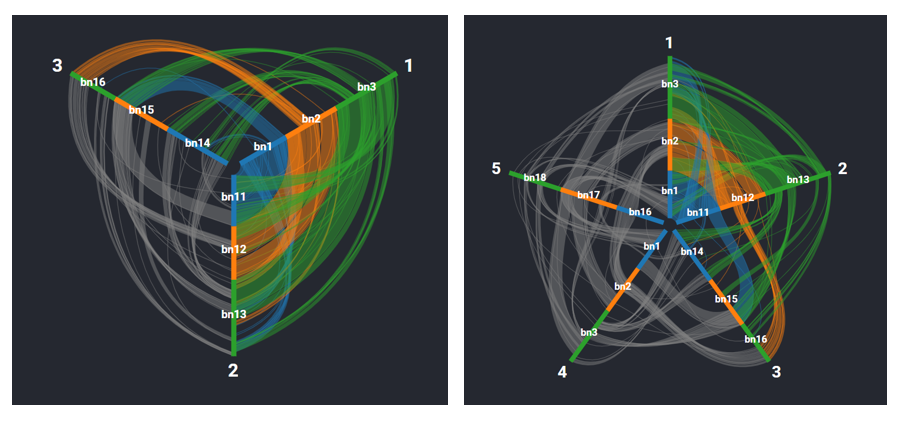
\includegraphics[width=1\linewidth]{images/ch_5_hive_plot.PNG}
  \captionof{figure}{Hive plots showing 3 way synteny(left) and 5 way synteny(right) in \textit{Brassica napus} respectively.} 
  \label{fig:ch_5_hive_plot}
\end{figure} 


\textit{Hive Plot:} These plots have recently been used in large scale network visualizations such as gene regulatory networks due to the high degree of perceptual uniformity that they offer\cite{krzywinski2011hive}. They have also been demonstrated as good alternatives for Circos \cite{krzywinski2009circos} style plots in representing three-way genome alignments. Hive plots are based on a linearized network layout where nodes are placed in radially-oriented axes, and edges are drawn between the nodes to encode additional information. In our tool, the nodes represent chromosomes, and they are ordered sequentially based on their order in the genome. The radial angles between the axes are chosen based on the number of selected axes. Conserved regions between the chromosomes are then linked through connecting ribbons which are drawn using Bezier curves with edge bundling to reduce visual clutter \cite{zhou2013edge}. Unlike the pairwise comparison scenarios, hive plots do not have a single source axis as all axes are uniform in a multi-way comparison scenario. Therefore, connected ribbons are not coloured to represent the chromosomes they emerge from and are instead left to be translucent gray. User interactions with the hive plot are used to select the source axis. When a user clicks on a particular radial axis, all the connected ribbons emerging from it are coloured based on the chromosomes they belong to in that axis. This form of variable encoding based on user choice can be useful in selectively identifying patterns for every genome represented in one radial axis. To use the hive plot, users first select the number of radial axes they need and then select the chromosomes to be encoded in each axis. The generated hive chart can then be annotated with chromosomal labels (hidden by default but can be toggled on/off using a checkbox present in the filter panel). The scales for the radial axes are calculated based on the genomic size of all the chromosomes included in the chart. This ensures that chromosomes that are small in terms of the number of base pairs, show up as smaller edges. This can further mean that the sizes of the radial axes of the hive chart can vary depending on the chromosomes that are represented in them. Our interface also provides a \textit{Normalized length} checkbox that can be toggled \textbf{ON} to make the hive chart axes equal in length increasing uniformity. This is achieved by using a variable linear scale for every axis while keeping its total length constant.

\section{Usability Features}
As SynVisio developed into a full-scale application, we were provided with several non-functional requirements from our research collaborators. For each of these requirements, we added features that do not change the existing visual encodings used in the system but rather enhance the overall user experience. 

\subsection{Track Annotation}
The ability to annotate visualizations with additional data in the form of tracks is a feature that is available in many genome browsers such as JBrowse, GBrowse, and UCSC Genome Browser\cite{skinner2009jbrowse,donlin2009using,karolchik2003ucsc}. However, it has not seen widespread adoption in the existing synteny analysis tools except for Mizbee,  AccuSyn, and GSV\cite{Meyer2009,accusyn,revanna2012web}. Showing annotation tracks can help researchers better understand the data under investigation because tracks such as gene counts and SNP (single nucleotide polymorphism) variations can highlight regions of interest in the entire genome. In our system users can upload a track along with their initial data file using a BedGraph file (a standard format used in representing continuous-valued data as tracks). Our system parses the data in the track file and automatically groups it based on the chromosomal widths into distinct regions for each chromosome so that the data can be loaded on demand when a user selects a particular set of chromosomes for their visualization. We also calculate the maximum and minimum values in the file and use them to generate a linear scale. We limit the number of tracks to prevent overcrowding in the visual representation.

\begin{figure}
  \centering
  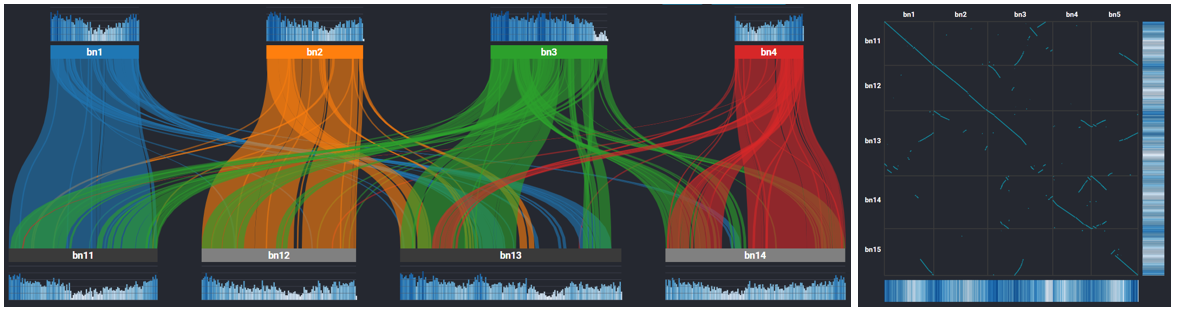
\includegraphics[width=1\linewidth]{images/ch_5_tracks.PNG}
  \captionof{figure}{Additional tracks showing gene count as a histogram in the Parallel plot (left) and as a heat-map in the Dot plot (right).}
  \label{fig:ch_5_tracks}
\end{figure}
When SynVisio detects additional track data in the system, it automatically provides a new button next to the chromosome selection panel called \textit{Toggle Tracks}, which controls the visibility of tracks in the visualization. We offer four types of tracks: heatmap, histogram, linechart and scatterplot. The heatmap uses a sequential colour scale to encode values in increasing order from white to dark blue. The same colour scale is also used for the histogram and the scatter plot as the default encoding scheme. The linechart alone does not use any colour encoding and is represented in a single base colour. All the graphical positions in the charts are rendered using the previously calculated linear scale which is also used to generate five equidistant grid lines for the tracks. For the parallel plot (Figure \ref{fig:ch_5_tracks} left), the tracks are added on the outer side of the visualization with one track sitting above the source genome and the other track sitting below the target genome. Since the tracks are accurately mapped to the chromosomes, the pill shaped design of the chromosome similar to karyograms (discussed in Section 2.2.2) is replaced with rectangles to ensure the start and the end of the chromosomes are consistent with the start and the end of the tracks. For the dot plot, the tracks are annotated along the \textit{x,y} axes on the opposite side of the chromosome labels (Figure \ref{fig:ch_5_tracks} right).


\subsection{Gene Search Panel}
SynVisio maintains an in-memory collection of all the genes present in the genome or multiple genomes under investigation in the interface. This can be used to quickly look up conserved regions that contain a particular gene of interest. This feature is presented in the \textit{Gene Search Panel} situated at the top of the dashboard (Figure \ref{fig:ch_5_gene_serach}). Users can type in a Gene ID and click on the search button. The system then checks the collection of genes and presents all matching alignments as clickable buttons along with information on the source and target chromosomes of the alignment and its orientation. Clicking on any alignment launches the chromosome mode of SynVisio between the pair of chromosomes that contain the alignment block, and the alignment block itself is highlighted in a pale white colour, as shown in Figure \ref{fig:ch_5_gene_serach}. 

\begin{figure}
  \centering
  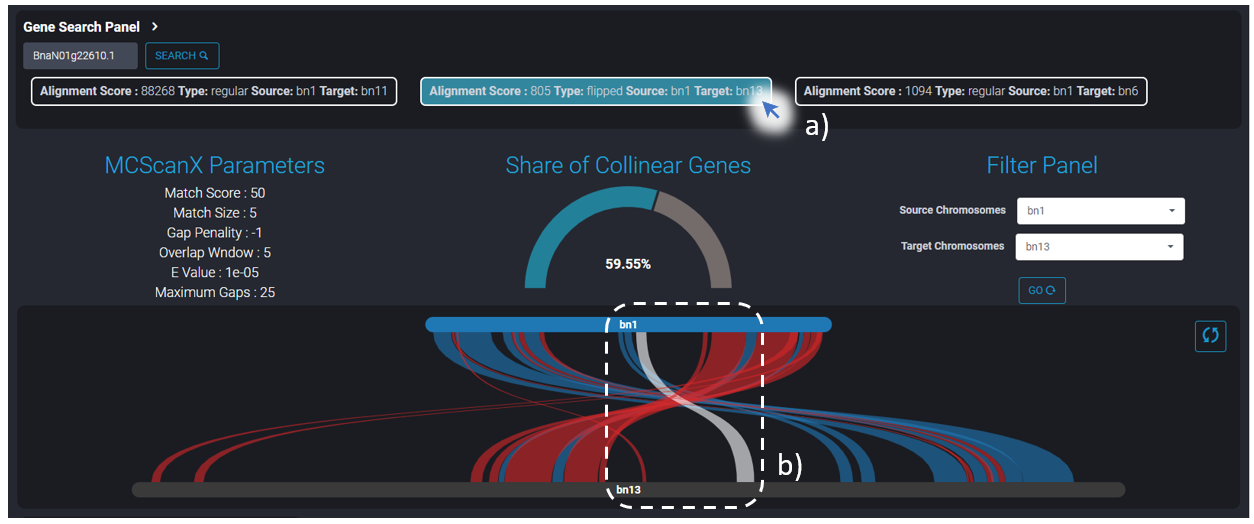
\includegraphics[width=1\linewidth]{images/ch_5_gene_serach.PNG}
  \captionof{figure}{Gene Search Panel in SynVisio, with matching alignments present as clickable buttons (a) that when clicked highlight the corresponding alignment (b).}
  \label{fig:ch_5_gene_serach}
\end{figure}


\subsection{Support to Map Unplaced Scaffolds}
Genome assembly is the process in which a genome is pieced together into a large number of contigs computationally from randomly sequenced reads (DNA/RNA segments)\cite{hunt2014comprehensive}. These contigs are then assembled into longer scaffolds which are in turn further assembled into chromosomes. However, due to lack of sufficient mapping information the position and orientation of certain scaffolds remains unknown and also many genome assemblies only assemble data to the scaffold level \cite{ensembl}. This makes it impossible visualize synteny as most synteny tools only offer mapping based on chromosomal order. SynVisio attempts to solve this problem by letting users visualize the synteny between unplaced or unlocalised scaffolds. By default SynVisio ignores Scaffolds regions as there can be quite a lot of them cluttering the visualization, however users can opt out of ignoring scaffolds. This will give users a list of scaffolds to select in the source and target chromosome list in the filter panel at the top of the dashboard. This feature is particularly important to users who would like to visualize collinearity between unplaced scaffolds and known sequenced genomes to improve their genome assembly results. 


\subsection{Image Export}
Most synteny browsers such as MultiSyn, Synteny Portal, and GSV\cite{baek2016multisyn,lee2016syntenyportal,revanna2011gsv} have the option to export images; an exception is Mizbee\cite{Meyer2009} which is designed more for analysis than image generation. SynVisio can work both as an analysis tool and can also generate high-quality publication ready images when required. SynVisio renders visualizations on screen as SVGs( a transform and scale-invariant vector graphics format), and these can be downloaded using the \textit{export toggle} provided as a floating button situated in the bottom corner of the screen. Furthermore, SynVisio exports visualizations based on the current settings of the system as users interact with it in real-time (changes such as adding tracks, filtering out low similarity score blocks and highlighting a particular chromosome are all retained in the exported image). A final advantage of exporting images in SVG format is that these images can be edited and the colours of the individual elements changed using vector graphic editors like Inkscape and Adobe Illustrator.

\subsection{Revisitation Support}
Multi-scale visualization systems are effective at exploring large datasets because they help researchers follow the visual information seeking mantra of \textit{overview first, zoom and filter}, followed by \textit{details on demand}\cite{Shneiderman96theeyes}. They achieve this by changing the visual representation of the data at different levels of abstraction as the user zooms in for closer inspection\cite{Stolte}. This process however, can cause the user to lose an overall context of their position in the visual space as they constantly need to switch between different kinds of visual representations.
Although humans are good at leveraging spatial cognition to remember locations of objects in information workspace tasks\cite{datamountain}, context switching can disrupt this ability. To assist the user in navigating to previous states of the system, SynVisio lets users keep track of their actions through a visual snapshot feature. It preserves the sequence of actions that led to the current state of the visual interface in a snapshot. Users can store this snapshot by clicking on the floating camera button at the bottom left corner of the interface. Snapshots are stored sequentially and are available for revisitation at the \textit{Snapshot Store Panel}. Clicking on any snapshot in the panel automatically recreates the stored visual state of the system. The snapshots, however, are stored only as an in-memory collection in the system and so do not persist over page reloads or when users switch the input data files.


\section{System Architecture}

Recent trends in software development have shown an increase in the development of internet-based web applications that are built using HTML5, JavaScript and CSS3. This is due to the availability of web applications and their device-agnostic design that ensures that they run independently of operating system or device type. Although some synteny browsers have been developed as native applications (Mizbee and SyMAP\cite{Meyer2009,soderlund2011symap}), most recent synteny browsers like MultiSyn, mGSV and Synteny Portal\cite{baek2016multisyn,revanna2011gsv,lee2016syntenyportal} all adopt a web-based approach. Following this trend, we developed SynVisio as a web-based application that can be accessed for free through the internet at \url{https://synvisio.usask.ca}.

A choice must be made between two main design patterns for web applications: single-page or multi-page application. The choice is based on the content being served. Single-page applications request content markup and data independently and render pages dynamically in the browser through JavaScript. This makes them fast and responsive despite the initial delay in loading all content in a single bundle during page load. There are no subsequent page reloads and all further requests are purely for data which has a significantly smaller payload. Multi-page applications, on the other hand, follow a more traditional approach with changes and interactions being sent to the server, which responds back with a new page to be rendered by the browser. This additional communication between the browser and the server can make these systems cumbersome to use due to added delay. However multi-page applications are more secure compared to single-page applications which can be susceptible to cross-site scripting (XSS) attacks.
Although users aren't concerned with software architecture, as they focus on tasks and not the structure of a system, it can be a determinant for the usability of any system. Proper information architecture should offer users logical structures that can aid them in navigating towards the right answers and completing their tasks\cite{rosenfeld2002information}. Thus for SynVisio, we adopt the single-page architecture design and render visualizations in the browser instead of having them shipped from a remote server, as this allows for users to interact with them in real-time and offers a smooth interactive experience\cite{nielsen2010visualizing}. 

This architecture model where data processing is managed locally in the client machine is called a thick client model. It ensures that all the data files that researchers upload to our website remain secure within the same browser instance and are not sent to any other remote server. However, processing data files in the web browser comes with its own set of complications as JavaScript has a single threaded environment and any intensive data processing can block the main thread limiting user interactivity in the page. To address this issue we use the web workers API to spawn background scripts that can handle computationally intensive tasks without blocking the main user interface\cite{webworkers}. Every user-uploaded file is processed in an independent thread through a web worker and the processed results are then combined to form an in-memory dictionary of all the genomic links, classified based on the chromosomes present in the genome. This dictionary is then used whenever a user selects a pair of chromosomes to query the required set of genomic links for visualization.

The web interface of SynVisio is built using two JavaScript libraries: React.JS\cite{react} to handle user interactions and render content, and D3.JS\cite{d3js} to generate visualizations.
React is a popular JavaScript library maintained by Facebook\cite{facebook} that is used in building user interfaces in single-page applications. It can efficiently manipulate the representation of a webpage which is called the document object model (DOM). It does this through a process of reconciliation with an in-memory representation of the actual DOM called the virtual DOM. This is particularly useful in our scenario as all visualizations are rendered through vector graphics and so are part of the actual DOM structure.Thus as the size of the data being visualized increases there is a corresponding increase in the number of visual elements in the DOM. However by using React we can handle large DOM networks efficiently by deferring updates only when necessary. The second major advantage to using React is that it follows a component-based model where every part of the interface is built using a set of reusable components that render differently based on the data being passed to them. This enables us to rapidly switch the generated visualizations on the screen by simply modifying the underlying data provided to the component. This is particularly useful in implementing interactive real-time filtering as any filtering done to the underlying dataset is reflected onto the actual visualization. This feature is also used in providing support for the revisitation feature discussed in section 5.3.4. Every saved snapshot is essentially a data object that is stored and passed to the graphical component to recreate the required visualization.

All visualizations in SynVisio are rendered as scalable vector graphics(SVG) with the coordinate values of the underlying graphical elements being calculated using D3.JS. These include the mathematical calculation involved in the interpolation of points that connect conserved regions and scale transformations from genomic distances to pixels. Finally, SynVisio can switch to rendering using the HTML Canvas (an immediate-mode pixel-based drawing surface) instead of vector graphics when there are more than 20,000 graphical elements in a visualization, as SVG performs poorly at these scales. This also limits the user interactions that are possible with the visualization (as detecting mouse interactions can be slow), and a warning message is shown to the user to select a smaller subset of the dataset or an alternate representation with fewer visual elements. This adaptive mode of SynVisio was built to ensure that even extremely large datasets can be viewed in the system without a reduction in performance.


\chapter{Evaluation}

SynVisio was made publicly available to use for free on the internet on September 2018. A stable version was deployed in the start of 2019 and ever since then, it has been used by several researchers across the world in exploring genomic conservation in a wide variety of organisms. To evaluate our system we conducted semi-structured interviews with 5 domain experts from the three research groups we were collaborating with and one of the expert was a bioinformatician who worked across all three research groups. The interviews were conducted either through phone or an in person meeting and lasted around 45-60 minutes. Researchers were first asked about the relevance of synteny visualizations in their field of research and then asked to give their opinion on the different features that SynVisio offers and how they helped in exploring synteny in their particular dataset. We summarize their feedback on the system through three case studies, one from each research collaborator group, presented in the sections below. To provide evidence on the effectiveness of our system \textit{in the wild} we explored user activity logs on the website for a period of 12 months through google analytics. Finally to demonstrate the open-ended design of SynVisio we provide examples of genome databases for silk worm and two other species that were extended to show synteny visualizations using the open sourced code of SynVisio.

\section{Case Studies}

\subsection{Wheat\textit{(Triticum aestivum)}}
What is one of the most widely cultivated crops in the world and plays an important role in human nutrition. Being a common cereal wheat genomes are highly diverse and spread over a large geographical range. The genome is capable of tolerating mutations and extensive hybridization to a great level which is why it has been able to adapt to such a wide variety of environmental conditions\cite{wheatinfo,10wheat}. Wheat is also one of the \textit{neolithic founder crops} that were the first to be domesticated almost 10000 years ago.
Bread wheat(AABBDD) is a hexaploid genome and is the result of series of hybridization events between three ancestral genomes A Donor(Triticum urartu), B Donor(Aegilops speltoides) and D Donor(Aegilops tauschii) which makes it an interesting subject for synteny analysis. Our collaborators were part of a research team involved in sequencing a high quality version of the wheat genome. Since the wheat genome is extremely large and complex synteny analysis can help researchers in assessing the quality and contiguity of the genome assembly though alignments between the sub genomes (A,B and D).

Our collaborators relied on visualizations generated by SynVisio to present and summarize their sequence assembly results - \textit{``the images have been used in presentations, academic meetings such as the international wheat congress and also at the plant-animal genome conference.'' (R1)}. While they used Circos style plots for research publications earlier, they mentioned that the multi level representations in SynVisio were far more useful for genomes like wheat with many chromosomes in it - \textit{``This tool is better than a Circos plot, especially when comparing multiple genomes, circos can be limited because you are seeing too many chromosomes in one circle and so are losing information ... a stacked layout like yours is easier to see.'' (R4)}. One collaborator in particular also appreciated the system for its ability to handle large datasets like wheat - \textit{``this is really neat. this is also very useful...a single wheat chromosome is vast and wheat has 21 of those placing stress on an analysis pipeline in terms of computational complexity...it is also very repetitive...'' (R1)}.
Feedback provided by this research team was also used in adding support for hive plots which offer a very intuitive representation to compare multiple sub genomes in crops like wheat as shown in figure \ref{fig:ch_6_wheat}. Our collaborators in this team plan on publishing images generated using SynVisio and have already used it to create a portal for researchers to compare 12 different wheat cultivars for the 10+ Wheat Genomes Project. Users can use this portal to select any two varieties from 12 different wheat cultivars and then compare genomic conservation between them using SynVisio\cite{10wheat,wheatinfogithub}.

\begin{figure}
  \centering
  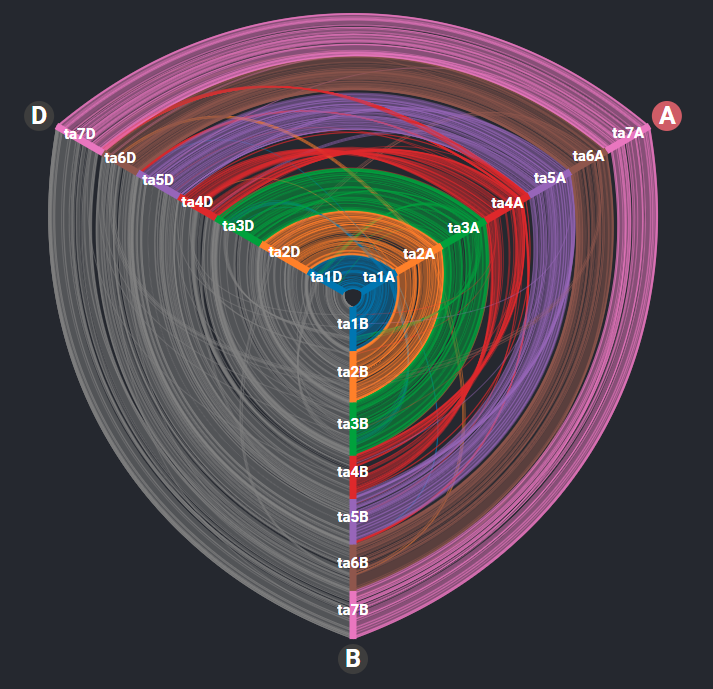
\includegraphics[width=0.72\linewidth]{images/ch_6_wheat.PNG}
  \captionof{figure}{Genomic conservation between the three sub genomes A,B and D of Wheat(Chinese Spring Variety) shown through a Hive plot in SynVisio.}
  \label{fig:ch_6_wheat}
\end{figure}


\begin{figure}
  \centering
  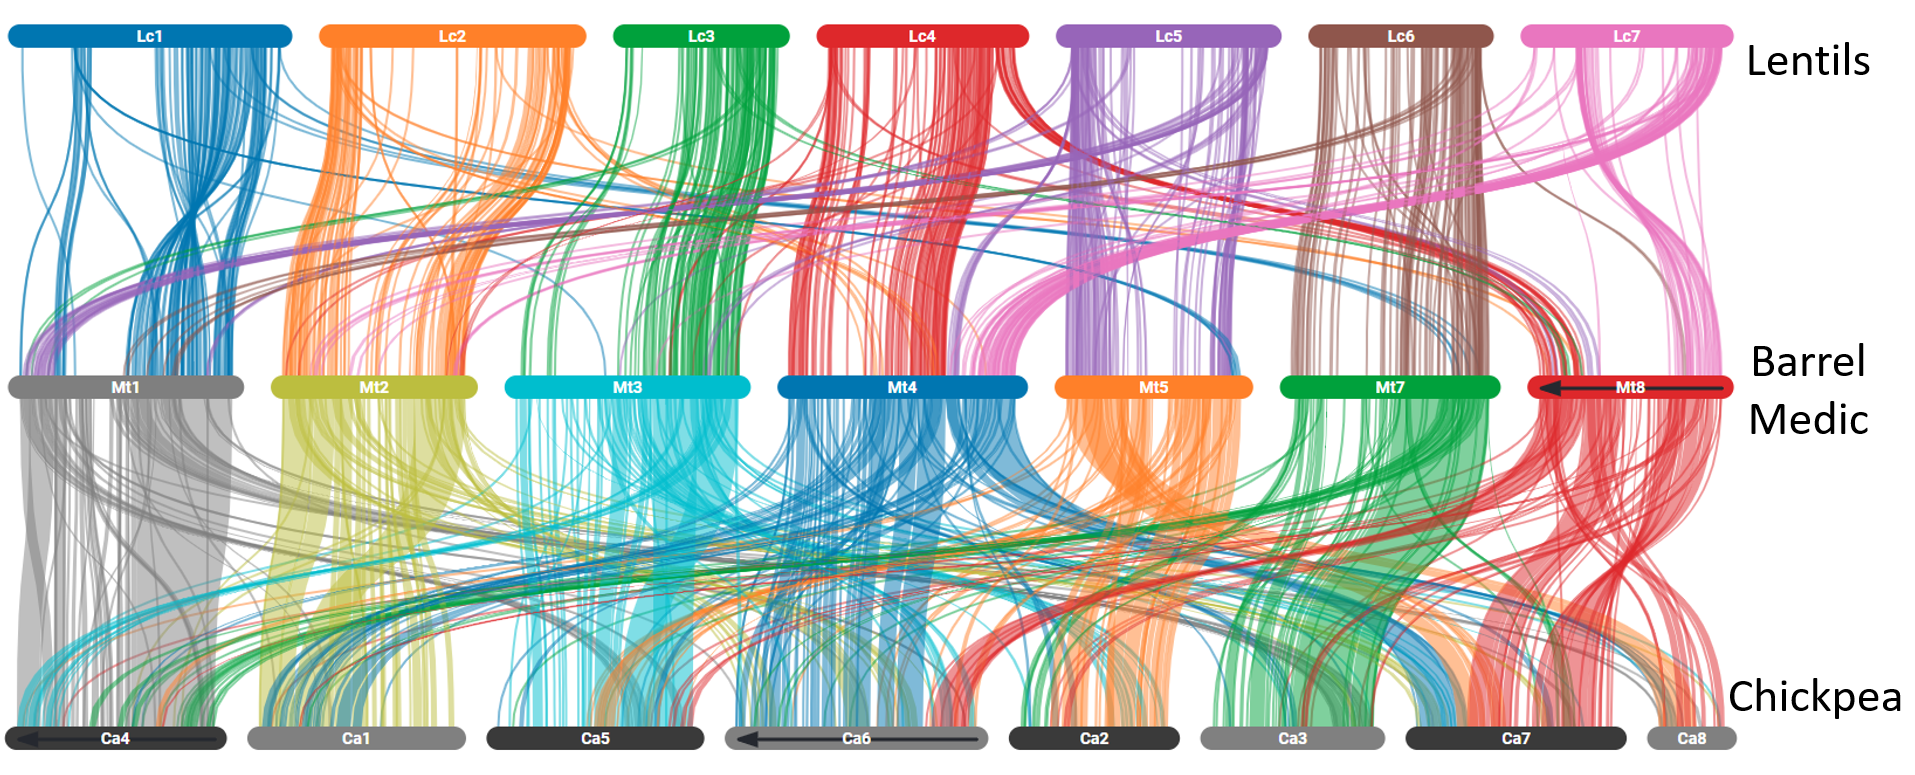
\includegraphics[width=1\linewidth]{images/ch_6_lentils.png}
  \captionof{figure}{Collinearity between Lentils(Lc), Barrel Medic(Mt) and Chickpea(Ca) presented through a Tree view plot. The ordering(Ca) and orientation(Mt8,Ca4 and Ca6 - flipped) of some chromosomes have been changed to reduce visual clutter.}
  \label{fig:ch_6_lentils}
\end{figure}


\subsection{Lentils\textit{(Lens culinaris)}}
Lentil is an important legume crop that is grown globally as a valuable source for dietary protein. It also plays a crucial role in food security in developing countries along with other legume crops like Chickpea(Cicer arietinum)\cite{varshney2013draft}. Lentils can be made more resistant to diseases and weed infestations by increasing the genetic diversity of the genome through hybridization between disease resistant wild varieties. This however requires mapping the traits through molecular markers to assess their diversity. Our collaborators relied on comparative genomic mapping to leverage information from a model legume species like Barrel Medic(Medicago truncatula) onto less studied crop species like lentils and chickpea due to lack of common markers.

Unlike the wheat genome, synteny analysis requirements for this project were centered around cross synteny between species rather than self synteny. Due to the large size difference in the genomes between Lentils(4Gbp) and Chickpea(~740Mbp) the first version of SynVisio was not able to generate legible charts as the Lentil chromosomes were extremely wide compared to chromosomes from the other species and so a special feature was added to have variable scales at different levels. Our collaborators were pleased with the updated view and also remarked on the multiple visual representations provided in the genome view - \textit{``I think it's quite good, I do really like that there's also the dot plot, in the corner, so that if anything is a little bit unclear, from the parallel view, you can kind of refer back to that.
'' (R5)}. Because this was a cross synteny analysis between several genomes, researchers mentioned that the Tree view was particularly helpful in summarising large scale chromosomal rearrangements and inversions while still keeping the different genomes visually distinct as shown in figure \ref{fig:ch_6_lentils}. They also compared it to circos plots and remarked on its usability - \textit{``It's like the circos plots are beautiful but you can't do anything with it. Whereas this, the tree-view in particular, is very aesthetically pleasing and that's the kind of thing that you can show to your collaborators and you can also understand it, at the same time, and then the interactive nature of it helps too...
(R5)''}. Reseachers froom this group have also used SynVisio to study genomic conservation in other legumes like the Tepary Bean (Phaseolus acutifolius) and are planing on using it to generate images for their research publications in future.

\subsection{Canola (Brassica napus)}
Canola is an important oil seed crop in the world as it is an excellent source for both animal feed and high quality edible oil\cite{shahidi1990canola}.It is an allotetraploid (4 copies - AACC) species that was formed through interspecific hybridization between diploid ancestors Brassica rapa (A Donor) and Brassica oleracea (C Donor)\cite{parkin1995identification}. Studying this genomic conservation can help researchers in looking at genetic variations that are advantageous from an evolutionary perspective in polyploids like Canola. Our collaborators from this research group were particularly interested in using comparative mapping to understand the level of genome duplication in modern brassica cultivars and the occurrence of genomic rearrangement in the evolution of these varieties from a common ancestor. This meant that they needed to visualize both self synteny between Canola itself and also cross synteny between canola and its closely related species. - \textit{``...in polyploid plants where there are many genomic rearrangements, visualization is really useful because there is lots of information and its really complicated for us to understand without an overview... (R2)''}

SynVisio also helped researchers in this team at refining their assemblies - \textit{``Our assembly got better when we upgraded our sequencing from short read to long read sequencing technology as more regions are assembled. This tools helps us visualize that improvement ...(R2)''}. Regarding the visual representations one collaborator remarked that the parallel plot representation was better at showing genomic conservation than dot plots - \textit{``We have always used dot plots but these (parallel plots) are visually more intuitive...when chromosomes start breaking apart its much more difficult to follow where things are going in that big square and in this its easier to play around...Its much easier to trace things and work out where you are...(R3)''}. Researchers from this team have used visualizations generated by SynVisio at several conferences such as PAG (Plant Animal Genome) 2019 \cite{brassicapag} and also in a recent publication describing long read assemblies of two diploid Brassica species\cite{perumal2020high}.
 
\section{Usage analysis based on Google Analytics Logs}
Methods – How we instrumented the program to gather the data.
Decide on a set of interview questions 
Come up with the interview format – Where they use the tool and then they describe the tool
Which views do they most often.
What are the advantages and we an ask them the question does this solve the problem of interactivity – WE ask them how they did it before and if this tool solves it ?
Compare no of steps used to create a chart before and after synvisio.

\section{Interpretations and Findings}  
Summarize what worked well and what didn’t work well .
Which sections where used frequently and why 
How are we doing on these initial problems – What we set to do and how has our system performed.
For example Availability – Just show the internet logs


\chapter{Discussion}

In this chapter, we discuss the the insights gained from building each of the unique features of our system and the design choices that went into their development. We also look at how some of these features can be extended to support additional genomic analysis tasks. We then explore some of the limitations of our current system based on the feedback gathered from our user evaluation study and possible improvements that can be made in the future.

 \section{Design Implications}
 
\begin{itemize}
    \item \textbf{Input Files and Formats} - Genomic conservation can be detected through a wide range of tools, which means that it can be represented in a wide variety of file formats depending on the type and the level of information about conservation of gene order.
    Although some tools like Mizbee have relied on users to supply input in a standardized format, this is not a viable solution as this often means users will have to rely on a custom script to transform their analysis files into the required format. Visualization tools like SynVisio and Mizbee are part of a larger ecosystem of genomic analysis tools. So they need to offer at least partial connectivity between such tools which means outputs of most analysis systems should be directly supported in visualizations tools without the need for intermediate processing. In an effort to address this developers should consider building systems that offer support for heterogeneous data. For example, SynVisio currently supports inputs from several popular tools such as collinearity files generated by MCScanX or Orthologous files generated by Dagchainer with also partial support for MUMmer output files. 
 
    \item \textbf{Web Accessibility} - Most existing genomic visualization tools are desktop applications or packages in languages such as R, Python, or Perl, however, there has been a gradual shift towards the web in the recent years. Although desktop applications are efficient at utilizing system resources, they are limited in their accessibility as they are not often supported in all operating systems and require extensive customization from developers as they are platform dependant. Web applications, on the other hand, are platform independent and can be built once and used everywhere thus requiring less development effort. Even though web apps are limited in their processing capability, they can rely on remote servers for intensive processing, and some applications like SynVisio also rely on web workers to process data in parallel threads for more efficient data processing. This easy accessibility and low-cost maintenance of web apps coupled with support for collaborative work mean that web applications should be the first choice for developers of visualization tools in the future.
    
    \item \textbf{Multi Layout and Multi Scale Views} - 
    Genomic data can be analyzed at multiple resolutions and the visual representations vary at each level. At the genome level, visual representations are chosen to emphasize approximate positions of the conserved regions and their chromosomal identifiers. This can be useful in scenarios such as during genome assemblies when errors or breaks in chromosomes can be easily identified. However, when looking at the chromosome level, orientation of the conserved region is also highlighted and finally at the individual gene level emphasis is placed exclusively on the order of collinear genes and their exact function and location in the genome. Visual representations can also vary based on the task at hand. For example, dot plots are a popular choice for summarizing large scale datasets as they offer a compact representation of both the position and orientation of conserved regions. However, their orthogonal representation is difficult to understand, making them an unpopular choice for browsing and locating selective conserved regions in comparison to parallel plots. Other such examples are stacked parallel plots which are good at tracing collinear regions across several genomes. Thus in designing genomic visualization systems, developers should rely on a combination of visual representations or provide users the choice to switch between different representations based on the task at hand. 

    \item \textbf{Visual Navigation and Linked Views} - When exploring genomic data, visualization systems can provide users several ways to traverse the different representations at each genomic scale. However, the most intuitive way to explore such a dataset would be to start at the genome level and drill down all the way into the individual gene level. So visualizations at each level should be provided with interaction techniques to filter and zoom into a particular part of the dataset which can then be viewed in a different visualization at the next inner level. This form of tiered navigation combined with the support for revisitation at any point can help researchers in easily going back and forth between the levels and exploring a large number of scenarios without losing context. Also, a major part of analyzing genomic conservation involves comparison, and providing linked multi-views that are different representations of the same information can help users in contextualizing the conservation and better understanding it.
    
    \item \textbf{Linear vs Non Linear Representations} - Genomic data is usually linear and so the best form of representing such data would be a linear representation such as a dot plot or a parallel plot but circos style plots which are a form of non-linear representation are still quite popular in genomic visualizations as they are aesthetically pleasing and offer a compact picture. However, based on observations from our user evaluation, several users found circos plots challenging to navigate for an in-depth analysis. This is primarily due to the non linear curves in these plots than can make it difficult to identify connections between distinct groups which in this case are chromosomes ordered in a circular layout. While linear representations like parallel plots can be stacked on top of each other to represent conservation between multiple genomes, circular layouts can only handle a limited number of chromosomes in the central layer before they become difficult to comprehend due to close proximity between the chromosomes. Part of the compact nature of the circos style plot arises from its ability to stack several circular layers on top of each other to represent several tracks, however, the radial nature of this design means that tracks in the outer layers are always larger than the tracks in the inner layer. This can lead to visual bias where patterns in the outer layers are more prominent than patterns in the inner layers.
    
    \item \textbf{Adaptable Genome Scales} - Genomic data can be incredibly diverse in size and so systems visualizing such information need to automatically adapt to different scales of data instead of relying on a standard scale. Some plant genomes like wheat are extremely large (17 Gigabases) and quite dispersed due to which the genes are quite small and so when visualizing this information, SynVisio provides users 2 additional levels to magnify the dataset. Similarly, when visualizing extremely small genomes such as viral genomes (30 Kilobases) the system automatically loads up the data in the smallest possible resolution directly at the gene level as shown in Figure \ref{fig:ch_7_viral} which compares similarity between two coronavirus strains that led to global pandemics. This disparity in genome sizes can also be an issue when comparing multiple genomes with a vast difference in their sizes. In such scenarios, the visualization system should provide users an option to have different scales for each of the genomes instead of relying on a single normalized scale among the genomes. 
\end{itemize}

\begin{figure}[h]
  \centering
  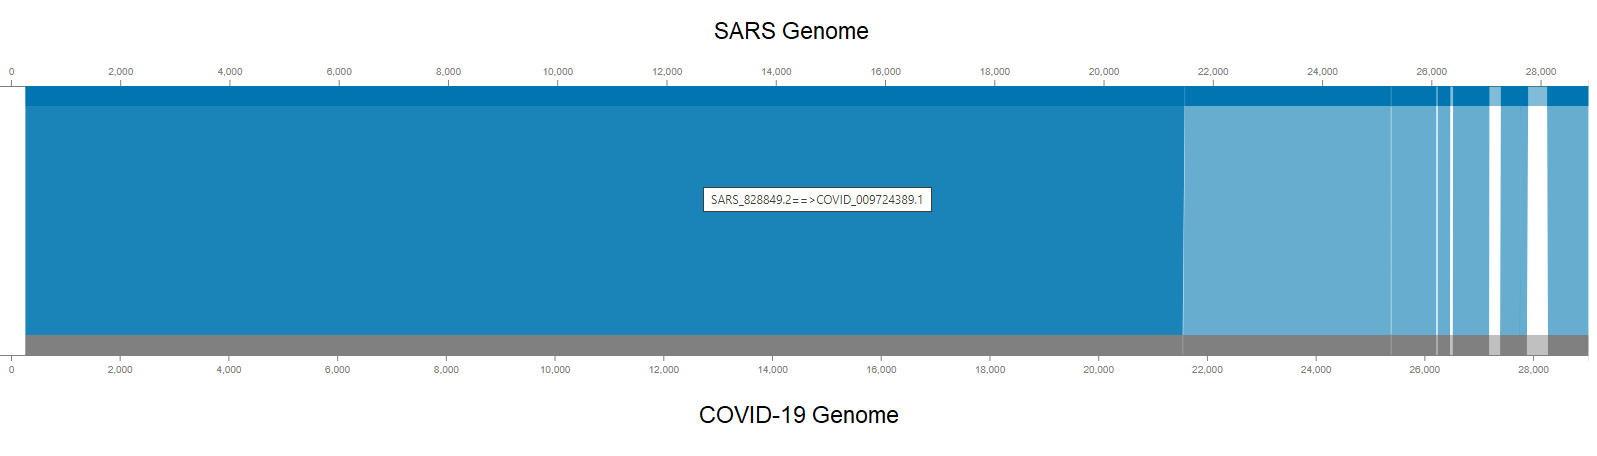
\includegraphics[width=1\linewidth]{images/ch_7_viral.PNG}
  \captionof{figure}{Extensive similarity between genomes of the SARS Virus (2003 pandemic) and the COVID-19 Virus (2019-2020 pandemic) with the RNA responsible for a single protein highlighted in a darker shade.}
  \label{fig:ch_7_viral}
\end{figure}


 \section{Limitations and Future Work}
 
 Although SynVisio was designed to handle a wide variety of scenarios, there are still certain issues with our system that can be improved through additional changes in the future. 
 
 \begin{itemize}
    \item The first and major limitation of our system lies in the dependence on an external tool (MCScanX, DAGChainer or Mummer) to detect conserved regions. This was mentioned as a bottleneck by several of our users in analyzing their datasets. But the complexity involved in detecting similarity between two given sequences and running a collinearity detection software cannot be achieved through the existing web system as it is computation intensive. A possible way in which this can be solved in the future is by setting up a dedicated remote server that can accept sequences uploaded by users to perform synteny detection on the cloud and then send the results back to the web system to be visualized. This would also give users greater flexibility in changing the different parameters involved in detecting conserved regions such as the E-value  to look at more distant matches.    
    
    \item SynVisio is currently opinionated in determining the visual scale of the genome. Genome scales are calculated based on the available screen width and the size of the genome in base pairs and every chromosome is normalized accordingly. But users are given the option to override the normalization and have independent scales for each genome when comparing multiple genomes. This can lead to confusion when two genomes are stacked parallel to each other, and both stretch to fill the available width causing users to lose context of the size of the genomes. To address this confusion in future, we can provide information in the form of tracks or scales indicating the size of the genome in Kilo-bases or Mega-bases.
    
    \item SynVisio automatically sorts chromosomes alphanumerically in each genome to determine their layout. These chromosomes are then presented from left to right and oriented in the same direction. However, in some cases, this layout can cause the ribbons connecting conserved regions to excessively cross each other, making it difficult to understand the relation between the two genomes. In such scenarios, it would be helpful if users are provided an option to declutter the layout by reordering the chromosomes or reversing the orientation of each chromosome. This can be achieved in the future by developing a dedicated layout editor that lets users manual drag chromosomes around and reverse them if needed to create a more organized layout.
    
    \item Visualizing syteny in stacked parallel plots is an excellent way to trace conserved regions across multiple genomes. However, researchers are often also interested in understanding the evolutionary relationship between a given set of genomes along with an overview of the conserved regions between them. Evolutionary relationships among genomes are commonly represented as phylogenetic trees evolving from shared ancestors. Combining such a representation along with the existing parallel plots between genomes would be a significant improvement to SynVisio and offer researchers an easy way to analyze novel datasets such as the pan-genomes of different species.
    
    \item Although SynVisio lets users explore genomic data from the genome level all the way down to the individual genome level, it cannot show the actual nucleotide or the protein sequence alignment within every gene. This limitation arises due to the large size of FASTA files which cannot be loaded directly onto the Web interface. However, presenting this information can help researchers in understanding the extent of similarity in the gene alignment and gain additional information about the function of the gene and the protein it codes for. For most annotated genes, several online databases exist that curate this information and present it in a easily accessible manner such as genomeDB and NCBI. In future, we would like to link every gene in the gene level directly to their entries in preexisting databases, such that clicking on any gene would automatically open up the FASTA entry along with information about that gene in a new tab of the browser.    


\end{itemize}
 

\chapter{Conclusion}

Comparative genomic research plays a vital role in studying genome evolution and ancestral genome reconstruction. However, despite the availability of high-resolution genomic data, research in this field is being throttled due to the lack of proper analysis tools. While some analysis tasks can be automated to deal with the high volume of data, other tasks still require manual interpretation such as synteny analysis. Visualizing data in such scenarios can help researchers in their analysis by offloading part of the cognitive load required in processing information onto humans' inherent capacity for visual perception. Visualizing synteny blocks can aid researchers in understanding the location size and orientation of conserved genomic regions. Although some tools do exist for synteny analysis, they are limited in their usability and offer very little interactivity needed to explore complex datasets. Our primary contribution in this research work is SynVisio a synteny analysis tool that offers genomic researchers different ways to visualize and explore genomic data. Researchers can access the tool through a public web-based interface and directly upload their synteny analysis files. Information can be analyzed in a single level analysis mode through pairwise comparative visualizations such as linear parallel plots and dot plots. Alternatively, researchers also have access to a multi level analysis mode where syntenic blocks can be visualized through hive plots or stacked parallel plots to trace genomic conservation over multiple levels or between several genomes at once.

Our second contribution was in adding interactive support to our system to help researchers in refining and enhancing their datasets. All visualizations are accompanied by a filter panel to modify the generated visualizations in real-time. Syntenic blocks can be filtered based on the level of similarity (score or number of genes in a block) or the probability of the match (E value) depending on the underlying genomic question. Researchers can also augment certain visualizations such as parallel plots and dot plots with tracks representing additional information such as gene density or count of SNPs. These tracks are in the form of heat-maps, line charts, scatter plots or histograms. The tracks along with all visualizations can also be exported in publication-ready formats.

Our third contribution is providing support for revisitation. Synteny analysis is an exploratory task that requires researchers to investigate conservation at multiple genomic resolutions. Such exploratory analysis requires users to switch between multiple visualizations under different filter parameters. This switching can, however, cause them to lose context of their position in the dataset. SynVisio avoids this by providing users the option to snapshot the state of the system at any point in their exploratory analysis for easy and quick revisitation. This along with other features such as searching for genes in syntenic blocks, can be useful to researchers, particularly in exploring large datasets.

SynVisio has been developed as a modular component that can be reused in existing online genomic analysis tools, and the source code for the system has been open-sourced to facilitate the rapid dissemination of our work into other scenarios. Several researchers are currently using our system across the world either directly via the web interface or through the integration of our system into their existing tools. We also plan on adding additional features to the system in the coming year to offer support for other kinds of genomic analysis tasks.


%%%%%%%%%%%%%%%%%%%%%%%%%%%%%%%%%%%%%%%%%%%%%%%%%%%%%%%%%%%%%%%
% SUBSEQUENT CHAPTERS (or \input's)  GO HERE
%%%%%%%%%%%%%%%%%%%%%%%%%%%%%%%%%%%%%%%%%%%%%%%%%%%%%%%%%%%%%%%

%%%%%%%%%%%%%%%%%%%%%%%%%%%%%%%%%%%%%%%%%%%%%%%%%%%%%%%%%%%%%%%%
% The Bibliograpy should go here. BEFORE appendices!
%%%%%%%%%%%%%%%%%%%%%%%%%%%%%%%%%%%%%%%%%%%%%%%%%%%%%%%%%%%%%%%%


% Typeset the Bibliography.  The bibliography style used is "plain".
% Optionally, you can specify the bibliography style to use:
% \uofsbibliography[stylename]{yourbibfile}
\uofsbibliography{reference.bib}

% If you are not using bibtex, comment the line above and uncomment
% the line below.  
%Follow the line below with a thebibliography environmentand bibitems.  
% Note: use of bibtex is usually the preferred method.

%\uofsbibliographynobibtex


%%%%%%%%%%%%%%%%%%%%%%%%%%%%%%%%%%%%%%%%%%%%%%%%%%%%%%%%%%%%%%%%%%%%%%%%%
% APPENDICES
%
% Any chapters appearing after the \appendix command get numbered with
% capital letters starting with appendix 'A'.
% New chapters from here on will be called 'Appendix A', 'Appendix B'
% as opposed to 'Chapter 1', 'Chapter 2', etc.
%%%%%%%%%%%%%%%%%%%%%%%%%%%%%%%%%%%%%%%%%%%%%%%%%%%%%%%%%%%%%%%%%%%%%%%%%%

% Activate thesis appendix mode.
\uofsappendix

% Put appendix chapters in the appendices environment so that they appear correcty
% in the table of contents.  You can use \input's here as well.
\begin{appendices}

\chapter{Sample Appendix}

Stuff for this appendix goes here.

\end{appendices}

\end{document}
